\documentclass[a4paper,12pt,twoside]{memoir}

% Castellano
\usepackage[spanish,es-tabla]{babel}
\selectlanguage{spanish}
\usepackage[utf8]{inputenc}
\usepackage[T1]{fontenc}
\usepackage{lmodern} % Scalable font
\usepackage{microtype}
\usepackage{placeins}

\RequirePackage{booktabs}
\RequirePackage[table]{xcolor}
\RequirePackage{xtab}
\RequirePackage{multirow}

% Links
\PassOptionsToPackage{hyphens}{url}\usepackage[colorlinks]{hyperref}
\hypersetup{
	allcolors = {red}
}

% Ecuaciones
\usepackage{amsmath}

% Rutas de fichero / paquete
\newcommand{\ruta}[1]{{\sffamily #1}}

% Párrafos
\nonzeroparskip

% Huérfanas y viudas
\widowpenalty100000
\clubpenalty100000

% Imágenes

% Comando para insertar una imagen en un lugar concreto.
% Los parámetros son:
% 1 --> Ruta absoluta/relativa de la figura
% 2 --> Texto a pie de figura
% 3 --> Tamaño en tanto por uno relativo al ancho de página
\usepackage{graphicx}
\newcommand{\imagen}[3]{
	\begin{figure}[!h]
		\centering
		\includegraphics[width=#3\textwidth]{#1}
		\caption{#2}\label{fig:#1}
	\end{figure}
	\FloatBarrier
}

% Comando para insertar una imagen sin posición.
% Los parámetros son:
% 1 --> Ruta absoluta/relativa de la figura
% 2 --> Texto a pie de figura
% 3 --> Tamaño en tanto por uno relativo al ancho de página
\newcommand{\imagenflotante}[3]{
	\begin{figure}
		\centering
		\includegraphics[width=#3\textwidth]{#1}
		\caption{#2}\label{fig:#1}
	\end{figure}
}

% El comando \figura nos permite insertar figuras comodamente, y utilizando
% siempre el mismo formato. Los parametros son:
% 1 --> Porcentaje del ancho de página que ocupará la figura (de 0 a 1)
% 2 --> Fichero de la imagen
% 3 --> Texto a pie de imagen
% 4 --> Etiqueta (label) para referencias
% 5 --> Opciones que queramos pasarle al \includegraphics
% 6 --> Opciones de posicionamiento a pasarle a \begin{figure}
\newcommand{\figuraConPosicion}[6]{%
  \setlength{\anchoFloat}{#1\textwidth}%
  \addtolength{\anchoFloat}{-4\fboxsep}%
  \setlength{\anchoFigura}{\anchoFloat}%
  \begin{figure}[#6]
    \begin{center}%
      \Ovalbox{%
        \begin{minipage}{\anchoFloat}%
          \begin{center}%
            \includegraphics[width=\anchoFigura,#5]{#2}%
            \caption{#3}%
            \label{#4}%
          \end{center}%
        \end{minipage}
      }%
    \end{center}%
  \end{figure}%
}

%
% Comando para incluir imágenes en formato apaisado (sin marco).
\newcommand{\figuraApaisadaSinMarco}[5]{%
  \begin{figure}%
    \begin{center}%
    \includegraphics[angle=90,height=#1\textheight,#5]{#2}%
    \caption{#3}%
    \label{#4}%
    \end{center}%
  \end{figure}%
}
% Para las tablas
\newcommand{\otoprule}{\midrule [\heavyrulewidth]}
%
% Nuevo comando para tablas pequeñas (menos de una página).
\newcommand{\tablaSmall}[5]{%
 \begin{table}
  \begin{center}
   \rowcolors {2}{gray!35}{}
   \begin{tabular}{#2}
    \toprule
    #4
    \otoprule
    #5
    \bottomrule
   \end{tabular}
   \caption{#1}
   \label{tabla:#3}
  \end{center}
 \end{table}
}

%
% Nuevo comando para tablas pequeñas (menos de una página).
\newcommand{\tablaSmallSinColores}[5]{%
 \begin{table}[H]
  \begin{center}
   \begin{tabular}{#2}
    \toprule
    #4
    \otoprule
    #5
    \bottomrule
   \end{tabular}
   \caption{#1}
   \label{tabla:#3}
  \end{center}
 \end{table}
}

\newcommand{\tablaApaisadaSmall}[5]{%
\begin{landscape}
  \begin{table}
   \begin{center}
    \rowcolors {2}{gray!35}{}
    \begin{tabular}{#2}
     \toprule
     #4
     \otoprule
     #5
     \bottomrule
    \end{tabular}
    \caption{#1}
    \label{tabla:#3}
   \end{center}
  \end{table}
\end{landscape}
}

%
% Nuevo comando para tablas grandes con cabecera y filas alternas coloreadas en gris.
\newcommand{\tabla}[6]{%
  \begin{center}
    \tablefirsthead{
      \toprule
      #5
      \otoprule
    }
    \tablehead{
      \multicolumn{#3}{l}{\small\sl continúa desde la página anterior}\\
      \toprule
      #5
      \otoprule
    }
    \tabletail{
      \hline
      \multicolumn{#3}{r}{\small\sl continúa en la página siguiente}\\
    }
    \tablelasttail{
      \hline
    }
    \bottomcaption{#1}
    \rowcolors {2}{gray!35}{}
    \begin{xtabular}{#2}
      #6
      \bottomrule
    \end{xtabular}
    \label{tabla:#4}
  \end{center}
}

%
% Nuevo comando para tablas grandes con cabecera.
\newcommand{\tablaSinColores}[6]{%
  \begin{center}
    \tablefirsthead{
      \toprule
      #5
      \otoprule
    }
    \tablehead{
      \multicolumn{#3}{l}{\small\sl continúa desde la página anterior}\\
      \toprule
      #5
      \otoprule
    }
    \tabletail{
      \hline
      \multicolumn{#3}{r}{\small\sl continúa en la página siguiente}\\
    }
    \tablelasttail{
      \hline
    }
    \bottomcaption{#1}
    \begin{xtabular}{#2}
      #6
      \bottomrule
    \end{xtabular}
    \label{tabla:#4}
  \end{center}
}

%
% Nuevo comando para tablas grandes sin cabecera.
\newcommand{\tablaSinCabecera}[5]{%
  \begin{center}
    \tablefirsthead{
      \toprule
    }
    \tablehead{
      \multicolumn{#3}{l}{\small\sl continúa desde la página anterior}\\
      \hline
    }
    \tabletail{
      \hline
      \multicolumn{#3}{r}{\small\sl continúa en la página siguiente}\\
    }
    \tablelasttail{
      \hline
    }
    \bottomcaption{#1}
  \begin{xtabular}{#2}
    #5
   \bottomrule
  \end{xtabular}
  \label{tabla:#4}
  \end{center}
}



\definecolor{cgoLight}{HTML}{EEEEEE}
\definecolor{cgoExtralight}{HTML}{FFFFFF}

%
% Nuevo comando para tablas grandes sin cabecera.
\newcommand{\tablaSinCabeceraConBandas}[5]{%
  \begin{center}
    \tablefirsthead{
      \toprule
    }
    \tablehead{
      \multicolumn{#3}{l}{\small\sl continúa desde la página anterior}\\
      \hline
    }
    \tabletail{
      \hline
      \multicolumn{#3}{r}{\small\sl continúa en la página siguiente}\\
    }
    \tablelasttail{
      \hline
    }
    \bottomcaption{#1}
    \rowcolors[]{1}{cgoExtralight}{cgoLight}

  \begin{xtabular}{#2}
    #5
   \bottomrule
  \end{xtabular}
  \label{tabla:#4}
  \end{center}
}



\graphicspath{ {./img/} }

% Capítulos
\chapterstyle{bianchi}
\newcommand{\capitulo}[2]{
	\setcounter{chapter}{#1}
	\setcounter{section}{0}
	\setcounter{figure}{0}
	\setcounter{table}{0}
	\chapter*{\thechapter.\enskip #2}
	\addcontentsline{toc}{chapter}{\thechapter.\enskip #2}
	\markboth{#2}{#2}
}

% Apéndices
\renewcommand{\appendixname}{Apéndice}
\renewcommand*\cftappendixname{\appendixname}

\newcommand{\apendice}[1]{
	%\renewcommand{\thechapter}{A}
	\chapter{#1}
}

\renewcommand*\cftappendixname{\appendixname\ }

% Formato de portada
\makeatletter
\usepackage{xcolor}
\newcommand{\tutor}[1]{\def\@tutor{#1}}
\newcommand{\course}[1]{\def\@course{#1}}
\definecolor{cpardoBox}{HTML}{E6E6FF}
\def\maketitle{
  \null
  \thispagestyle{empty}
  % Cabecera ----------------
\noindent\includegraphics[width=\textwidth]{cabecera}\vspace{1cm}%
  \vfill
  % Título proyecto y escudo informática ----------------
  \colorbox{cpardoBox}{%
    \begin{minipage}{.8\textwidth}
      \vspace{.5cm}\Large
      \begin{center}
      \textbf{TFG del Grado en Ingeniería Informática}\vspace{.6cm}\\
      \textbf{\LARGE\@title{}}
      \end{center}
      \vspace{.2cm}
    \end{minipage}

  }%
  \hfill\begin{minipage}{.20\textwidth}
    \includegraphics[width=\textwidth]{escudoInfor}
  \end{minipage}
  \vfill
  % Datos de alumno, curso y tutores ------------------
  \begin{center}%
  {%
    \noindent\LARGE
    Presentado por \@author{}\\ 
    en Universidad de Burgos --- \@date{}\\
    Tutor: \@tutor{}\\
  }%
  \end{center}%
  \null
  \cleardoublepage
  }
\makeatother

\newcommand{\nombre}{Daniel Alonso Báscones} %%% cambio de comando

% Datos de portada
\title{Vulnerabilidad de redes de paquetes software II}
\author{\nombre}
\tutor{Carlos López Nozal}
\date{\today}

\begin{document}

\maketitle


\newpage\null\thispagestyle{empty}\newpage


%%%%%%%%%%%%%%%%%%%%%%%%%%%%%%%%%%%%%%%%%%%%%%%%%%%%%%%%%%%%%%%%%%%%%%%%%%%%%%%%%%%%%%%%
\thispagestyle{empty}


\noindent\includegraphics[width=\textwidth]{cabecera}\vspace{1cm}

\noindent D. Carlos López Nozal, profesor del departamento de Ingeniería Informática, area de Lenguajes y Sistemas Informáticos.

\noindent Expone:

\noindent Que el alumno D. \nombre, con DNI 71298886J, ha realizado el Trabajo final de Grado en Ingeniería Informática titulado Vulnerabilidad de redes de
paquetes software II.

\noindent Y que dicho trabajo ha sido realizado por el alumno bajo la dirección del que suscribe, en virtud de lo cual se autoriza su presentación y defensa.

\begin{center} %\large
  En Burgos, {\large \today}
\end{center}

\vfill\vfill\vfill

% Author and supervisor
% \begin{minipage}{0.45\textwidth}
% \begin{flushleft} %\large
% Vº. Bº. del Tutor:\\[2cm]
% D. Carlos López Nozal
% \end{flushleft}
% \end{minipage}
% \hfill
% \begin{minipage}{0.45\textwidth}
% \begin{flushleft} %\large
% Vº. Bº. del co-tutor:\\[2cm]
% D. José Ignacio Santos Martín
% \end{flushleft}
% \end{minipage}
% \hfill

\vfill

% para casos con solo un tutor comentar lo anterior
% y descomentar lo siguiente
Vº. Bº. del Tutor:\\[2cm]
D. Carlos López Nozal


\newpage\null\thispagestyle{empty}\newpage




\frontmatter

% Abstract en castellano
\renewcommand*\abstractname{Resumen}
\begin{abstract}
  En prácticamente todos los proyectos software, la utilización de bibliotecas de repositorios
  centralizados de paquetes es universal. El motivo fundamental es disminuir los tiempos de
  desarrollo y coste. Debido a la transitividad de las dependencias entre paquetes, la aparición
  de un único defecto en el repositorio puede tener efectos extensos y difíciles de predecir en
  el repositorio de paquetes. Estos defectos provocan errores funcionales o problemas de rendimiento
  o de seguridad. El riesgo es difícil de apreciar por los desarrolladores, que solo importan
  explícitamente una pequeña parte de las dependencias.

  En un trabajo previo, bajo la teoría de la ciencia de redes, se definió un modelo de dependencias
  de paquetes software a partir de un conjunto de datos publico en libraries.io y generado entre 2020
  y 2021. Libraries.io indexa datos de 7,352,165 paquetes de 32 gestores de paquetes. El modelo generado
  en la primera versión del TFG permite analizar las redes de paquetes Pypi, Maven y npm desde el punto
  de vista de la vulnerabilidad  y de la inmunización.
  El objetivo de este proyecto es estudiar e implementar mediante técnicas de Webscraping y de acceso a
  Web API que permitan  generar  conjuntos de datos actualizados de redes de paquetes software: Pypi,
  npm, CRAN y Bioconductor.
  Los resultados de este trabajo son la biblioteca olivia.finder de Phyton y notebooks de uso, los
  conjuntos de datos  actualizados y los nuevos (Bioconductor) y el análisis de la evolución de los
  sistemas de paquetes desde su publicación en libraries.io. Además, a modo de aplicación se proporciona
  un análisis de las dependencias transitivas de un proyecto de Github.

  A partir del análisis de evolución temporal de las redes de dependencias de Pypi observamos que la
  red ha crecido sustancialmente. Como conclusión se recomienda que todos los trabajos basados en
  libraries.io repliquen sus análisis con los nuevos conjunto de datos para confirmar sus resultados.
\end{abstract}

\renewcommand*\abstractname{Descriptores}
\begin{abstract}
  Ciencia de redes,
  Vulnerabilidad de red,
  Grafo de dependencias,
  Repositorio de paquetes,
  npm,
  PyPI,
  CRAN,
  Bioconductor,
  Web scraping.
\end{abstract}


\clearpage

% Abstract en inglés
\renewcommand*\abstractname{Abstract}
\begin{abstract}
  In virtually all software projects, the use of centralized package repository libraries is universal.
  The fundamental reason is to reduce development time and cost. Due to the transitivity of dependencies
  between packages, the occurrence of a single defect in the repository can have extensive and unpredictable
  effects on the package repository. These defects can lead to functional errors or performance and security
  issues. The risk is difficult for developers to appreciate, as they only explicitly import a small portion
  of the dependencies.

  In a previous work, based on network science theory, a software package dependency model was defined using
  publicly available data from libraries.io, generated between 2020 and 2021. Libraries.io indexes data from
  7,352,165 packages from 32 package managers. The model generated in the initial version of the Bachelor's
  Thesis allows for the analysis of package networks such as Pypi, Maven, and npm from the perspective of
  vulnerability and immunization.

  The objective of this project is to study and implement techniques such as web scraping and access to web APIs
  to generate updated datasets of software package networks: Pypi, npm, CRAN, and Bioconductor. The outcomes
  of this work include the olivia.finder library for Python and usage notebooks, the updated and new (Bioconductor)
  datasets, and the analysis of the evolution of package systems since their publication on libraries.io.
  Additionally, as an application, an analysis of the transitive dependencies of a GitHub project is provided.

  Through the analysis of the temporal evolution of Pypi's dependency networks, we observe substantial growth
  in the network. As a conclusion, it is recommended that all studies based on libraries.io replicate their analyses
  with the new datasets to confirm their results.
\end{abstract}

\renewcommand*\abstractname{Keywords}
\begin{abstract}
  Network science,
  Network vulnerability,
  Dependency graph,
  Package repository,
  npm,
  PyPI,
  CRAN,
  Bioconductor,
  Web scraping.
\end{abstract}

\clearpage

% Indices
\tableofcontents

\clearpage

\listoffigures

\clearpage

\listoftables
\clearpage

\mainmatter
\capitulo{1}{Introducción}


Uno de los principios más importantes de la ingeniería del software es aprovechar al máximo los componentes existentes \cite{sametinger1997software}.
El empleo de librerías externas para disminuir los tiempos de desarrollo y costes es prácticamente universal,
en todos los lenguajes y tipos de proyecto software. En una encuesta realizada por Sonartype en 2014, más de once mil arquitectos y
desarrolladores revelaron que el 90\% del código de una aplicación típica en la actualidad está compuesto por componentes externos.
Además, más del 80\% de los proyectos utilizan repositorios centralizados de componentes.
Estos repositorios están configurados por defecto en las herramientas que usamos para instalar y administrar los paquetes de cada lenguaje.
Son como almacenes gigantes que contienen componentes los cuales aportan alguna utilidad.
Algunos ejemplos famosos son PyPI (Python Package Index), npm (Node Package Manager) para JavaScript (Node.js),
CRAN y Bioconductor para R, CPAN (Comprehensive Perl Archive Network) y Maven Central para Java.


El problema reside en que hay veces que utilizar componentes externos tiene sus riesgos. Esos riesgos pueden ser difíciles de 
notar para los desarrolladores, ya que solo importan explícitamente una pequeña parte de las librerías que se incluyen en cada proyecto.


Ilustraremos la afirmación anterior con un suceso que hizo temblar npm.
En marzo de 2016, un desarrollador llamado Azer Koçulu, de California, recibió un correo de unos abogados de Kik Interactive.
Le pedían amablemente que cambiara el nombre de su librería llamada Kik, que había publicado en npm.
Resulta que los abogados decían que la marca \textit{Kik Messenger} les pertenecía a sus representados \cite{BoldiPaolo2019} por derechos 
de propiedad intelectual.
Koçulu no se quedó de brazos cruzados, se negó rotundamente a cambiar el nombre.
Los abogados, entonces, se pusieron en contacto con Isaac Schuleter, el director de npm, quien accedió a transferir el nombre.
Koçulu muy decepcionado con la decisión tomó medidas, y eliminó más de 250 paquetes del repositorio que habían sido desarrollados por él.


Entre los paquetes eliminados por Koçulu había uno llamado \textit{left-pad},
que era un simple script para justificar cadenas de texto. Pero… Muchos de los paquetes más populares de npm dependían directa
o indirectamente de \textit{left-pad}. Casi un millón de sitios web comenzaron a tener problemas para actualizar sus dependencias o
lanzar nuevas versiones, e incluso gigantes como Facebook o Netflix se vieron afectados. Fue un verdadero caos.


Finalmente, npm tuvo que intervenir y, aunque generó mucha polémica, decidieron restaurar el paquete \textit{left-pad}. Laurie Voss, 
el director de tecnología de npm, explicó que tomaron esta decisión sin precedentes debido a la gravedad y la amplia repercusión del 
problema. No lo hicieron a la ligera, la decisión se tomó pensando en la comunidad de usuarios de npm y en sus necesidades.


Después del incidente, se hizo evidente lo frágiles que son los sistemas de paquetes en los que depende una gran parte del desarrollo
de software en todo el mundo.
Surgieron muchas preguntas sobre el uso indiscriminado de librerías externas \cite{10.1145/3106237.3106267} y el modelo de gestión centralizada.
Es como darse cuenta de lo mucho que dependemos de ciertas cosas y preguntarnos si estamos siendo prudentes al hacerlo.
La problemática no se limita solo a la retirada voluntaria de un paquete en particular, como sucedió con \textit{left-pad}.
También puede ser causada por todo tipo de defectos en el software o ataques maliciosos que se propagan a través de la estructura de dependencias.
Según un informe llamado \textit{The state of open source security report}, las vulnerabilidades de seguridad en el software de código abierto
prácticamente se duplican cada dos años, y aproximadamente el 80\% de estas vulnerabilidades se introducen a través de dependencias indirectas.
Las conclusiones de este informe son preocupantes, e hicieron que el estudio de la seguridad y estabilidad de estos repositorios, que antes no había
recibido mucha atención se pusiese en el punto de mira de la comunidad \cite{10.5555/2820518.2820524} \cite{10.1145/3196398.3196401} \cite{BogartChristopherKastner2015}.


Es aquí donde entra la ciencia de redes\cite{barabasi2016network} a jugar un papel importante en el mundo del software.
Dado que las dependencias entre los proyectos de software, especialmente entre los paquetes de un repositorio,
se pueden representar como una red o un grafo dirigido y analizar desde una perspectiva estructural, la ciencia de
las redes se ha convertido en un enfoque reciente para comprender mejor la estructura y evolución \cite{7962360} de los
repositorios de paquetes de software. Es como mirar la forma en que todas estas piezas se conectan y se influyen mutuamente.
La ciencia de redes es una disciplina que se dedica a estudiar las redes complejas que podemos encontrar en muchos campos como la tecnología,
la biología y las ciencias sociales. Cuando decimos \textit{complejas} nos referimos al tamaño de las estructuras que se investigan y a la
falta de un patrón obvio de relaciones entre sus elementos. En los modelos de ciencia de redes, representamos estos elementos como nodos o vértices, mientras que las conexiones entre ellos se simbolizan con enlaces o aristas.
No es de sorprender que la ciencia de redes se base fundamentalmente en la teoría matemática de grafos, pero no es la única ciencia que
interviene en este análisis.
Es una materia interdisciplinaria que incorpora conocimientos de estadística, teorías de control e información, algoritmos,
minería de datos y muchas otras áreas de la informática.
Los principales logros de la ciencia de redes se centran en la construcción de modelos que explican la síntesis y evolución de las redes reales.
También se estudia la centralidad o importancia de los nodos, es decir, qué nodos son los más cruciales dentro de una red.
Además, se investiga la detección de agrupaciones significativas, como clústeres y comunidades, que revelan patrones interesantes dentro de una red.
Y por si fuera poco, se exploran fenómenos de difusión, es decir, cómo se propaga la información a través de las redes.


Alexandre Decan junto a otros investigadores \cite{10.1145/2993412.3003382}, realizaron un estudio en el que compararon el número de dependencias
directas y transitivas, así como el número de componentes débilmente conectados en los repositorios CRAN, PyPI y npm.
En otros estudios posteriores \cite{10.1109/SANER.2017.7884604}, sugieren que las estrategias actuales de versionado de paquetes
pueden causar problemas de falta de robustez en los repositorios. Esta conclusión fue demostrada experimentalmente en un análisis de
CRAN \cite{10.1109/SANER.2016.12}, apareciendo un patrón de comportamiento que a priori se mantiene común en los repositorios de software.
Por si eso no fuera suficiente, otro estudio \cite{10.1145/2901739.2901743} analiza la evolución del número de dependencias y la importancia
relativa de cada componente en npm. Utiliza PageRank como métrica para evaluar la centralidad de los paquetes y tienen en cuenta cómo
se utilizan en proyectos de GitHub.
Otro aspecto que se estudia en la ciencia de redes es la vulnerabilidad de la red. La vulnerabilidad se refiere a la incapacidad de la
red para funcionar correctamente cuando se eliminan algunos nodos o enlaces importantes \cite{posfai2016network}. Para medir la vulnerabilidad,
necesitamos conocer el tipo de red en particular. Por lo general, distinguimos entre casos en los que los problemas ocurren de manera aleatoria
o cuando son ataques intencionales \cite{Albert2000}. En el último caso, se supone que los atacantes utilizan información de la red para
planificar estrategias que provoquen el mayor daño posible o maximicen algún objetivo que generalmente va en contra de los intereses de los
actores de la red.
En cuanto a los repositorios de paquetes, un estudio \cite{10.1145/2901739.2901743} revela que la eliminación de un solo paquete puede
afectar al 30 \% de los paquetes y aplicaciones en los ecosistemas de JavaScript, Rust y Ruby.
Otro estudio \cite{10.1145/3196398.3196401} concluye que el número de vulnerabilidades encontradas en el código fuente de los paquetes
de npm ha estado aumentando constantemente desde 2012, propagándose a través de la red de dependencias.

OLIVIA \cite{daniel_2022_7358391}, desarrollada por el alumno Daniel Setó Rey como parte de su Trabajo de Fin de Grado en la Universidad de Burgos y tutorizada por los profesores Carlos López Nozal y Jose Ignacio Santos Martín en 2021, es una herramienta de código abierto que se centra en la identificación y análisis de defectos en bibliotecas de software desde la perspectiva de la teoría de grafos. Estos defectos pueden provocar errores funcionales, problemas de rendimiento e incluso problemas de seguridad. Para los desarrolladores, comprender completamente el riesgo es complicado, ya que solo importan explícitamente una pequeña parte de las dependencias utilizadas en sus proyectos.


OLIVIA utiliza un enfoque basado en la vulnerabilidad de la red de dependencias de los paquetes de software para medir la sensibilidad 
del repositorio a la introducción aleatoria de defectos. Su objetivo es contribuir a la comprensión de los mecanismos de propagación 
de defectos en el software y estudiar estrategias factibles de protección.

OLIVIA está en proceso de ser publicado a nivel académico\cite{Seto-Rey20231}
Después de su desarrollo como proyecto de fin de carrera, se están realizando los esfuerzos necesarios para 
compartir sus resultados y contribuciones con la comunidad científica.
Esta publicación permite que otros investigadores y profesionales del campo accedan a esta herramienta y se 
beneficien de su enfoque innovador en la identificación y análisis de vulnerabilidades en las bibliotecas de software. 
Además, sienta las bases para futuros avances
en la comprensión de los mecanismos de propagación de defectos y la implementación de estrategias efectivas de 
protección en el desarrollo de software.

Una vez que tenemos el modelo de análisis definido, lo que se necesitan son los datos a analizar mediante este.
La obtención de un conjunto de datos actualizado y el análisis a bajo nivel de los mismos, han aportado una 
actualización de los resultados relativamente obsoletos de \textit{Libraries.io}.

La recopilación de datos sobre las dependencias de los paquetes de software es un desafío complejo que puede 
resultar difícil de abordar.
Uno de los principales problemas radica en la falta de una única fuente confiable de información sobre estas dependencias.
En muchos casos, no existe un repositorio centralizado o una base de datos completa que contenga todos los detalles necesarios.
Debido a esta falta de una fuente única, recopilar datos sobre las dependencias de los paquetes de software a menudo 
requiere un esfuerzo manual y exhaustivo.
Los desarrolladores y analistas deben investigar y rastrear las dependencias de cada paquete individualmente, lo 
que puede llevar una cantidad considerable de tiempo y recursos.
Además, la información sobre las dependencias de los paquetes de software puede dispersarse en diferentes fuentes, 
como documentación oficial, repositorios de código, foros de desarrolladores y otras fuentes en línea.


Esta dispersión puede dificultar aún más la recopilación de datos y aumentar la posibilidad de omitir o malinterpretar 
información relevante.
El análisis de las redes de dependencias de paquetes de software es un proceso complejo debido a la naturaleza de estas 
redes, que pueden ser enormes y altamente interconectadas. Estas redes pueden contener miles o incluso millones de 
nodos y conexiones, lo que hace que el análisis manual sea prácticamente imposible.


Otro desafío asociado con la recopilación de datos es mantener la información actualizada. Las dependencias de los 
paquetes de software pueden cambiar con el tiempo debido a actualizaciones, nuevas versiones o cambios en los requisitos 
del sistema. Por lo tanto, es crucial realizar un seguimiento constante de los cambios y actualizar la información 
de las dependencias de manera regular para garantizar la precisión de los datos recopilados.


Para abordar estos desafíos, y como uno de los principales resultadoss de este TFG es ilustrar al 
lector de cómo poder enfrentarse a esta tarea, identificando las distintas vías de obtención de datos, y concluyendo 
con el desarrollo de una herramienta que facilita el proceso de obtención de los mismos desde los repositorios
oficiales de los gestores de paquetes que hemos elegido como caso de estudio.  En concreto nos referimos a la 
recopilación de datos de las dependencias en los paquetes de R (\textit{CRAN} y \textit{Bioconductor}), de Python \textit{PyPI} y de Node.js \textit{npm}.

\capitulo{2}{Objetivos del proyecto}

\begin{itemize}
    \item Realizar un análisis de la viabilidad de las diferentes estrategias de extracción de datos de los repositorios de paquetes, teniendo en cuenta las restricciones y particularidades de cada plataforma. Consideramos aspectos como la disponibilidad de datos, las políticas de acceso y las limitaciones técnicas para determinar la mejor manera de obtener y procesar la información requerida.
    \item Publicar los datos obtenidos con el propósito de que sirvan como referencia y recurso para futuras investigaciones en el campo, fomentando la colaboración en la comunidad científica, permitiendo a otros investigadores utilizarlos como base para nuevos análisis y descubrimientos.
    \item Realizar un análisis de las principales métricas de teoría de grafos utilizando el conjunto de datos disponible para comparar la evolución de los paquetes y evaluar el estado de los repositorios a lo largo del tiempo.
    \item Obtener las métricas propuestas por OLIVIA para el nuevo conjunto de datos y su comparación con los datos expuestos en el Trabajo de Fin de Grado anterior.
    \end{itemize}
\capitulo{3}{Conceptos teóricos}

\section{Repositorios de paquetes software}

En el desarrollo de software, los \textit{repositorios de paquetes} juegan un papel crucial al
proporcionar un entorno centralizado donde los desarrolladores pueden acceder, compartir y distribuir
bibliotecas de código predefinidas. Estos repositorios están diseñados específicamente para diferentes
plataformas y lenguajes de programación, brindando a los desarrolladores un acceso conveniente a una
amplia gama de recursos.

A lo largo del tiempo, han surgido numerosos repositorios de paquetes de software para diversas
plataformas y lenguajes. Por ejemplo, en el campo de la bioinformática, destaca \textit{Bioconductor}
como un importante repositorio que se enfoca en paquetes y herramientas para el análisis de datos
genómicos. En el ecosistema de Python, \textit{PyPI} (Python Package Index) es un repositorio central
que alberga una gran cantidad de paquetes para una amplia variedad de aplicaciones y bibliotecas.

En el panorama actual, los repositorios de paquetes de software siguen siendo vitales para la
comunidad de desarrollo. Brindan a los desarrolladores un acceso rápido y sencillo a una amplia
gama de funcionalidades y bibliotecas de código predefinidas, lo que les permite acelerar el desarrollo
de aplicaciones y proyectos. Además, estos repositorios fomentan la colaboración y el intercambio
de código entre los desarrolladores, promoviendo un entorno de desarrollo más dinámico y eficiente.

Un \textit{repositorio de paquetes} es básicamente un almacén de software que tiene como objetivo
distribuir librerías de componentes reutilizables. El término paquete se refiere al artefacto
adecuado para facilitar esta distribución, incluyendo la descarga, verificación e instalación de
los componentes por parte de los usuarios del repositorio. Normalmente, un paquete está compuesto
por código fuente y/o archivos binarios, junto con metadatos que incluyen directrices de compilación,
listas de requisitos, parámetros de configuración, referencias a la documentación y detalles de la
licencia, todo ello contenido en un único archivo comprimido.

Existen dos tipos principales de repositorios de paquetes: los \textit{repositorios de nivel de sistema},
integrados en los sistemas operativos, y los \textit{repositorios de nivel de aplicación}, integrados
en los entornos de desarrollo de diferentes lenguajes de programación. En ambos casos, suele haber un
sistema oficial o muy popular desde donde se realizan la mayoría de las descargas, lo que se conoce
como \textit{repositorios centralizados}.

En los últimos años, los repositorios de nivel de aplicación han experimentado un crecimiento exponencial
en términos de número de paquetes y cantidad de descargas. Por ejemplo, el repositorio oficial de
Node.js, llamado \textit{npm}, es actualmente el más grande en cuanto al número de componentes
publicados.

Para facilitar la interacción con los repositorios, existen herramientas llamadas \textit{gestores de
    paquetes}, que permiten a los desarrolladores automatizar la descarga e instalación recursiva de
componentes.

El software utilizado para desplegar y administrar los repositorios de paquetes se conoce como
\textit{gestor de repositorios}.


En el ámbito del software, existen diferentes tipos de dependencias que juegan un papel diferenciado. 
Por ejemplo, en el repositorio CRAN, utilizado para paquetes de R, encontramos distintas categorías 
de dependencias, como \textit{depends}, \textit{imports}, \textit{enhances} y \textit{suggests}. Cada una de ellas indica el nivel 
de interdependencia entre los paquetes, desde las dependencias necesarias para que un paquete funcione 
correctamente (\textit{depends}), hasta las recomendadas para mejorar su funcionalidad (\textit{suggests}).

Además, en lenguajes como Python, se distinguen las dependencias de \textit{runtime} y las dependencias de 
\textit{desarrollo}. Las primeras se refieren a los componentes necesarios para ejecutar el programa, como 
bibliotecas y módulos externos, mientras que las segundas son herramientas y bibliotecas utilizadas 
durante el desarrollo del software, como entornos de prueba y sistemas de construcción.

También se encuentran las \textit{dependencias foráneas}, las cuales pueden no estar ubicadas en el mismo 
repositorio que el paquete en cuestión. Estas dependencias pueden incluir componentes binarios o 
estar escritas en otros lenguajes de programación. Su presencia implica la necesidad de gestionar 
y resolver estas dependencias externas para garantizar el correcto funcionamiento y compatibilidad
 del software.


\section{Dependencias entre paquetes}

En el contexto de un proyecto de software, las \textit{dependencias externas} se refieren a las
conexiones con productos provenientes de actividades realizadas por agentes externos al equipo
del proyecto. Estos productos pueden ser requisitos, recursos o controles, como requisitos de clientes,
personal, hardware, software, procesos y estructuras de gestión.
Las dependencias externas están fuera del control directo del equipo del proyecto y, si no funcionan
según lo esperado, pueden comprometer el éxito del proyecto.

En el desarrollo de paquetes de software, al igual que en cualquier otro proyecto de software,
los desarrolladores reutilizan componentes distribuidos en otros paquetes, lo que genera dependencias
externas de software. Estas dependencias pueden ser \textit{directas}, cuando el paquete A invoca
directamente funciones de componentes del paquete B, o \textit{transitivas}, cuando el paquete A
invoca al paquete B, que a su vez utiliza el paquete C.
Las dependencias transitivas pueden dar lugar a largas cadenas de requisitos encadenados, que se
aplican a distintas fases del ciclo de desarrollo de software, como la implementación/construcción,
la prueba y el despliegue. Los gestores de paquetes generalmente se encargan de resolver automáticamente
todas estas dependencias según sea necesario, a través de las herramientas de los entornos de desarrollo,
integración continua y despliegue.

Por lo tanto, un defecto en un paquete alojado en un repositorio puede propagarse a otros paquetes
dependientes, tanto directa como transitivamente, y en última instancia, afectar a todos los proyectos
que utilicen dicho paquete. La propagación de este defecto está vinculada a la transferencia de la
versión dañada del paquete desde el repositorio. En otras palabras, el software que utiliza los
componentes almacenados en los entornos de ejecución locales no se verá afectado hasta que se
actualice la dependencia. Esto puede ocurrir en diferentes momentos, por lo que la propagación
a cada proyecto dependiente puede tener un retraso variable:

\begin{itemize}
    \item En el caso de software que incluye componentes compilados, el impacto se producirá cuando
          se realice una compilación después de descargar alguno de los paquetes comprometidos desde el
          repositorio.
    \item En el caso de software interpretado, con compilación JIT o con enlace dinámico de librerías,
          el impacto se producirá después de descargar alguno de los paquetes comprometidos desde el
          repositorio.
\end{itemize}

Estas descargas suelen ser realizadas por el gestor de paquetes y pueden deberse a diferentes motivos,
como la creación de un nuevo entorno de desarrollo, ejecución o pruebas (incluyendo entornos de
integración continua), o la decisión de incluir versiones actualizadas de las dependencias en los
requisitos del proyecto, ya sea por motivos funcionales o de seguridad.

\section{Gestores de paquetes}

Los \textit{gestores de paquetes de software} desempeñan un papel fundamental al proporcionarnos
herramientas y funcionalidades para administrar la instalación, actualización y eliminación de
bibliotecas y dependencias en nuestros proyectos. Estos gestores están diseñados específicamente
para diferentes plataformas y lenguajes de programación, brindando a los desarrolladores una forma
eficiente de gestionar y distribuir el código.

Entre los gestores de paquetes más destacados, encontramos \textit{pip} en el ecosistema de Python,
el cual nos permite instalar y administrar de manera sencilla las bibliotecas necesarias para
nuestros proyectos en Python. Por otro lado, \textit{mvn} (Maven) es ampliamente utilizado en el
ámbito de Java para gestionar las dependencias y configuraciones de proyectos. Cada gestor de paquetes
tiene su propia sintaxis y funcionalidades específicas, pero todos comparten el objetivo común de
simplificar la gestión de bibliotecas y garantizar la resolución de dependencias.

En el panorama actual, los gestores de paquetes de software continúan desempeñando un papel
crucial en el desarrollo de software. Proporcionan a los desarrolladores una forma conveniente
y eficiente de administrar las bibliotecas y dependencias necesarias para sus proyectos, permitiéndoles
enfocarse en la implementación de funcionalidades sin preocuparse por la instalación manual y la
gestión de dependencias.

Además, estos gestores fomentan la reutilización de código y la colaboración dentro de la comunidad de desarrolladores, al facilitar el intercambio y la distribución de bibliotecas y proyectos. También simplifican la tarea de mantener actualizadas las dependencias, garantizando que los proyectos estén siempre al día y protegidos contra vulnerabilidades conocidas.


\section{Ciencia de redes}

La teoría de grafos es un campo fundamental en las matemáticas discretas y la ciencia de la computación,
que estudia las propiedades y relaciones de los grafos. Un \textit{grafo} es una estructura compuesta
por un conjunto de \textit{nodos o nodos}, conectados entre sí por \textit{enlaces} llamados \textit{enlaces}.
Estos grafos pueden representar una amplia variedad de situaciones y fenómenos, desde redes de
comunicación y relaciones sociales hasta sistemas de transporte y circuitos eléctricos.

La teoría de grafos se enfoca en el análisis y estudio de las propiedades estructurales y combinatorias
de los grafos, así como en el desarrollo de algoritmos eficientes para resolver problemas relacionados.
Se exploran conceptos fundamentales como la conectividad, los ciclos, los caminos más cortos, los flujos
y cortes mínimos, entre otros.

Los grafos encuentran aplicaciones en numerosos campos, incluyendo la optimización de rutas en
logística, la modelización de redes sociales, la planificación de proyectos, la programación lineal
y la criptografía, por mencionar sólo algunos. La teoría de grafos proporciona herramientas conceptuales
y metodológicas para analizar y resolver problemas complejos en estos y otros dominios.

\subsection{Grafos dirigidos y no dirigidos}

En la teoría de grafos, existen dos tipos principales de grafos: los \textit{grafos dirigidos} y
los \textit{grafos no dirigidos}. Estas diferencias se
refieren a la forma en que se establecen las conexiones entre los nodos del grafo.

Un \textit{grafo no dirigido} es aquel en el que las enlaces, que representan las conexiones
entre los nodos, no tienen una dirección asociada. En otras palabras, la relación entre dos
nodos es simétrica, lo que significa que si el nodo A está conectado con el nodo B,
entonces el nodo B también está conectado con el nodo A. En este tipo de grafo, la comunicación
o la relación entre los nodos se considera \textit{bidireccional}. Un ejemplo común de un grafo no
dirigido es una red social, donde los nodos representan personas y las enlaces representan
amistades. La conexión entre dos personas en una red social no depende de la dirección.

Por otro lado, un \textit{grafo dirigido} es aquel en el que las enlaces tienen una dirección
asociada. Esto significa que la relación entre dos nodos puede ser asimétrica, es decir, el
nodo A puede estar conectado con el nodo B, pero no necesariamente el nodo B está conectado
con el nodo A. En este tipo de grafo, la comunicación o la relación entre los nodos se considera
\textit{unidireccional}. Un ejemplo común de un grafo dirigido es una red de transporte, donde los
nodos representan ubicaciones y las enlaces representan las rutas o los caminos que van en una
dirección específica.

\section{Métricas en la ciencia de redes}

En general, las \textit{métricas} son medidas o indicadores cuantitativos que se utilizan para evaluar
y cuantificar diferentes aspectos de un objeto, sistema o fenómeno. Proporcionan una forma objetiva de medir y
comparar características específicas, permitiendo realizar análisis, tomar decisiones y realizar
mejoras basadas en datos concretos.

En el contexto de la teoría de grafos, las métricas se utilizan para analizar y caracterizar diferentes
propiedades y aspectos de los grafos. Estas métricas ofrecen medidas cuantitativas que describen la
estructura, la conectividad, la eficiencia y otros atributos relevantes de un grafo.

\subsection{Grado}

El \textit{grado} de un nodo se refiere al número de enlaces que están conectados a ese nodo
en particular. El grado de un nodo es una métrica fundamental para comprender la conectividad 
y la importancia relativa de los nodos dentro de un grafo. En un grafo no dirigido, el grado 
de un nodo se calcula contando el número total de enlaces incidentes a ese nodo. En un grafo 
dirigido, se distingue entre el grado de entrada o \textit{In degree} (número de enlaces entrantes) 
y el grado de salida o \textit{Out degree} (número de enlaces salientes) de un nodo.

El grado de un nodo puede proporcionar información valiosa sobre la estructura y las propiedades
del grafo en general. Por ejemplo, los nodos con un grado alto suelen desempeñar un papel central
en la comunicación y la transferencia de información dentro de un grafo. También puede revelar la
existencia de nodos aislados (grado cero) o nodos de grado bajo, que pueden tener implicaciones
en la conectividad y la eficiencia de un grafo.

Además, el análisis de la distribución de los grados en un grafo puede revelar patrones interesantes,
como la presencia de hubs o nodos altamente conectados que desempeñan un papel clave en la red.
Estudiar el grado de los nodos y su distribución puede ser útil para comprender la robustez,
la centralidad y otras propiedades estructurales de un grafo.

\subsection{Centralidad}

La \textit{centralidad} es una medida utilizada en la teoría de grafos para identificar los nodos
más importantes o influyentes dentro de un grafo. Se basa en la idea de que algunos nodos tienen un
papel más destacado en la transmisión de información o la propagación de influencias en una red.

Existen diferentes métricas de centralidad que se utilizan para evaluar la importancia de los
nodos en función de diferentes criterios. Dos de las métricas de centralidad más comunes son la
centralidad de intermediación y la centralidad de cercanía.

La \textit{centralidad de intermediación} (\textit{betweenness centrality}) mide la importancia de
un nodo en función de la cantidad de veces que ese nodo se encuentra en el camino más corto entre
otros pares de nodos en el grafo. Un nodo con una alta centralidad de intermediación actúa como un
puente o intermediario entre otros nodos, desempeñando un papel crucial en la comunicación y el
flujo de información dentro de la red.

Por otro lado, la \textit{centralidad de cercanía} (\textit{closeness centrality}) se refiere a la
proximidad de un nodo con respecto a todos los demás nodos en el grafo. Un nodo con una alta
centralidad de cercanía está más cerca en términos de distancia geodésica de todos los demás nodos,
lo que implica que puede acceder rápidamente a la información y transmitirla eficientemente a otros
nodos en la red.

Hacemos una mención especial a \textit{PageRank} por su importancia en estos últimos años. PageRank es un algoritmo utilizado como medida de
centralidad en la teoría de grafos. Fue desarrollado por Google, como parte de su motor de búsqueda
original.

PageRank se basa en el concepto de que una página web es importante si es enlazada por otras
páginas importantes. Considera los enlaces como votos de confianza, donde los enlaces provenientes
de páginas con mayor autoridad tienen un peso mayor. Además, el algoritmo tiene en cuenta la
cantidad total de enlaces que apuntan a una página y la importancia de esas páginas de origen.

El nombre \textit{"PageRank"} se deriva del apellido de su inventor, pero también hace referencia
a la noción de \textit{ranking} o clasificación de páginas web. Page y Brin implementaron el
algoritmo PageRank en el motor de búsqueda de Google, que se lanzó en 1998. Fue una de
las innovacíones clave que distinguió a Google de otros motores de búsqueda de la época, ya que
permitía generar resultados más relevantes y de mayor calidad\cite{Pageetal98}.

Con el tiempo, PageRank se convirtió en una medida ampliamente utilizada para evaluar la importancia
de los nodos en diversos tipos de redes, no sólo en la web. Ha encontrado aplicaciones en áreas como
las redes sociales, la biología de sistemas, la epidemiología y la física de redes, entre otras.


\capitulo{4}{Técnicas y herramientas}


\section{Análisis de los datos disponibles}

Para llevar a cabo el análisis de las redes de dependencias de paquetes de software, contamos con 
datos proporcionados por \textit{Libraries.io}\cite{jeremy_katz_2020_3626071} en formato CSV. Estos 
datos nos permiten extraer la red de dependencias de los principales repositorios de paquetes que 
vamos a estudiar en este trabajo
\textit{(CRAN, PyPI, npm)}\footnote{Algunos repositorios incluidos en los conjuntos de datos 
son: npm, Maven, PyPI, CRAN, Rubygems, Packagist, NuGet}. Sin embargo,
es importante destacar que estos datos no están actualizados a la fecha actual debido a la
elevada evolución de los cambios en los proyectos de software. Por lo tanto, los análisis que
realicemos con estos datos no reflejarán la situación actual y actualizada de la red de dependencias.

A pesar de esta limitación, contamos con un conjunto de datos que abarca un gran número de repositorios
y un histórico de las dependencias de los paquetes para sus distintas versiones. Esto nos permite
realizar análisis retrospectivos y estudiar la evolución de las dependencias a lo largo del
tiempo.

En conclusión, es evidente la necesidad de obtener un nuevo conjunto de datos que nos brinde
un estudio más preciso y actualizado de las relaciones de paquetes en los repositorios. Dado
que tanto el conjunto de datos de \textit{Libraries.io} como su API tiene ciertas limitaciones, se ha considerado como una opción
secundaria dando preferencia a otras técnicas de extracción de datos como el \textit{web scraping}.

\subsection{Web Scraping}

Para obtener un conjunto de datos actualizado, se plantea la posibilidad de realizar un
\textit{web scraping} de los repositorios de paquetes de software. El \textit{web scraping}
es una técnica que consiste en extraer información de sitios web de manera automatizada.
Esta técnica nos permite obtener datos de los repositorios de paquetes de software y
construir un conjunto de datos actualizado.

Sin embargo, el \textit{web scraping} presenta ciertas limitaciones que dificultan su uso
para la extracción de datos. A continuación, se presentan las principales limitaciones del
\textit{web scraping}:

\begin{itemize}
    \item \textbf{Estructura de los sitios web}: Los sitios web no están diseñados para
          ser analizados por máquinas, sino para ser visualizados por humanos. Por lo tanto,
          la estructura de los sitios web puede cambiar con frecuencia, lo que dificulta
          el proceso de extracción de datos.
    \item \textbf{Detección de bots}: Algunos sitios web pueden detectar el uso de bots
          y bloquear las solicitudes. Esto puede ocurrir si se realizan demasiadas solicitudes
          en un período de tiempo corto.
    \item \textbf{Limitaciones de velocidad}: Algunos sitios web pueden limitar la velocidad
          de las solicitudes para evitar una carga excesiva en los servidores. Esto puede
          provocar que el proceso de extracción de datos sea más lento y menos eficiente.
\end{itemize}

Es importante tener en cuenta estas limitaciones al utilizar el \textit{web scraping} para
asegurar un uso adecuado y obtener los datos necesarios.

El web scraping es una técnica que puede aparecer combinada con otras técnicas de extracción
de datos, como la API de \textit{Libraries.io} o las APIS propias de los gestores de paquetes. 

\subsection{Exploración de los repositorios de paquetes}

La exploración de los repositorios de paquetes desempeña un papel fundamental en nuestro estudio.
A continuación, se presentan los puntos básicos a tener en cuenta en esta temática y en los que se
centra el análisis:

\begin{itemize}
    \item \textbf{Diversidad de repositorios}: Existe una amplia gama de repositorios de paquetes,
          cada uno especializado en un lenguaje de programación o plataforma específica. Es esencial
          conocer la variedad de repositorios relevantes para nuestra área de interés, como npm para JavaScript,
          PyPI para Python o Maven para Java. Cada repositorio tiene su propia comunidad, conjunto de reglas
          y mejores prácticas.
    \item \textbf{Estructura y metadatos de los paquetes}: Cada paquete de software en un repositorio
          está acompañado de metadatos que proporcionan información importante. Estos metadatos incluyen el
          nombre del paquete, la versión, la descripción, el autor, la licencia, las dependencias y más.
          Estos son los datos relevantes para nuestra investigación y en los que nos centraremos durante
          la extracción\footnote{Los metadatos varían entre los diferentes repositorios y pueden contener
              información adicional específica del repositorio en cuestión.}.
    \item \textbf{Versionado y mantenimiento}: Los repositorios de paquetes suelen gestionar diferentes
          versiones de un paquete, cada una con sus propias mejoras, correcciones de errores y posibles cambios
          en las dependencias. El seguimiento y análisis de los patrones de versionado y las prácticas de
          mantenimiento son aspectos esenciales para comprender la evolución de los paquetes a lo largo del
          tiempo\footnote{El versionado de paquetes sigue diferentes convenciones dependiendo del repositorio
              y las prácticas adoptadas por los desarrolladores del software.}.
\end{itemize}

\subsection{API de Libraries.io}

\textit{Libraries.io} proporciona una API para acceder a los datos de los repositorios de paquetes
de software. Esta API nos permite obtener información sobre los paquetes y sus dependencias,
así como también información sobre los repositorios y sus características.

La API de \textit{Libraries.io} es una herramienta muy útil para obtener información sobre los
paquetes y repositorios de software. Sin embargo, presenta algunas limitaciones que dificultan
su uso para la extracción de datos. A continuación, se presentan las principales limitaciones
de la API:

\begin{itemize}
    \item \textbf{Autenticación}: Para realizar cualquier solicitud a la API, es necesario
          incluir el parámetro \textit{api\_key} que se obtiene desde la página de tu cuenta.
          Esto implica un registro en el servicio.
    \item \textbf{Distintas versiones del servicio}: Existen diferentes versiones del servicio,
          siendo la versión gratuita la que ofrece características básicas, mientras que las características
          adicionales están disponibles a través de planes de pago.
    \item \textbf{Límite de velocidad}: Todas las solicitudes están sujetas a un límite de
          velocidad (de 60 solicitudes por minuto en la versión gratuita) basado en tu \textit{api\_key}.
          Si se realizan más solicitudes dentro de ese período de tiempo, se recibirá una respuesta de error 429. 
          Este límite está diseñado para garantizar un uso equitativo de los recursos y evitar una carga 
          excesiva en los servidores.
    \item \textbf{Paginación}: Algunas solicitudes pueden devolver múltiples resultados, y para
          manejar estos casos, se puede utilizar la paginación. Se pueden utilizar los parámetros de
          consulta \textit{page} y \textit{per\_page} para controlar la cantidad de resultados
          por página. El valor predeterminado de \textit{page} es 1 y el valor predeterminado
          de \textit{per\_page} es 30 resultados por página. Esto podría implicar resultados truncados,
          lo cual no es deseable.
\end{itemize}

\subsection{NetworkX}

La librería \emph{NetworkX}, implementada en el lenguaje de programación \emph{Python}, se presenta 
como una poderosa herramienta para el análisis de redes. Su notable versatilidad y amplio conjunto de
 funcionalidades la han consolidado como una elección destacada en diversos ámbitos, que abarcan desde
  la ciencia de datos y la investigación científica hasta la ingeniería y la sociología.

La librería \emph{NetworkX} proporciona una interfaz flexible e intuitiva que permite la creación, 
manipulación y visualización de redes. Estas redes, que pueden ser representadas como grafos dirigidos 
o no dirigidos, contemplan nodos como entidades y enlaces o aristas que denotan las relaciones 
existentes entre ellas.

Además de las operaciones fundamentales para la construcción y manipulación de grafos, \emph{NetworkX} se
destaca por ofrecer una amplia gama de algoritmos y métricas específicamente diseñados para el análisis de redes. 
Estos algoritmos permiten realizar tareas tales como la detección de comunidades, la evaluación de la centralidad de 
los nodos, la búsqueda de caminos más cortos y la identificación de estructuras relevantes dentro de la red.

La capacidad de visualización constituye otro aspecto sobresaliente de \emph{NetworkX}, ya que proporciona 
diversas alternativas para representar gráficamente las redes. Estas opciones visuales favorecen la comprensión 
y comunicación de los resultados obtenidos a partir del análisis de redes, permitiendo además la personalización 
de atributos visuales, como el color y tamaño de los nodos, con el fin de resaltar características particulares 
de la red en cuestión.

\section{Entorno de desarrollo}

Se ha trabajado en un sistema operativo \textit{Ubuntu} y utilizando \textit{Visual Studio Code} 
(VSCode) como entorno de desarrollo integrado (IDE) preferido\footnote{ La elección del sistema 
operativo y el IDE depende de las preferencias personales del autor}. VSCode se destaca por 
su versatilidad y extensibilidad, lo que me permite personalizarlo y adaptarlo a mis necesidades 
específicas. Su amplia selección de extensiones proporcionan herramientas adicionales y funcionalidades 
especializadas que enriquecen la experiencia de programación.

El lenguaje de programación elegido es \textit{Python}, reconocido por su facilidad de uso y amplia 
gama de bibliotecas y frameworks disponibles. Sin embargo, también considero esencial el uso de \textit{Bash}, 
un intérprete de comandos de Unix, para realizar diversas tareas y automatizaciones en el entorno 
de desarrollo.

Para realizar el proyecto, cuento con un ordenador portátil de gama media equipado con un p
rocesador \textit{Intel® Core™ i5-11400H} y 16 GB de RAM. Estas especificaciones brindan un rendimiento 
adecuado para el desarrollo y la ejecución del software que acostumbro a usar\footnote{ Aunque el 
rendimiento puede variar dependiendo de los requisitos específicos del proyecto}. Sin embargo, en 
algunos casos ha habido incidentes debido al elevado consumo de memoria que requiere el procesamiento 
de la masiva cantidad de datos a la que nos hemos enfrentado.

A continuación, se presentan algunas bibliotecas y herramientas utilizadas en el desarrollo de proyectos de software:

\subsection{Pandas}
Pandas es una biblioteca de análisis de datos de alto rendimiento que proporciona estructuras de datos y herramientas para manipular y analizar conjuntos de datos complejos.

\subsection{tqdm}
tqdm es una biblioteca que agrega una barra de progreso elegante y visual a los bucles iterativos, lo que facilita el seguimiento del progreso de las operaciones en tiempo real.

\subsection{Requests}
Requests es una biblioteca que simplifica el manejo de solicitudes HTTP, permitiendo realizar peticiones a servidores web y recibir respuestas de manera sencilla.

\subsection{BeautifulSoup4}
BeautifulSoup4 es una biblioteca utilizada para extraer información de páginas web y realizar el análisis de datos web. Facilita la extracción de datos estructurados y no estructurados mediante técnicas de web scraping.

\subsection{Selenium}
Selenium es una biblioteca que automatiza la interacción con navegadores web, lo que permite realizar pruebas de aplicaciones web o realizar acciones específicas en páginas web de forma programática.

\subsection{Networkx}
Networkx es una biblioteca para el análisis de redes y grafos. Proporciona herramientas para la creación, manipulación y estudio de estructuras de redes complejas.

\subsection{Matplotlib}
Matplotlib es una biblioteca de visualización de datos en 2D que permite crear gráficos y visualizaciones de datos de alta calidad.

\subsection{Pybraries}
Pybraries es una biblioteca que actúa como un wrapper del API de Libraries.io para Python.

\subsection{Typing\_extensions}
Typing\_extensions es una extensión del módulo typing de Python que proporciona funcionalidades adicionales para anotaciones de tipos en tiempo de ejecución.

\subsection{pdoc}
pdoc es una biblioteca que permite generar documentación automática a partir de los archivos de código fuente.

\section{Computación en la nube: \textit{Kaggle} y \textit{Deepnote}}

\textit{Jupyter Notebooks} se ha convertido en una herramienta fundamental en el ámbito de la ciencia de datos y 
la programación interactiva. Estos notebooks permiten combinar código, texto explicativo y resultados 
visuales en un sólo documento, lo que facilita la comunicación y colaboración en proyectos de análisis 
de datos. Los notebooks se ejecutan en un entorno interactivo, lo que permite explorar y experimentar 
con el código de manera iterativa, lo que resulta especialmente útil en tareas de análisis exploratorio 
de datos.

En cuanto a la computación en la nube, ha desempeñado un papel clave en el desarrollo de este TFG.
Plataformas como \textit{Kaggle} o \textit{Deepnote} proporcionan servicios de notebooks basados en la nube, lo que 
significa que los usuarios pueden acceder a un entorno de desarrollo completo sin tener que preocuparse 
por configurar y mantener su propia infraestructura. Esto es especialmente beneficioso en proyectos 
que requieren una gran cantidad de recursos computacionales, como el procesamiento de grandes volúmenes
 de datos.

Además, la computación en la nube ha ayudado a reducir los costos asociados con la obtención y 
procesamiento de datos. La obtención de datos puede requerir tiempo, memoria y almacenamiento 
significativos, lo que puede ser costoso en términos de recursos locales. Al aprovechar la computación 
en la nube podemos acceder a recursos escalables y flexibles según 
sea necesario, lo que nos permite realizar análisis más eficientes y a gran escala sin incurrir en 
costos excesivos.\footnote{La escalabilidad y flexibilidad de los recursos en la computación en la 
nube se refiere a la capacidad de aumentar o disminuir la capacidad de cómputo y almacenamiento 
según las necesidades del proyecto, lo que permite un uso más eficiente de los recursos y un mejor 
control de costos.}

\section{Sistema de control de versiones}

\textit{GitHub} ha desempeñado un papel fundamental como plataforma de control de versiones Git en el ámbito del 
desarrollo de software colaborativo de código abierto. Como un estándar reconocido internacionalmente, 
GitHub, adquirido por \textit{Microsoft}, ha proporcionado a los desarrolladores una infraestructura sólida para
la gestión de proyectos. Además de su funcionalidad de repositorio Git público, GitHub ofrece 
herramientas integrales para el seguimiento y control de eventos relacionados con el desarrollo, 
lo que facilita la colaboración eficiente y transparente entre los miembros del equipo. 
Esta plataforma ha fomentado el desarrollo comunitario, impulsando la creación y mejora de proyectos 
de software en un entorno abierto y accesible para la comunidad global de 
desarrolladores.

GitHub, como plataforma de control de versiones basada en Git, permite a los desarrolladores 
almacenar y compartir sus repositorios de código, facilitando la colaboración y la contribución 
de múltiples personas a un proyecto. Además, ofrece herramientas como problemas, solicitudes de 
extracción y seguimiento de errores que permiten una comunicación efectiva entre los miembros del 
equipo y facilitan la gestión y resolución de problemas en el proceso de desarrollo de 
software.

El uso de GitHub ha fomentado el desarrollo comunitario y la creación de proyectos de software 
de calidad en un entorno colaborativo y transparente. Los desarrolladores pueden contribuir 
a proyectos existentes, realizar mejoras y correcciones de errores, y beneficiarse de la 
retroalimentación y la experiencia de otros miembros de la comunidad global de desarrolladores. 
Además, GitHub facilita la visibilidad y la accesibilidad de los proyectos, lo que permite a otros 
descubrir, aprender y utilizar el software desarrollado por la comunidad.

\section{Integración continua y el control de calidad}

La \textit{integración continua} y el \textit{control de calidad} desempeñan un papel crucial en el desarrollo de software. 
Para garantizar la calidad y la consistencia del proyecto, se ha utilizado \textit{SonarCloud}\footnote{SonarCloud es una herramienta de control de calidad que proporciona 
análisis estático de código para identificar problemas y mejorar la calidad del código.} como herramienta 
de control de calidad. Esta herramienta se integra con GitHub, lo que permite realizar un análisis 
automatizado de la calidad del código en cada commit. SonarCloud evalúa el código fuente en función 
de los estándares de calidad predefinidos y proporciona información detallada sobre posibles 
problemas, vulnerabilidades o malas prácticas. Esta integración continua de control de calidad 
asegura que el proyecto cumpla con los criterios de calidad deseados y permite abordar los 
problemas de manera oportuna.\footnote{El control de calidad se refiere al conjunto de procesos y técnicas utilizados para asegurar 
la calidad del software.}

Además, se ha empleado \textit{GitHub Pages} como una plataforma para alojar la documentación del código 
fuente de la biblioteca generada. GitHub Pages permite crear un sitio web estático que sirve 
como una fuente centralizada de información para los usuarios y desarrolladores del proyecto. 
Al alojar la documentación en GitHub Pages, se facilita el acceso y la navegación a través de 
la documentación, lo que mejora la usabilidad y la visibilidad del proyecto. Esta práctica de 
utilizar GitHub Pages para la documentación garantiza que la información esté siempre actualizada 
y disponible para todos los interesados en el proyecto.

\section{Persistencia de datos}

Se ha decidido seguir la metodología establecida en el Trabajo de Fin de Grado anterior, donde se 
emplean archivos CSV para almacenar los conjuntos de datos generados. Estos archivos CSV ofrecen una 
estructura tabular que permite representar de manera eficiente la lista de enlaces de paquetes y sus 
dependencias.\footnote{CSV (\textit{Comma-Separated Values}) es un formato de archivo que utiliza comas para 
separar los valores en una estructura tabular. Es ampliamente utilizado para el intercambio de datos 
en aplicaciones que requieren una estructura tabular sencilla.}

Además de los archivos CSV, en algunos casos se ha optado por utilizar objetos serializados para el 
almacenamiento de datos. Esta elección se basa en la facilidad que proporcionan los objetos serializados 
para ser guardados y cargados en los entornos de desarrollo, como los Jupyter Notebooks utilizados 
en el proyecto. Al serializar los objetos, se logra una representación compacta que puede ser 
almacenada en archivos y posteriormente restaurada sin perder la integridad de los 
datos.\footnote{La serialización es el proceso de convertir un objeto en una secuencia de 
bytes que puede ser almacenada o transmitida, y posteriormente restaurada para obtener el 
objeto original. Esto facilita la persistencia de datos complejos en entornos de programación.}

Sin embargo, el gran volumen de los datos ha planteado desafíos en cuanto a su almacenamiento. 
El volumen de los datos generados ha requerido el empleo de técnicas de compresión y división 
en \textit{lotes} para asegurar su conservación eficiente. Mediante la compresión\footnote{La compresión 
de datos es el proceso de reducir el tamaño de un 
archivo o conjunto de datos sin perder su contenido o información. Existen diferentes 
algoritmos de compresión que se utilizan para lograr este objetivo.}, se reduce el tamaño 
de los archivos de datos sin perder su contenido, lo que permite ahorrar espacio de 
almacenamiento. Por otro lado, la división 
en lotes consiste en dividir los datos en conjuntos más pequeños, lo cual facilita su manejo y 
procesamiento en entornos con recursos limitados.

\section{Gestión y organización del proyecto}

Inicialmente, se establecieron reuniones presenciales quincenales para discutir los objetivos de 
los \textit{sprints} propuestos. A medida que nos acercábamos a la etapa final del proyecto, se optó por 
realizar reuniones semanales para una mayor agilidad en la toma de decisiones. Sin embargo, debido 
a la naturaleza del proyecto, gestionar adecuadamente los sprints ha sido un desafío, ya que en 
ocasiones fue necesario replantear la forma en que estábamos abordando las tareas e incluso 
retroceder para solucionar problemas que surgieron durante el proceso.\footnote{Un sprint es un 
período de tiempo durante el cual se realiza un conjunto de tareas o actividades dentro de un 
proyecto ágil. Se utiliza comúnmente en la metodología Scrum para la gestión de proyectos.}

Se ha utilizado \textit{Microsoft Teams} como herramienta para facilitar las reuniones de forma remota, 
lo que permitió una comunicación efectiva y una colaboración fluida entre los miembros del equipo. 
Esta plataforma proporcionó un espacio para compartir documentos, discutir ideas y mantener un 
seguimiento de las tareas asignadas.

A lo largo del proyecto, se pueden distinguir varias etapas. En primer lugar, hubo una fase de 
toma de contacto, donde se adquirió un conocimiento inicial sobre los objetivos y el alcance del 
Trabajo de Fin de Grado. A continuación, se llevó a cabo una fase de investigación y aprendizaje, 
donde se profundizó en los conceptos teóricos de la ciencia de redes, aprovechando los conocimientos 
adquiridos en asignaturas como \textit{Nuevas Tecnologías}.\footnote{Asignatura del grado de Ingeniería 
Informática en la UBU que proporciona una visión general de la ciencia de redes y sus aplicaciones.}

Otra etapa clave fue el estudio de estrategias para la obtención de datos. Dado que había 
diferentes fuentes disponibles, como archivos CSV, sitios web y APIs, se exploraron y 
seleccionaron las mejores opciones para obtener los datos necesarios. Además, se desarrolló 
una herramienta en Python que permitió la extracción de datos de estas diversas fuentes de 
manera eficiente y automatizada.

Una vez obtenidos los datos, se procedió a realizar un análisis de los mismos, aplicando técnicas 
y algoritmos propios de la ciencia de redes para extraer información relevante y obtener conclusiones 
significativas. Este análisis proporcionó una base sólida para la posterior redacción de la memoria 
del proyecto.
\capitulo{5}{Aspectos relevantes del desarrollo del proyecto}


\section{La red de dependencias de CRAN}

CRAN (\textit{Comprehensive R Archive Network}) es un \textit{repositorio} en línea que alberga
una amplia colección de paquetes de software para el \textit{lenguaje de programación} R.
R es un \textit{entorno de programación} y un \textit{lenguaje estadístico} ampliamente
utilizado en la comunidad científica para el análisis y la visualización de datos.
El lenguaje R se destaca por su \textit{flexibilidad} y \textit{extensibilidad},
lo que permite a los investigadores y científicos implementar \textit{algoritmos estadísticos}
avanzados y realizar \textit{análisis exploratorios de datos}.
Los paquetes almacenados en CRAN ofrecen una variedad de funcionalidades especializadas,
incluyendo \textit{modelado estadístico}, \textit{gráficos}, \textit{manipulación de datos}
y \textit{visualización}, lo que permite a los usuarios ampliar las capacidades base de R.

\begin{table}[h!]
    \begin{center}
        \begin{tabular}{|l|c|}
            \hline
            \textbf{Descripción}                            & \textbf{Cantidad} \\
            \hline
            Packages in librariesio                         & 15154             \\
            Packages in scraped                             & 18195             \\
            Common packages                                 & 11589             \\
            Packages in librariesio that are not in scraped & 3565              \\
            Packages in scraped that are not in librariesio & 6606              \\
            \hline
        \end{tabular}
        \caption{Comparación de paquetes en CRAN entre los datos de libraries.io y los recolectados en este trabajo.}
        \label{tab:cran_common_packages}
    \end{center}
\end{table}

El análisis sobre los datos recopilados \ref{tab:cran_common_packages} indica que el conjunto de datos \textit{scraped}
ha experimentado un crecimiento notable en comparación con \textit{libraries.io}, tanto en
términos de la cantidad total de paquetes como en la inclusión de nuevos paquetes.
Esta ampliación evidencia una recopilación más exhaustiva y actualizada de información.\ref{fig:cran_common_packages2}
\ref{fig:cran_common_packages3}.

\begin{figure}[h!]
    \begin{center}
        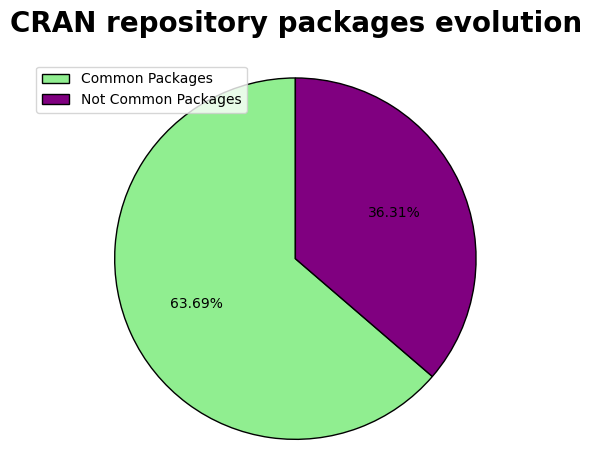
\includegraphics[width=0.7\textwidth]{img/cran/circle.png}
        \caption{Comparacion de los paquetes comunes entre los dos conjuntos de datos.}
        \label{fig:cran_common_packages2}
    \end{center}
\end{figure}

\begin{figure}[h!]
    \begin{center}
        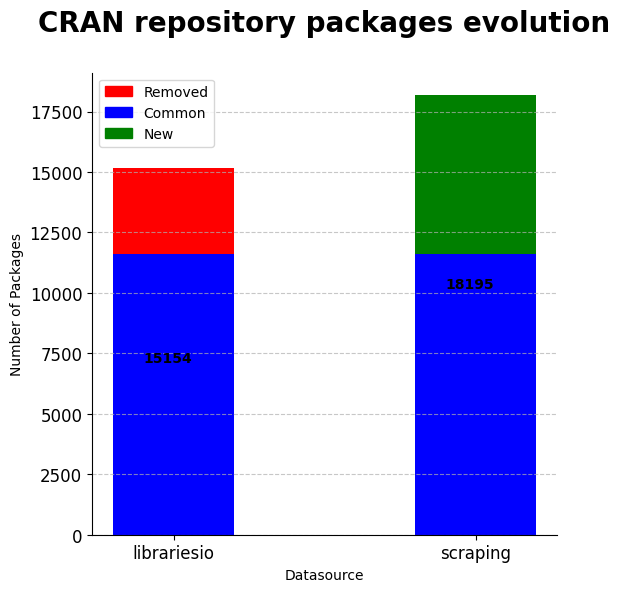
\includegraphics[width=0.6\textwidth]{img/cran/bars.png}
        \caption{Comparacion del numero de paquetes.}
        \label{fig:cran_common_packages3}
    \end{center}
\end{figure}

Por consiguiente, se concluye que el conjunto de datos \textit{scraped} proporciona una
visión más completa y actualizada de los paquetes disponibles. Al incluir tanto los paquetes
en común como los paquetes adicionales respecto a \textit{libraries.io}, \textit{scraped}
se configura como una fuente valiosa para investigaciones y análisis en el ámbito de estudio.






\subsection{El tamaño}

A continuacion realizaremos una comparacion de las medidas de tamaño entre los dos conjuntos de datos y como es
el agrupamiento de los nodos en cada uno de ellos. \ref{tab:cran_size}

\begin{table}[h!]
    \begin{center}
        \begin{tabular}{|l|c|c|c|}
            \hline
            \textbf{Medida}                & \textbf{libraries.io} & \textbf{scraped} \\
            \hline
            Number of nodes                & 15647                 & 18671            \\
            Number of edges                & 76207                 & 113273           \\
            Average degree                 & 9.740                 & 12.133           \\
            Average clustering coefficient & 0.131                 & 0.152            \\
            \hline
        \end{tabular}
        \caption{Comparación de medidas de tamaño entre los dos conjuntos de datos.}
        \label{tab:cran_size}
    \end{center}
\end{table}

La red \textit{scraped} tiene un mayor número de nodos (\textit{18671}) en comparación con la
red \textit{libraries.io} (\textit{15647}). Esto indica que \textit{scraped} contiene más elementos o entidades
interconectadas en su estructura de red.

La red \textit{scraped} también tiene un mayor número de aristas o enlaces (\textit{113273}) en
comparación con la red \textit{libraries.io} (\textit{76207}). Esto implica que \textit{scraped} tiene más
conexiones entre los nodos, lo que aumenta su grado de conectividad.

El grado promedio de los nodos en la red \textit{scraped} es más alto (\textit{12.133}) en
comparación con el de la red \textit{libraries.io} (\textit{9.740}). Esto sugiere que, en promedio, cada nodo
en \textit{scraped} tiene más conexiones con otros nodos en comparación con los nodos en \textit{libraries.io}.

El coeficiente de agrupamiento promedio en la red \textit{scraped} es
ligeramente más alto (\textit{0.152}) que en la red \textit{libraries.io} (\textit{0.131}). Esto indica que,
en promedio, los nodos en \textit{scraped} tienen una mayor tendencia a formar grupos o comunidades más densamente
interconectadas en comparación con los nodos en \textit{libraries.io}.

\subsection{El grado}

\begin{figure}[h!]
    \begin{center}
        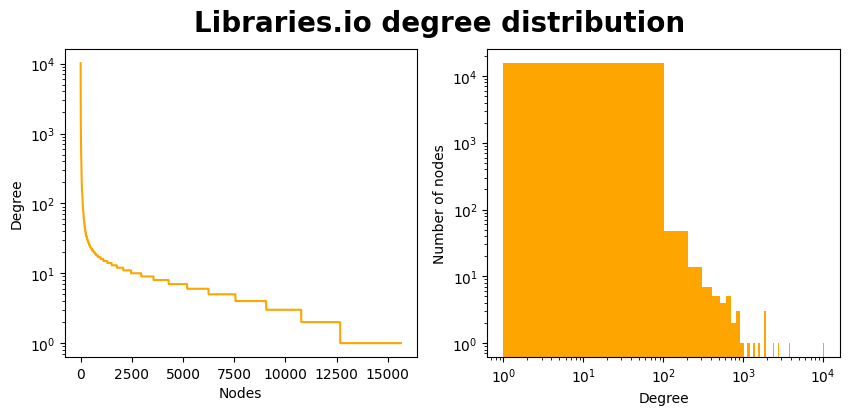
\includegraphics[width=1\textwidth]{img/cran/distribucion_grado.png}
        \caption{Distribucion de grado \textit{libraries.io}.}
        \label{fig:cran_degree_distribution}
    \end{center}
\end{figure}

\begin{figure}[h!]
    \begin{center}
        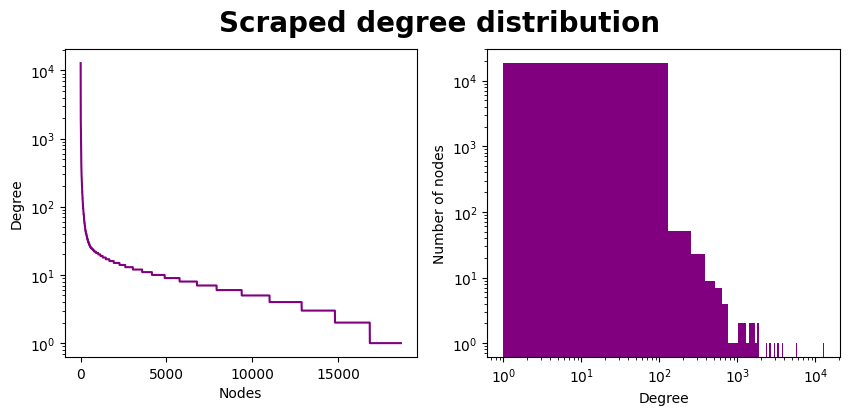
\includegraphics[width=1\textwidth]{img/cran/distribucion_grado2.png}
        \caption{Distribucion de grado \textit{scraped}.}
        \label{fig:cran_degree_distribution_scraped}
    \end{center}
\end{figure}

Al realizar una comparativa de las distribuciones de grado entre ambos conjuntos de datos,
se evidencia un leve incremento en el grado promedio. El grado promedio del conjunto de datos
\textit{libraries.io} es de 4.87, mientras que en el conjunto \textit{scraped} alcanza un valor
de 6.06. Estos resultados indican un incremento en la conectividad y la relevancia de los
paquetes más destacados en el conjunto de datos \textit{scraped}. Tal variación en los valores
promedio refleja el aumento en la importancia y la interconexión de los paquetes dentro de este
conjunto de datos, lo cual puede estar relacionado con su mayor tamaño y actualización.
\ref{fig:cran_degree_distribution} \ref{fig:cran_degree_distribution_scraped}

Además, se observa que la tendencia a disminuir el número de dependencias es ligeramente
más pronunciada que la tendencia a aumentarlas. Esto sugiere que, en la evolución de
la red de dependencias, los paquetes tienden a reducir su dependencia directa o a
reorganizar sus conexiones con otros paquetes, lo que puede ser resultado de procesos
de \textit{refactorización}, \textit{optimización} o \textit{consolidación}.


\subsubsection{Grado de salida (\textit{out degree})}


En el análisis de la distribución del grado de salida, no se observan diferencias significativas
que puedan ser comparadas. Podemos inferir que ambas distribuciones siguen una tendencia
similar, con la única distinción de que en el conjunto de datos nuevo se encuentra un mayor
número de nodos \ref{fig:cran_out_lib} \ref{fig:cran_out_scraped}.

\begin{figure}[h!]
    \begin{center}
        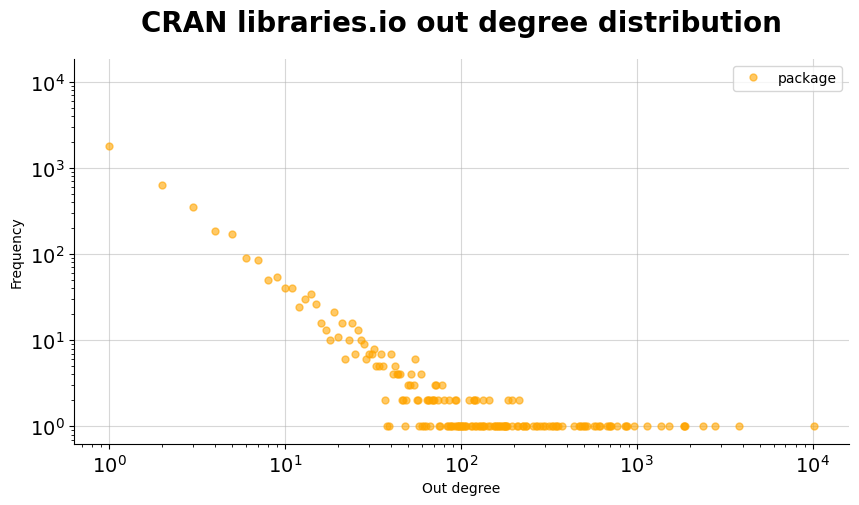
\includegraphics[width=1\textwidth]{img/cran/out_deg.png}
        \caption{Distribucion de Out degree de \textit{libraries.io}.}
        \label{fig:cran_out_lib}
    \end{center}
\end{figure}

\begin{figure}[h!]
    \begin{center}
        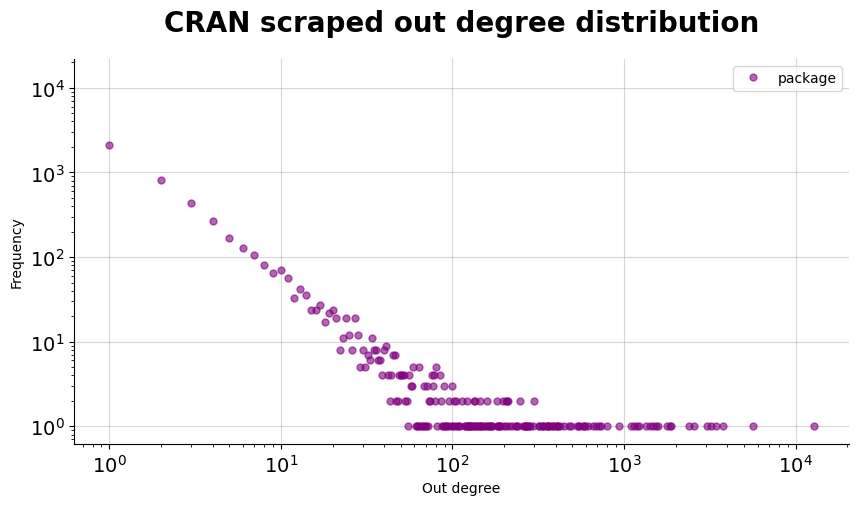
\includegraphics[width=1\textwidth]{img/cran/out_deg2.png}
        \caption{Distribucion de Out degree de \textit{scraped}.}
        \label{fig:cran_out_scraped}
    \end{center}
\end{figure}

Al examinar el conjunto de paquetes con mayor grado de salida, se observa un aumento generalizado
en todos ellos. Estos paquetes destacados representan una centralidad de grado significativa,
lo que implica que son las dependencias más utilizadas dentro del sistema. Es comprensible que
estos paquetes, al ser ampliamente utilizados, hayan mantenido una presencia constante en la
red y hayan experimentado un incremento en el número de sus dependientes debido al surgimiento
de nuevos paquetes. \ref{fig:cran_out_libio_top}

\begin{figure}[h!]
    \begin{center}
        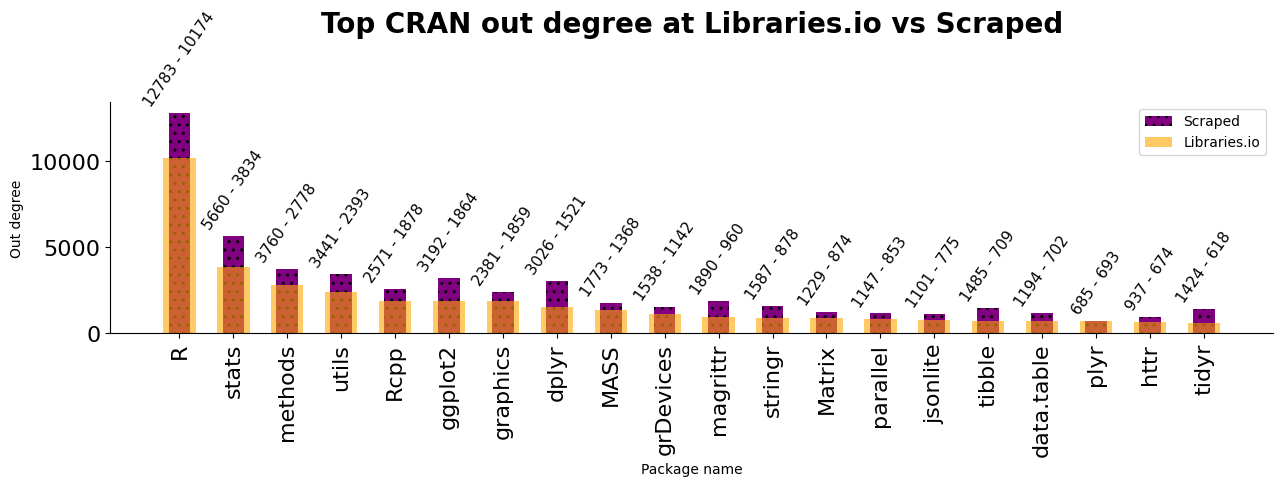
\includegraphics[width=1\textwidth]{img/cran/out_lib.png}
        \caption{Top paquetes con mayor grado de salida en \textit{libraries.io}.}
        \label{fig:cran_out_libio_top}
    \end{center}
\end{figure}

Esta observación refuerza la importancia y la relevancia de estos paquetes clave en el
ecosistema estudiado. Su estabilidad y el aumento en sus dependientes pueden atribuirse a
su funcionalidad y a su amplia adopción por parte de los usuarios. Además, el incremento en
la cantidad de dependientes es un indicativo del crecimiento y la evolución continua del
sistema, donde se generan nuevas relaciones de dependencia entre los paquetes existentes
y los recién agregados.

Al realizar la comparativa utilizando el nuevo conjunto de datos, se observa que los principales
representantes del ranking se mantienen presentes. Sin embargo, se han producido algunas variaciones
en el orden de algunos puestos dentro del top. Además, se ha registrado la inclusión de paquetes que
previamente se encontraban fuera del top. \ref{fig:cran_out_scraped_top}

\begin{figure}[h!]
    \begin{center}
        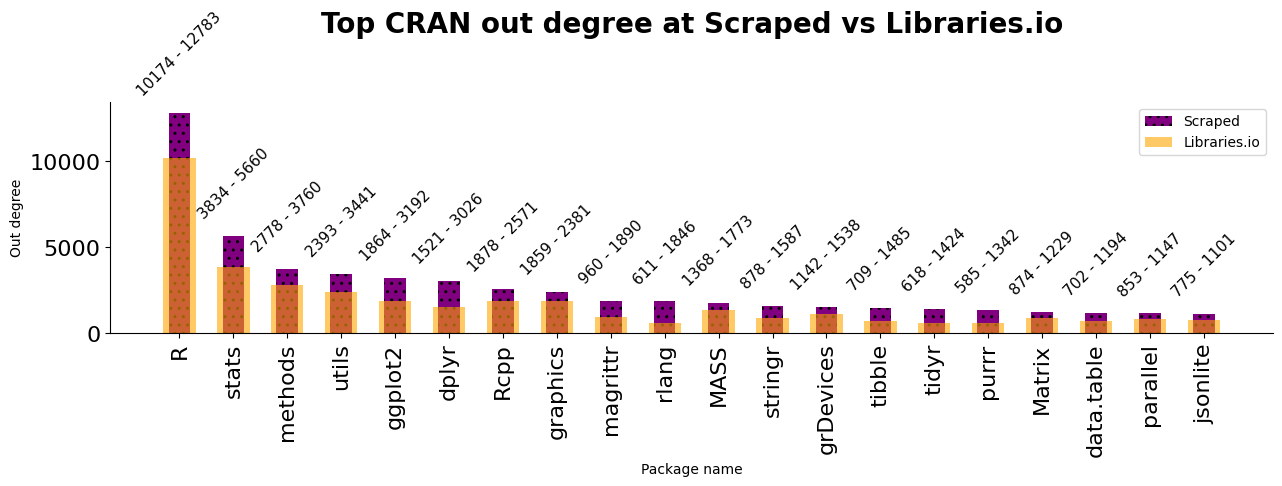
\includegraphics[width=1\textwidth]{img/cran/out_scr.png}
        \caption{Top paquetes con mayor grado de salida en \textit{scraped}.}
        \label{fig:cran_out_scraped_top}
    \end{center}
\end{figure}

Esta inclusión de paquetes puede atribuirse al incremento en el número de sus dependencias,
el cual ha superado a aquellos que han salido del top en este periodo de tiempo analizado.
Estos nuevos paquetes han logrado adquirir una mayor relevancia y han fortalecido su posición
dentro del conjunto de datos. Este fenómeno puede ser consecuencia de su creciente adopción y
de la expansión de su funcionalidad, lo que ha llevado a un incremento en el número de paquetes
que los utilizan como dependencias.

Este incremento lo podemos ver reprensentado en la siguiente figura \ref{fig:cran_dependents_dist}.

\begin{figure}[h!]
    \begin{center}
        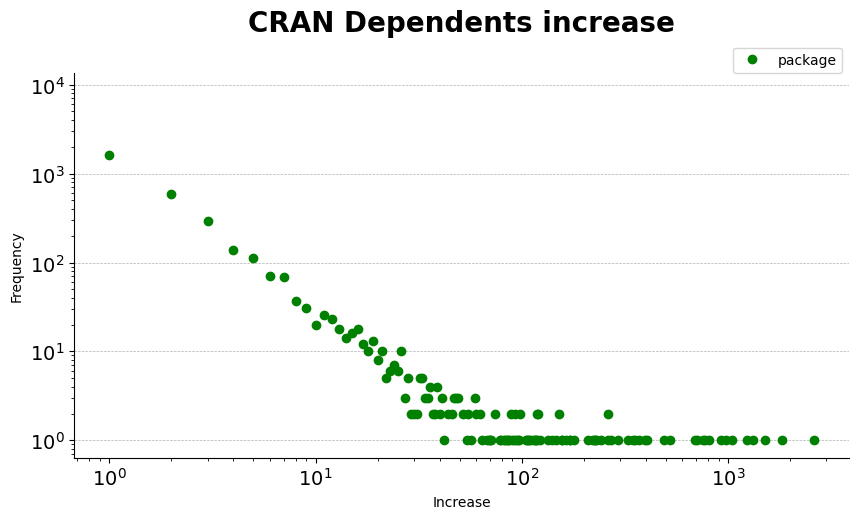
\includegraphics[width=1\textwidth]{img/cran/dependents_dist.png}
        \caption{Distribucion de dependientes.}
        \label{fig:cran_dependents_dist}
    \end{center}
\end{figure}

\subsubsection{Grado de entrada (\textit{in degree})}


En el análisis de la distribución del grado de entrada, se observa un comportamiento común
en ambos conjuntos de datos. Debido a su similitud, resulta difícil extraer conclusiones
significativas. Sin embargo, se puede observar un ligero incremento en el nuevo conjunto de
datos en comparación con el conjunto de datos de libraries.io. \ref{fig:cran_in_lib} \ref{fig:cran_in_scraped}

\begin{figure}[h!]
    \begin{center}
        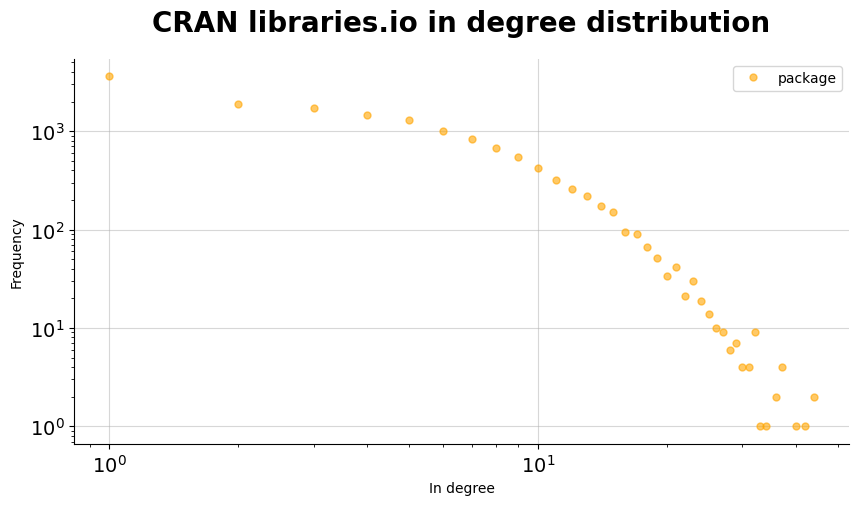
\includegraphics[width=0.8\textwidth]{img/cran/ind_lib.png}
        \caption{Distribucion de In degree de \textit{libraries.io}.}
        \label{fig:cran_in_lib}
    \end{center}
\end{figure}

\begin{figure}[h!]
    \begin{center}
        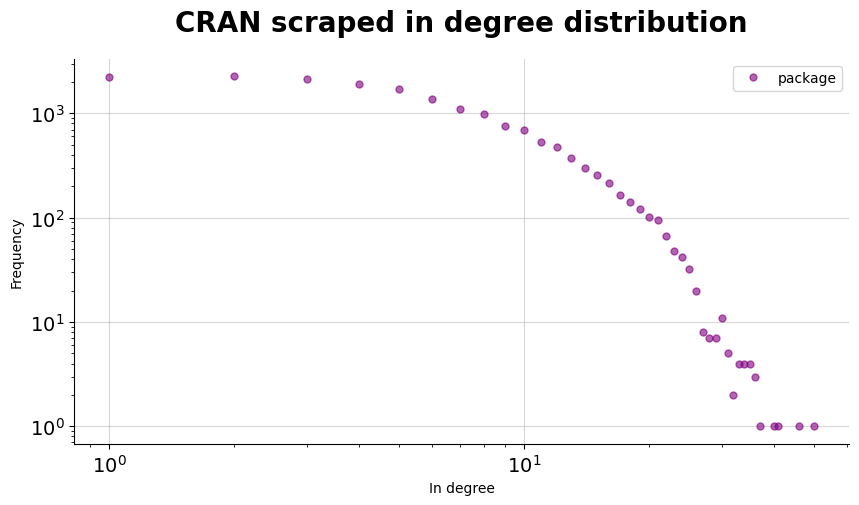
\includegraphics[width=0.8\textwidth]{img/cran/ind_scr.png}
        \caption{Distribucion de In degree de \textit{scraped}.}
        \label{fig:cran_in_scraped}
    \end{center}
\end{figure}

Tomando como punto de referencia la frecuencia de nodos con un grado de entrada de valor 20,
en el conjunto de datos de libraries.io se encuentran alrededor de 50 nodos, mientras que en
el nuevo conjunto de datos se registran aproximadamente 100 nodos. Estos valores pueden sugerir
un aumento en la cantidad de paquetes que reciben un número determinado de dependencias.


Si representamos el \textit{top} de \textit{in degree} de los paquetes del conjunto de datos
de \textit{libraries.io}, podemos identificar aquellos paquetes que poseen un mayor número de
dependencias. Estos paquetes podrían considerarse los más vulnerables en su primer nivel de dependencia,
sin tener en cuenta la transitividad. Al analizar los resultados, se puede concluir que un porcentaje
significativo de los paquetes destacados en este \textit{top} han mantenido su presencia en la red a
lo largo del tiempo.

Además, se observa una tendencia general a disminuir el número de dependencias para la mayoría de
los casos en el \textit{top}. Esto sugiere que, a medida que evoluciona la red de dependencias,
algunos paquetes han logrado reducir su dependencia directa o han redistribuido sus conexiones
con otros paquetes.


\begin{figure}[h!]
    \begin{center}
        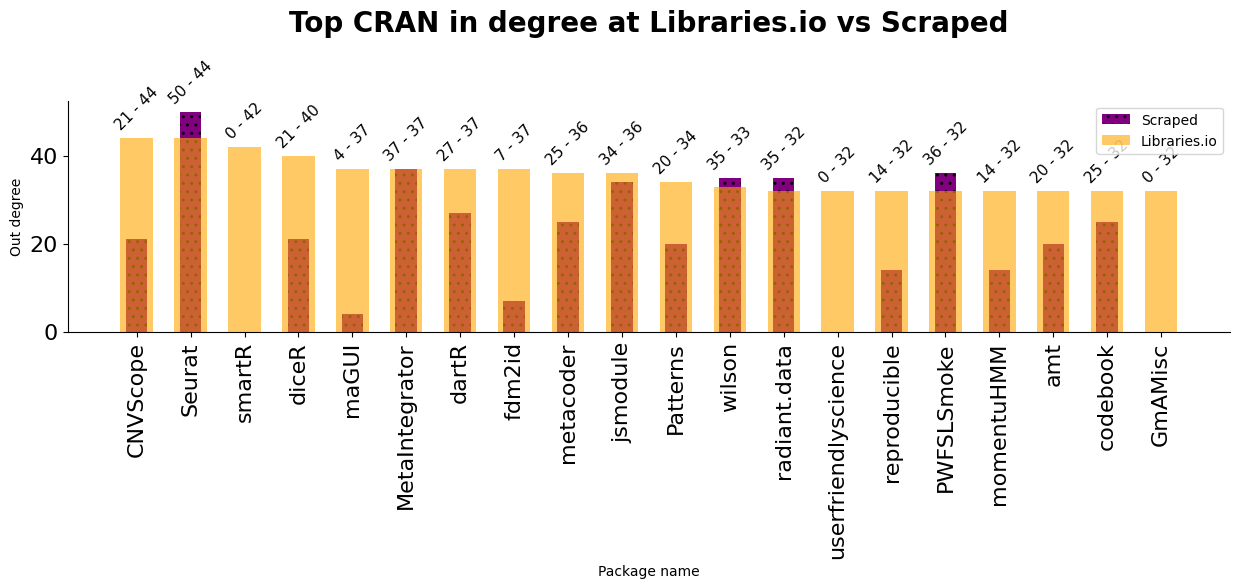
\includegraphics[width=1\textwidth]{img/cran/top_ind_libio.png}
        \caption{Top paquetes con mayor grado de entrada en \textit{libraries.io}.}
        \label{fig:top_ind_libio_cran}
    \end{center}
\end{figure}


Desde la perspectiva del \textit{top} de \textit{in degree}, se observa una notable variación en
la evolución de los paquetes. Aproximadamente la mitad de los individuos que conformaban el
\textit{top} han sido reemplazados. Estos paquetes de reemplazo se caracterizan por ser nuevos
en la red, lo cual sugiere que están utilizando funcionalidades previamente desarrolladas para
generar nuevas capacidades.

Es común que aparezcan nuevos paquetes en este \textit{top}, dado el contexto de una red de
carácter científico. A medida que el software madura, es habitual que estos paquetes más
jóvenes se refactoricen con el tiempo, tendiendo a disminuir sus dependencias.

Por otro lado, existen paquetes que no solo se encontraban en el \textit{top} anterior,
sino que han incrementado sus dependencias. Este aumento puede ser indicativo de paquetes
cuya funcionalidad aún está en desarrollo y continúa evolucionando. \ref{fig:top_ind_scraped_cran}

\begin{figure}[h!]
    \begin{center}
        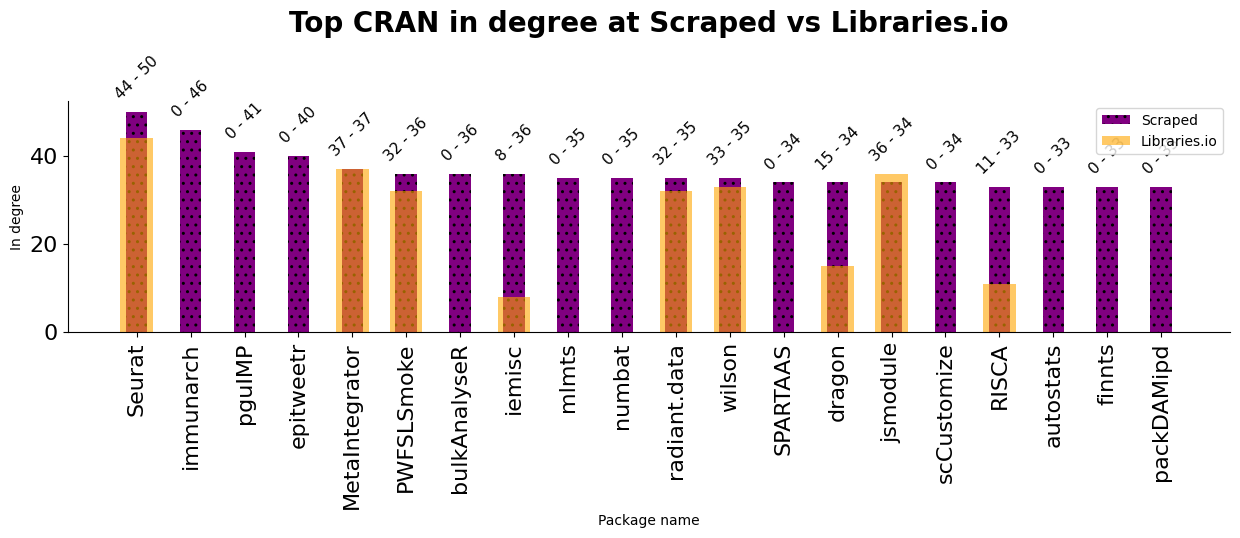
\includegraphics[width=1\textwidth]{img/cran/top_ind_scraped.png}
        \caption{Top paquetes con mayor grado de entrada en \textit{scraped}.}
        \label{fig:top_ind_scraped_cran}
    \end{center}
\end{figure}


Al observar la tendencia del incremento de dependencias en la red, se evidencia que, en
general, es común que el número de dependencias de los paquetes no experimente cambios
drásticos. La mayoría de los paquetes se sitúan en un rango de incremento de dependencias
de aproximadamente $\pm$10. \ref{fig:cran_dependencies_increase}


\begin{figure}[h!]
    \begin{center}
        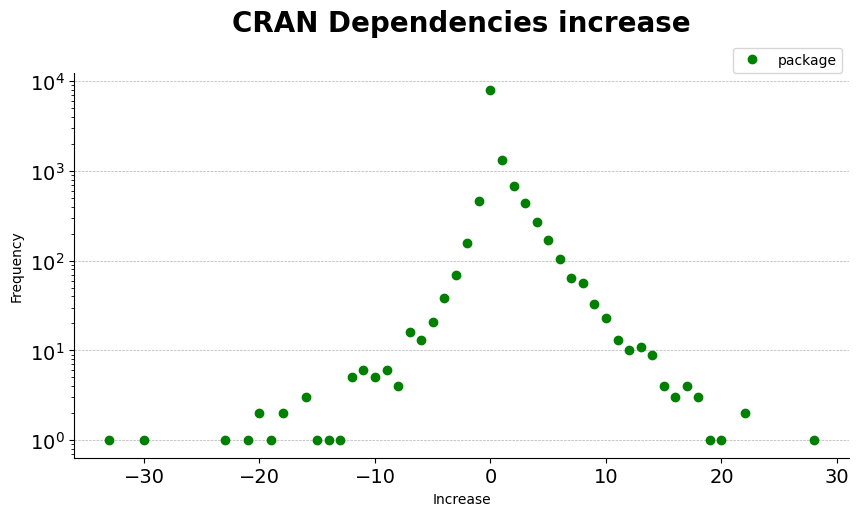
\includegraphics[width=1\textwidth]{img/cran/dependencies_increase.png}
        \caption{Incremento de dependencias.}
        \label{fig:cran_dependencies_increase}
    \end{center}
\end{figure}

\subsection{El \textit{PageRank}}

A partir del análisis de la distribución de \textit{PageRank} en la red, se observa la presencia
de numerosos nodos con un \textit{PageRank} bajo, y a medida que se incrementa el valor del
\textit{PageRank}, la frecuencia de nodos disminuye gradualmente. Este patrón revela la
existencia de muchos nodos de baja importancia en la red, junto con un grupo reducido de
paquetes que son considerados importantes debido a sus dependencias, las cuales, a su vez,
son también dependencias relevantes en la red.

Al comparar las dos distribuciones, se aprecia una diferencia notable en la red
de \textit{libraries.io}, donde el valor máximo alcanzado por el \textit{PageRank} de
un paquete es mayor en comparación con la nueva red. Esta diferencia puede interpretarse
como un indicio de que, en la evolución de \textit{CRAN}, los paquetes más importantes
se han estabilizado, mientras que han surgido otros paquetes que están adquiriendo
relevancia. Como resultado, el \textit{PageRank} se ha distribuido de manera más equitativa
entre los paquetes de la red. \ref{fig:cran_pr_libio} \ref{fig:cran_pr_scraped}

\begin{figure}[h!]
    \begin{center}
        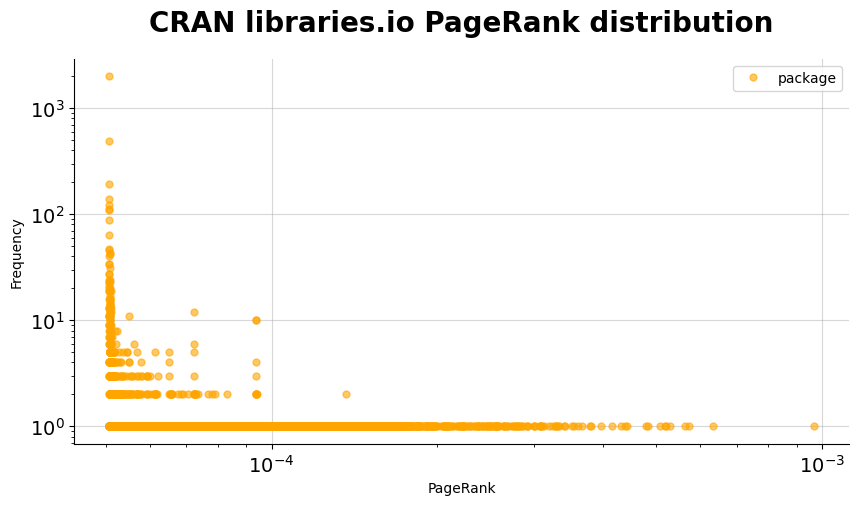
\includegraphics[width=1\textwidth]{img/cran/pr.png}
        \caption{Distribucion de \textit{PageRank} en \textit{libraries.io}.}
        \label{fig:cran_pr_libio}
    \end{center}
\end{figure}

\begin{figure}[h!]
    \begin{center}
        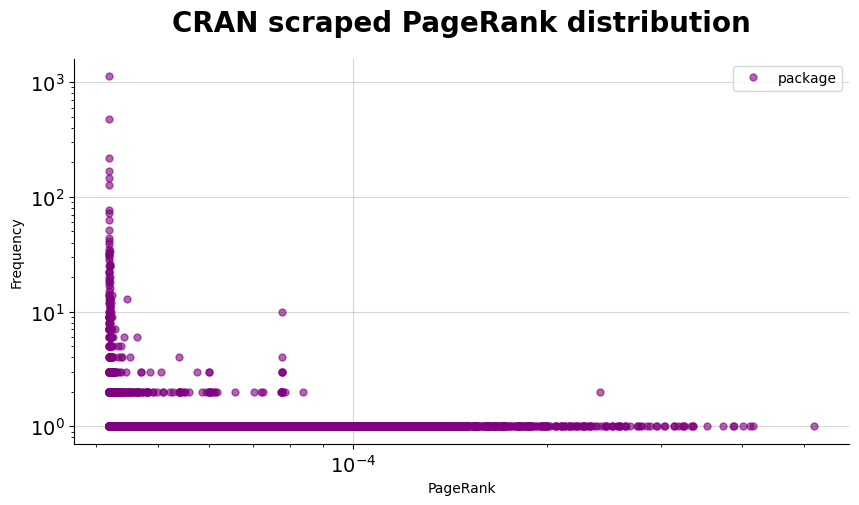
\includegraphics[width=1\textwidth]{img/cran/pr2.png}
        \caption{Distribucion de \textit{PageRank} en \textit{scraped}.}
        \label{fig:cran_pr_scraped}
    \end{center}
\end{figure}

El top de mayor \textit{PageRank} en \textit{libraries.io} nos brinda una visión de los paquetes que se
consideran como nodos centrales en la red de dependencias. Esto implica que son elementos fundamentales
para la funcionalidad y el rendimiento de otros paquetes, dado que poseen un mayor número de dependencias
directas e indirectas.

Estos paquetes tienden a ser dependientes de otros paquetes con alto \textit{PageRank}. Además, desde el
punto de vista de la vulnerabilidad, son considerados críticos debido a que suelen acumular una alta
dependencia transitiva. Esto significa que cualquier cambio o problema en estos paquetes centrales puede
tener un impacto significativo en todo el ecosistema de la red de dependencias.

Estos nodos de alto \textit{PageRank} juegan un papel crucial en el mantenimiento y la estabilidad de la
red de dependencias. Su importancia radica en su alta interconexion con otros paquetes similares. \ref{fig:cran_pr_libio_top}

\begin{figure}[h!]
    \begin{center}
        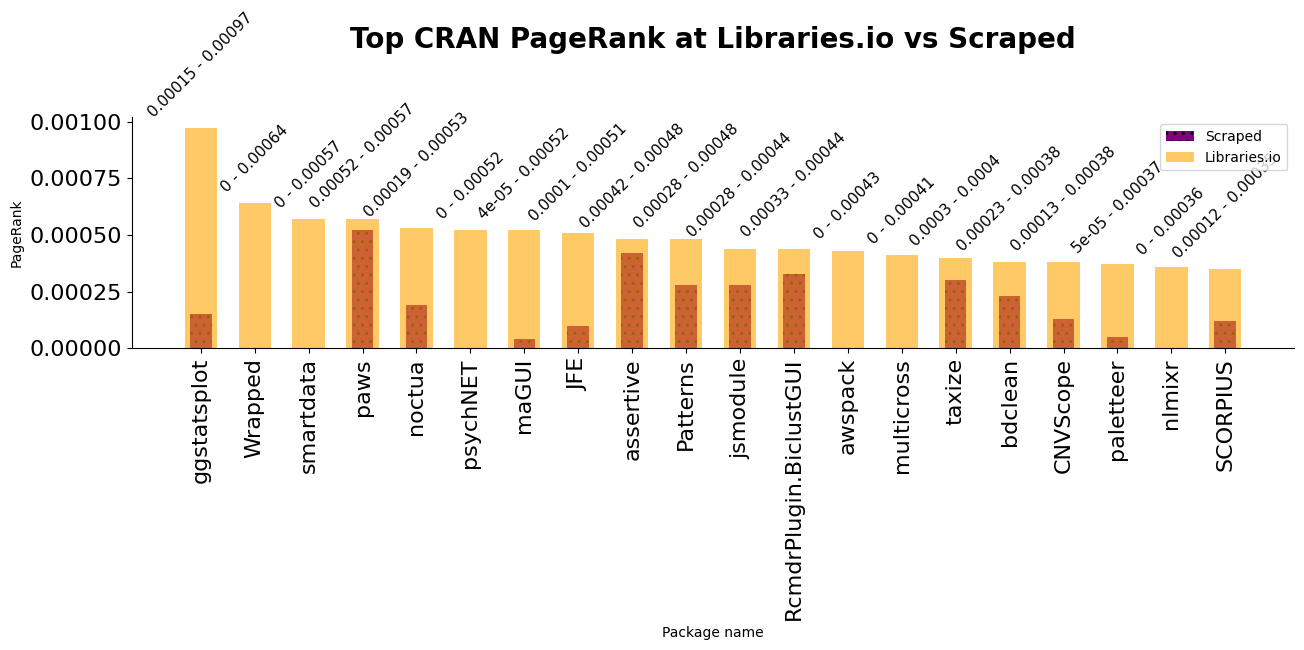
\includegraphics[width=1\textwidth]{img/cran/pr_top.png}
        \caption{Top \textit{PageRank} en \textit{libraries.io}.}
        \label{fig:cran_pr_libio_top}
    \end{center}
\end{figure}



En base a la introducción anterior, es esperable encontrar paquetes en el top de \textit{libraries.io}
que no estén presentes en el conjunto de datos de \textit{scraped}.

\begin{figure}[h!]
    \begin{center}
        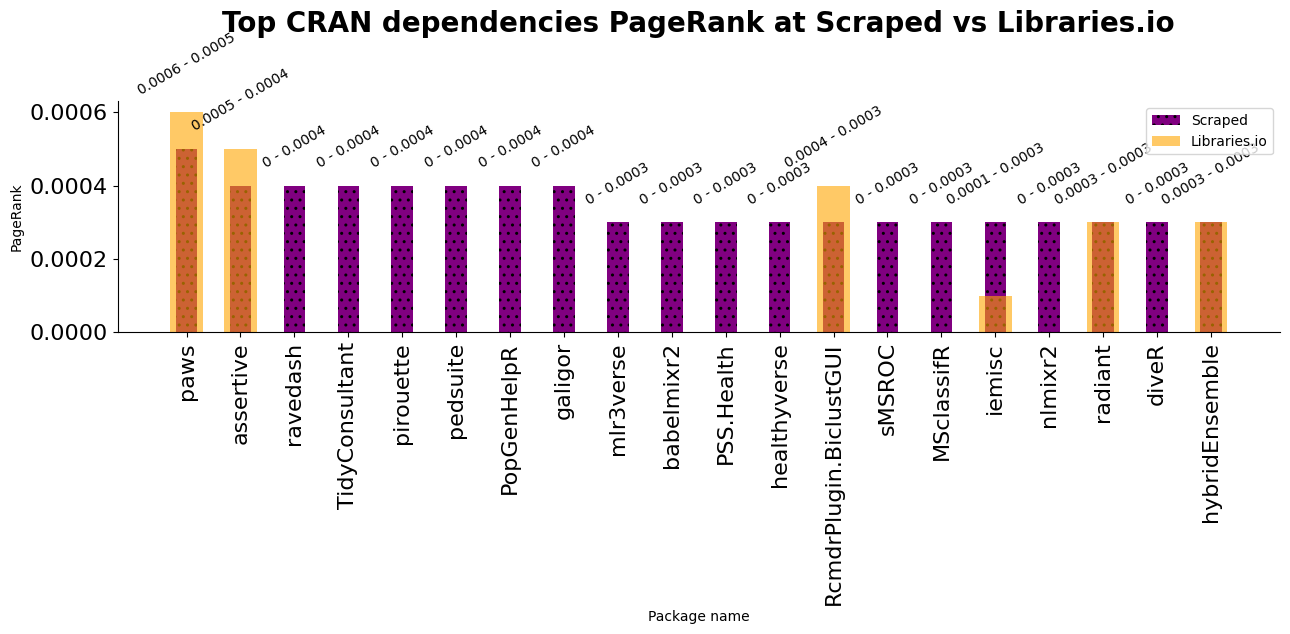
\includegraphics[width=1\textwidth]{img/cran/pr_top2.png}
        \caption{Top \textit{PageRank} en \textit{scraped}.}
        \label{fig:cran_pr_scraped_top}
    \end{center}
\end{figure}

A partir del nuevo conjunto de datos \ref{fig:cran_pr_scraped_top}, se observa un descenso general en los
valores de PageRank en comparación con el conjunto de datos de \textit{libraries.io}. Además, se destaca
que un gran número de paquetes han ingresado al top de PageRank y no estaban presentes en \textit{libraries.io}.
Este hallazgo refuerza la teoría de que el PageRank, en el contexto de una red de dependencias, puede
considerarse un indicador de la vulnerabilidad de un paquete. Se puede inferir que estos paquetes recién
incorporados tienden a tener una presencia transitoria en la red y, debido a su relativa falta de madurez,
es probable que experimenten variaciones significativas a lo largo del tiempo.

Sin embargo, resulta más interesante centrar la atención en aquellos paquetes que mantienen un alto valor de
PageRank a lo largo del tiempo. Estos paquetes indican la presencia de dependencias importantes y altamente
transitivas en la red, lo que los hace potencialmente más vulnerables. Su capacidad para conservar su
importancia en el contexto de la evolución de la red sugiere que desempeñan un papel fundamental en el
funcionamiento y la estabilidad de otros paquetes. \ref{fig:Top 20 PageRank numero de dependencias transitivas en libraries.io}
\ref{fig:Top 20 PageRank numero de dependencias transitivas en scraped}

\begin{figure}[h!]
    \begin{center}
        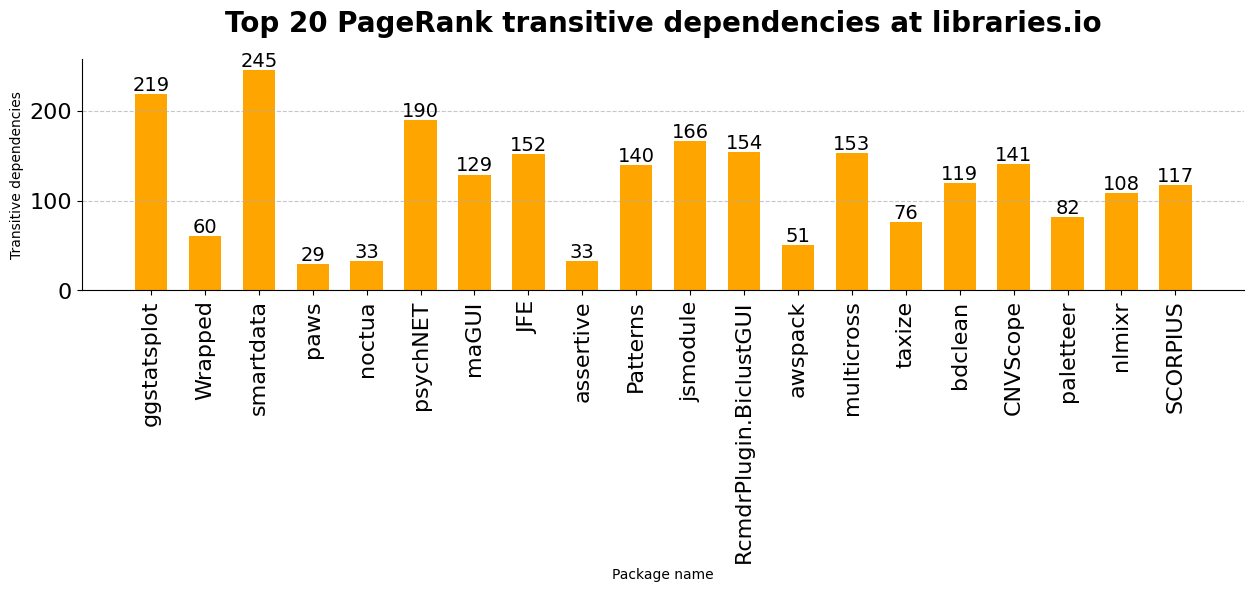
\includegraphics[width=1\textwidth]{img/cran/pr_trans.png}
        \caption{Top 20 \textit{PageRank} numero de dependencias transitivas en libraries.io}
        \label{fig:Top 20 PageRank numero de dependencias transitivas en libraries.io}
    \end{center}
\end{figure}

\begin{figure}[h!]
    \begin{center}
        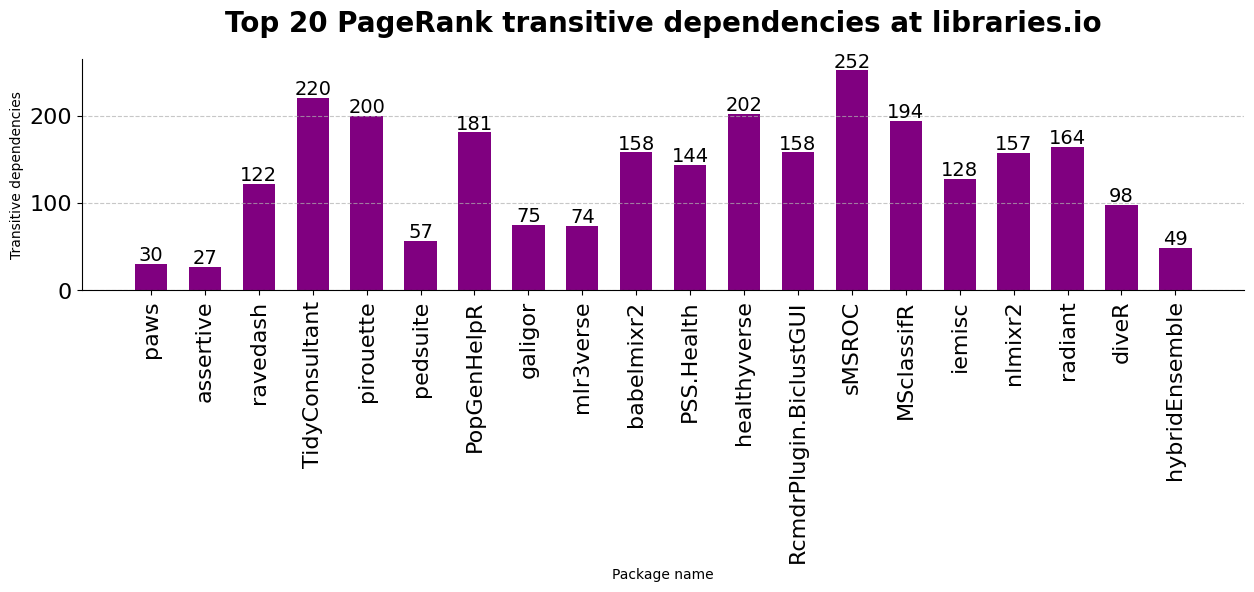
\includegraphics[width=1\textwidth]{img/cran/pr_trans2.png}dependidos
        \caption{Top 20 \textit{PageRank} numero de dependencias transitivas en scraped}
        \label{fig:Top 20 PageRank numero de dependencias transitivas en scraped}
    \end{center}
\end{figure}

Desde una perspectiva inversa, el uso del \textit{PageRank} nos permite identificar qué paquetes son dependencia
de otros paquetes importantes en la red de dependencias. Esto proporciona una visión de
la centralidad en términos de popularidad de un paquete. Al analizar el \textit{PageRank} bajo esta perspectiva, es
posible determinar qué paquetes son altamente requeridos por otros paquetes y, por lo tanto,
desempeñan un papel crucial en el funcionamiento de la red. \ref{fig:Top 20 PageRank paquetes en sraped}

\begin{figure}[h!]
    \begin{center}
        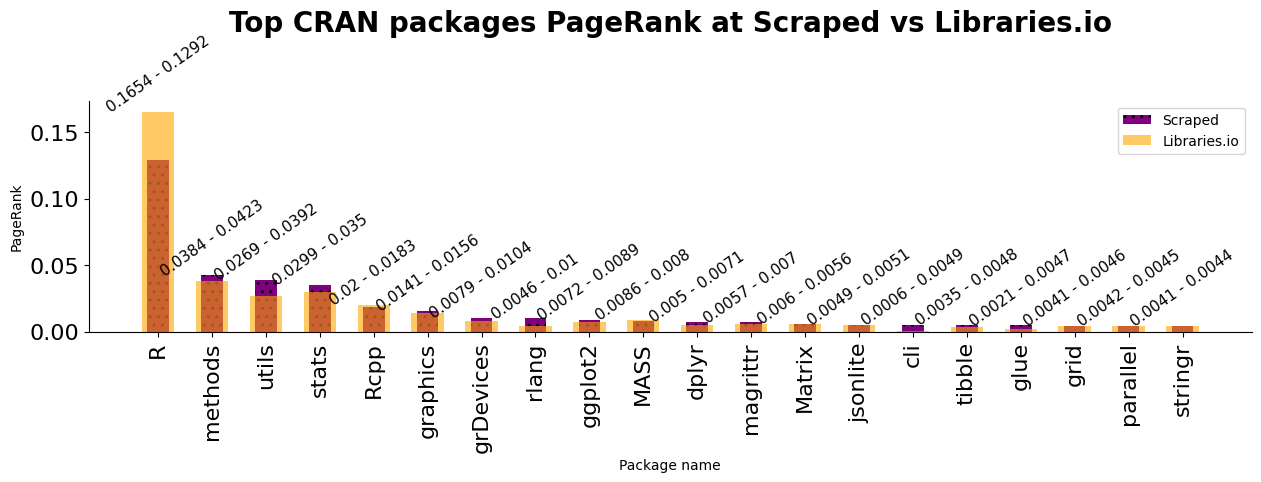
\includegraphics[width=1\textwidth]{img/cran/pr_inverted.png}
        \caption{Top 20 \textit{PageRank} paquetes en sraped}
        \label{fig:Top 20 PageRank paquetes en sraped}
    \end{center}
\end{figure}

Los paquetes mostrados en este top son los mas populares del ecosistema de \textit{R}.
Estos paquetes son los mas utilizados por otros paquetes, lo que los hace fundamentales para el
funcionamiento de la red de dependencias. No es raro que el paquete R, que implementa el \textit{core}
del lenguaje, sea el paquete mas popular.

\begin{figure}[h!]
    \begin{center}
        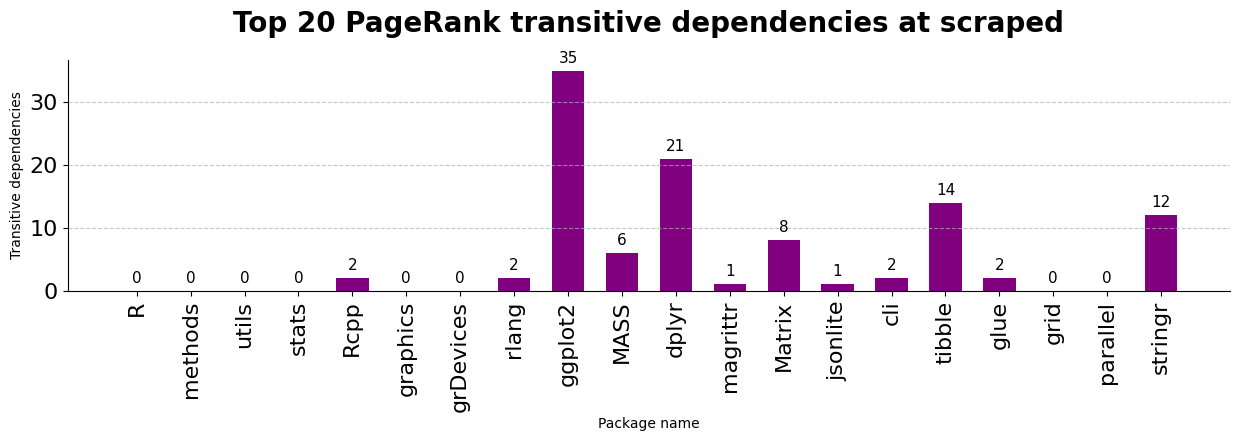
\includegraphics[width=1\textwidth]{img/cran/transitive_pr_scr.png}
        \caption{Top 20 \textit{PageRank} paquetes numero de dependencias transitivas en sraped}
        \label{fig:Top 20 PageRank paquetes numero de dependencias transitivas en sraped}
    \end{center}
\end{figure}

Estos paquetes a nivel de vulnerabilidad son los mas estables, ya que el numero de dependencias
transitivas que tienen es relativamente bajo. \ref{fig:Top 20 PageRank paquetes numero de dependencias transitivas en sraped}

\subsection{Impacto (\textit{Impact})}

Desde el punto de vista de esta metrica, podemos interpretar la vulnerabilidad de un paquete como el numero
de dependencias paquetes que se ven afectados por un cambio en el paquete. En este sentido, un paquete
vulnerable es aquel que tiene un alto impacto en la red de dependencias.

\begin{figure}[h!]
    \begin{center}
        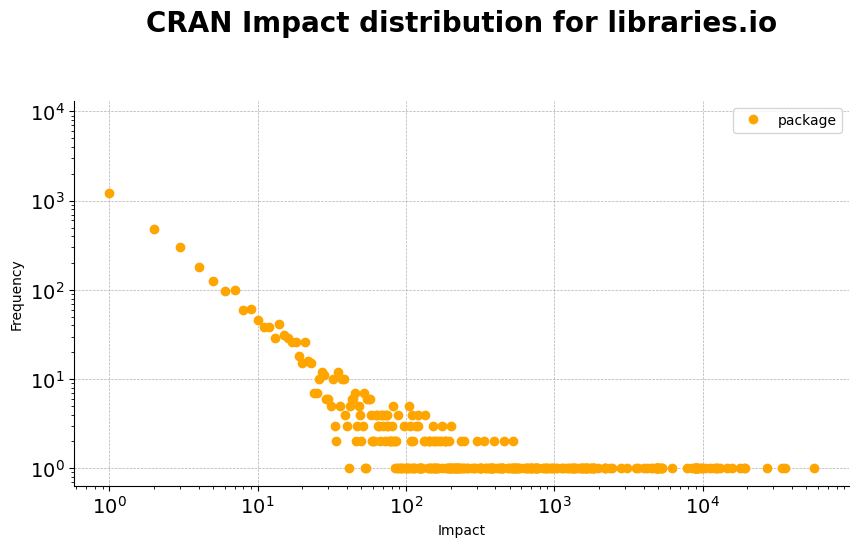
\includegraphics[width=0.8\textwidth]{img/cran/impact_dist_libio.png}
        \caption{Distribución de \textit{Impact} en libraries.io}
        \label{fig:Distribución de Impact en libraries.io}
    \end{center}
\end{figure}

\begin{figure}[h!]
    \begin{center}
        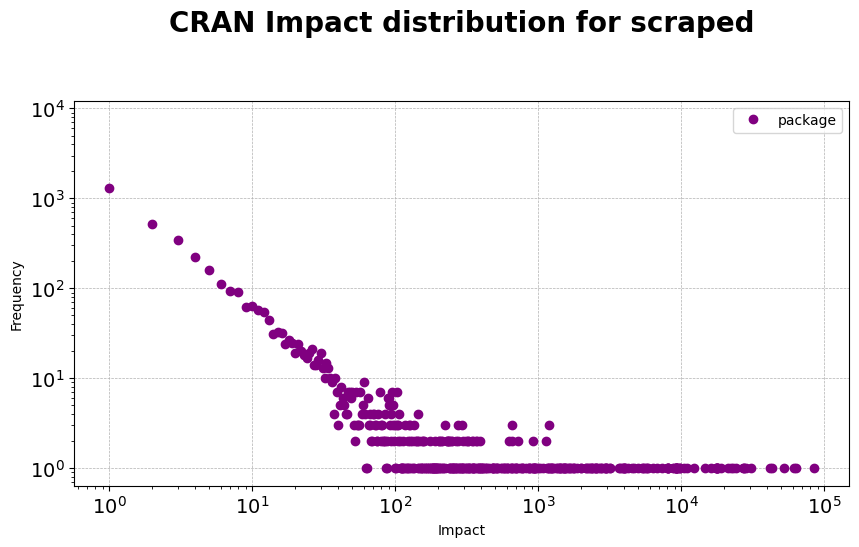
\includegraphics[width=0.8\textwidth]{img/cran/impact_dist_scraped.png}
        \caption{Distribución de \textit{Impact} en scraped}
        \label{fig:Distribución de Impact en scraped}
    \end{center}
\end{figure}

A partir del análisis de la distribución del impacto, se observa una tendencia similar en ambos
conjuntos de datos. Se aprecia un ligero incremento en el impacto en el nuevo conjunto de datos,
pero en general los valores se mantienen estables. Este incremento puede atribuirse a la incorporación
de nuevos paquetes en la red, los cuales han adoptado dependencias existentes, lo que ha aumentado el
impacto de estas últimas. \ref{fig:Distribución de Impact en libraries.io} \ref{fig:Distribución de Impact en scraped}


En el top de paquetes con mayor \textit{impacto} se encuentran aquellos que son considerados los más populares
en la red, en términos de su influencia sobre otros paquetes. Es notable que los principales representantes
de este top también aparecen en el top del \textit{PageRank} a nivel de la red de paquetes. Desde el punto
de vista de la \textit{dependencia transitiva}, estos paquetes son aquellos que tienen la mayor cantidad de
dependientes en toda la red.

Al analizar el \textit{impacto} de estos paquetes, se observa un aumento en su valor, en algunos casos
significativo. Esto indica que estos paquetes han demostrado ser estables en el tiempo y en su implementación,
y que su funcionalidad es altamente útil para la red.

\begin{figure}[h!]
    \begin{center}
        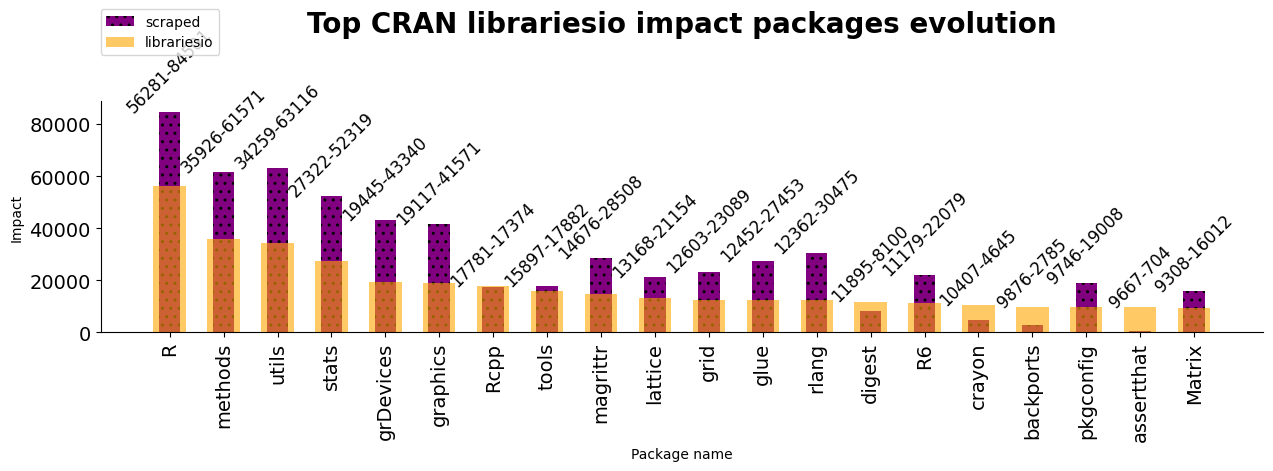
\includegraphics[width=1\textwidth]{img/cran/impact_top_libio.png}
        \caption{Top paquetes con mayor \textit{Impact} en libraries.io}
        \label{fig:Top impact libraries.io}
    \end{center}
\end{figure}

\begin{figure}[h!]
    \begin{center}
        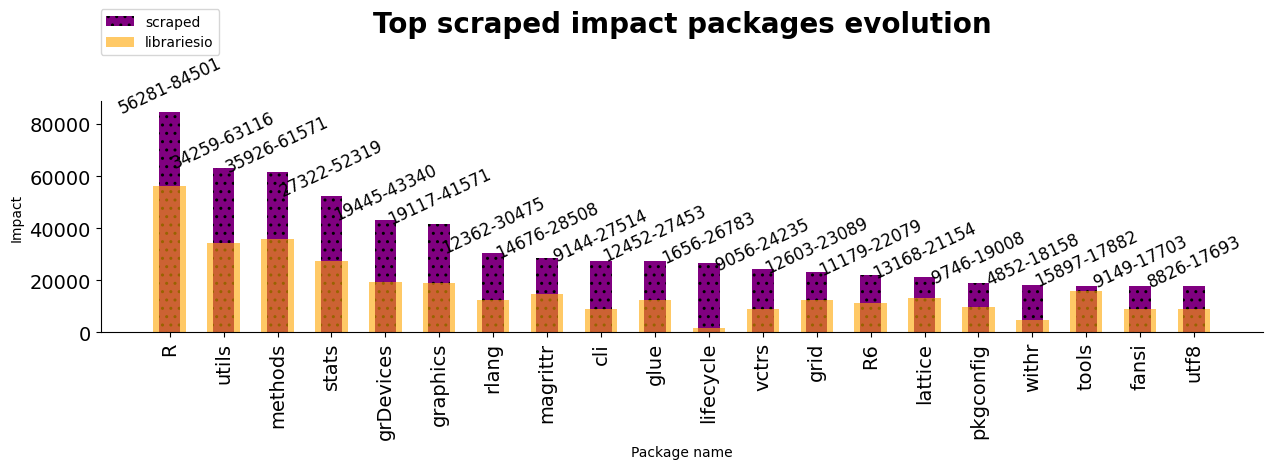
\includegraphics[width=1\textwidth]{img/cran/impact_top_scraped.png}
        \caption{Top paquetes con mayor \textit{Impact} en scraped}
        \label{fig:Top impact scraped}
    \end{center}
\end{figure}

Por otro lado, aquellos paquetes en el top que han experimentado una reducción en su \textit{impacto}
podrían indicar la aparición de otros paquetes con funcionalidades similares o mejoradas, los cuales han
sido elegidos como alternativas por los usuarios de la red. \ref{fig:Top impact libraries.io} \ref{fig:Top impact scraped}

\begin{table}[h!]
    \begin{center}
        \begin{tabular}{|l|r|r|r|}
            \hline
            \textbf{Package} & \textbf{libraries.io} & \textbf{scraped} & \textbf{increment} \\
            \hline
            utils            & 34259                 & 63116            & 28857              \\
            R                & 56281                 & 84501            & 28220              \\
            methods          & 35926                 & 61571            & 25645              \\
            lifecycle        & 1656                  & 26783            & 25127              \\
            stats            & 27322                 & 52319            & 24997              \\
            grDevices        & 19445                 & 43340            & 23895              \\
            graphics         & 19117                 & 41571            & 22454              \\
            cli              & 9144                  & 27514            & 18370              \\
            rlang            & 12362                 & 30475            & 18113              \\
            vctrs            & 9056                  & 24235            & 15179              \\
            \hline
        \end{tabular}
        \caption{Top 10 paquetes con mayor incremento en \textit{Impact}}
        \label{tab:Top 10 paquetes con mayor incremento en Impact}
    \end{center}
\end{table}

\begin{table}[h!]
    \begin{center}
        \begin{tabular}{|l|r|r|r|}
            \hline
            \textbf{Package} & \textbf{libraries.io} & \textbf{scraped} & \textbf{increment} \\
            \hline
            zeallot          & 9070                  & 67               & -9003              \\
            assertthat       & 9667                  & 704              & -8963              \\
            backports        & 9876                  & 2785             & -7091              \\
            crayon           & 10407                 & 4645             & -5762              \\
            reshape2         & 5217                  & 1232             & -3985              \\
            digest           & 11895                 & 8100             & -3795              \\
            plyr             & 6265                  & 2710             & -3555              \\
            lazyeval         & 4662                  & 1193             & -3469              \\
            formatR          & 1450                  & 90               & -1360              \\
            markdown         & 1511                  & 324              & -1187              \\
            \hline
        \end{tabular}
    \end{center}
    \caption{Top 10 paquetes con mayor decremento en \textit{Impact}}
    \label{tab:Top 10 paquetes con mayor decremento en Impact}
\end{table}


En la tablas del incremento podemos ver que los paquetes que han tenido un mayor incremento y decremento
en su impacto. \ref{tab:Top 10 paquetes con mayor incremento en Impact} \ref{tab:Top 10 paquetes con mayor decremento en Impact}



\begin{figure}[h!]
    \begin{center}
        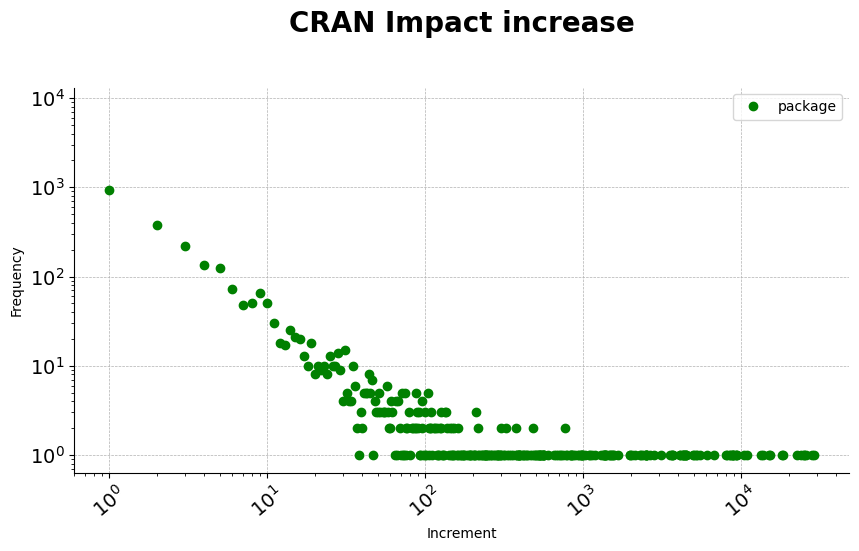
\includegraphics[width=1\textwidth]{img/cran/impact_increase_dist.png}
        \caption{Incremento de \textit{Impact}}
        \label{fig:Incremento de Impact}
    \end{center}
\end{figure}

Si lo representamos graficamente se obtiene una tendencia similar a las distribuciones anteriores. \ref{fig:Incremento de Impact}

\subsection{Alcance (\textit{Reach})}

El alcance (\textit{Reach}) de un paquete p, equivale al número de sucesores transitivos
de p más 1 y mide el número de paquetes potencialmente afectados
por un defecto en p.

A la vista de las siguientes tablas podemos observar que  paquetes
son los que tienenen un mayor reach. \ref{tab:Top 10 paquetes con mayor Reach}

\begin{table}[h!]
    \begin{center}
        \begin{tabular}{|c|c|}
            \hline
            \textbf{libraries.io} & \textbf{scraped} \\
            \hline
            R, 14395              & R, 17223         \\
            methods, 10839        & methods, 15103   \\
            utils, 10516          & utils, 15037     \\
            stats, 9850           & stats, 14360     \\
            graphics, 7938        & graphics, 12809  \\
            grDevices, 7382       & grDevices, 12763 \\
            Rcpp, 7380            & grid, 9241       \\
            lattice, 6296         & rlang, 8993      \\
            tools, 6127           & lattice, 8945    \\
            grid, 5971            & magrittr, 8916   \\
            \hline
        \end{tabular}
        \caption{Top 10 paquetes con mayor \textit{Reach}}
        \label{tab:Top 10 paquetes con mayor Reach}
    \end{center}
\end{table}

Si comparamos los resultados para ambos conjuntos de datos nos damos cuenta de que
los representantes de este top en su gran medida coinciden, esto es explicable ya que
el \textit{Reach} de un paquete depende de los paquetes que lo usan, y estos paquetes
en R suelen ser los más populares. \ref{fig:Top reach libraries.io} \ref{fig:Top reach scraped}


\begin{figure}[h!]
    \begin{center}
        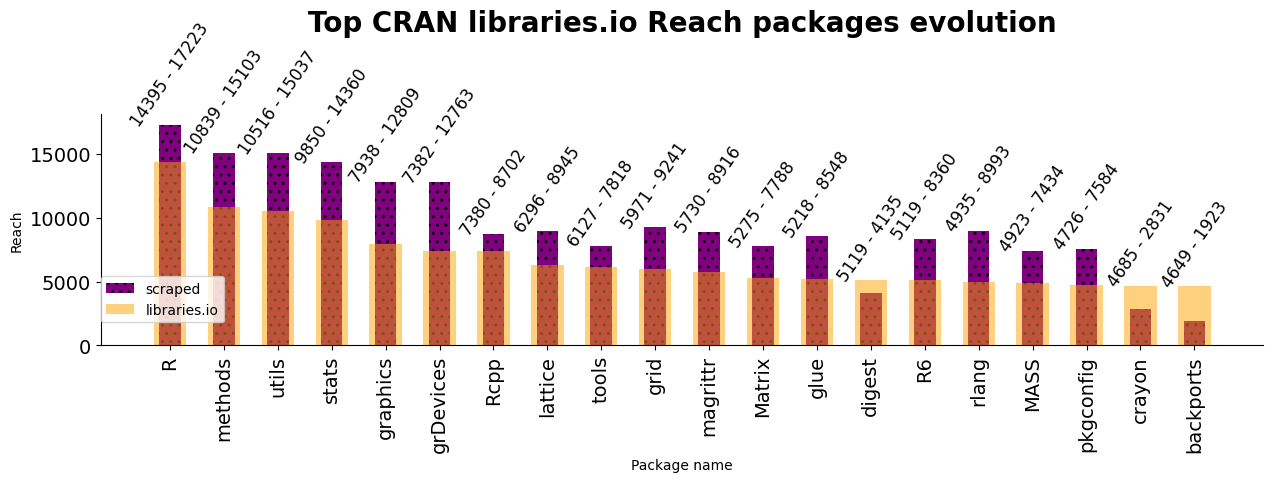
\includegraphics[width=1\textwidth]{img/cran/reach_top.png}
        \caption{Top paquetes con mayor \textit{Reach} en libraries.io}
        \label{fig:Top reach libraries.io}
    \end{center}
\end{figure}

\begin{figure}[h!]
    \begin{center}
        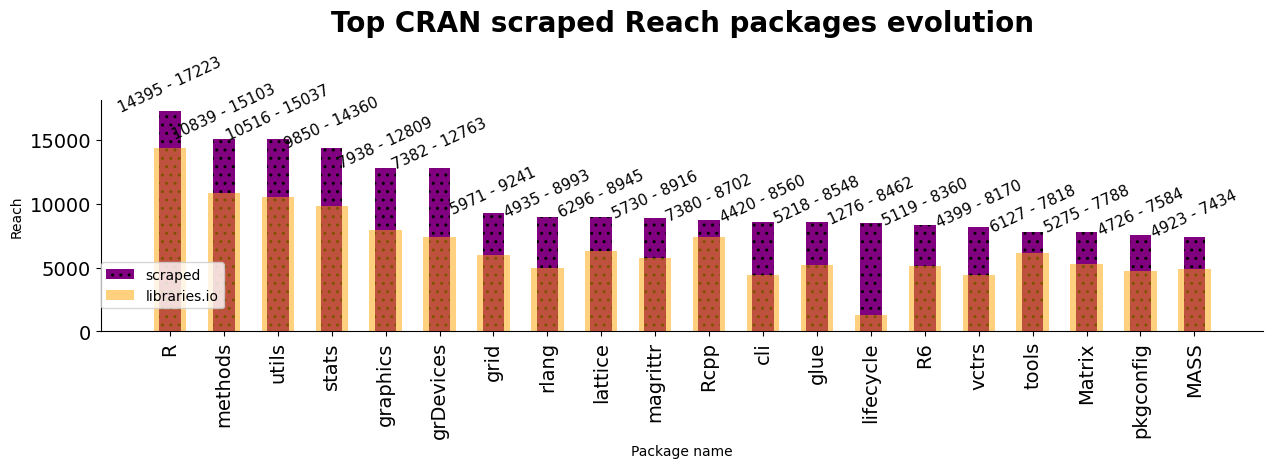
\includegraphics[width=1\textwidth]{img/cran/reach_top2.png}
        \caption{Incremento de \textit{Reach}}
        \label{fig:Top reach scraped}
    \end{center}
\end{figure}

Si observamos los paquetes con mayor incremento en \textit{Reach} \ref{tab:Top 10 paquetes con mayor incremento en Reach}
podemos ver que la mayoria estan presentes en el top, esta tabla nos da una idea de durante este periodo
de tiempo que paquetes han ganado mas dependientes.

\begin{table}[h!]
    \begin{center}
        \begin{tabular}{|c|c|c|c|}
            \hline
            \textbf{Paquete} & \textbf{libraries.io} & \textbf{scraped} & \textbf{increment} \\
            \hline
            lifecycle        & 1276                  & 8462             & 7186               \\
            grDevices        & 7382                  & 12763            & 5381               \\
            farver           & 48                    & 5020             & 4972               \\
            graphics         & 7938                  & 12809            & 4871               \\
            isoband          & 5                     & 4726             & 4721               \\
            utils            & 10516                 & 15037            & 4521               \\
            stats            & 9850                  & 14360            & 4510               \\
            splines          & 2016                  & 6466             & 4450               \\
            generics         & 457                   & 4895             & 4438               \\
            methods          & 10839                 & 15103            & 4264               \\
            \hline
        \end{tabular}
        \caption{Top 10 paquetes con mayor incremento en \textit{Reach}}
        \label{tab:Top 10 paquetes con mayor incremento en Reach}
    \end{center}
\end{table}

Es curioso ver que el paquete \textit{isoband} haya incrementado tanto su \textit{Reach}.
Este paquete es una implementación de la generación de bandas de confianza para curvas y mapas de contorno.
Resulta que este paquete fue protagonista de un incidente en el pasado:

El paquete \textit{isoband} estuvo en riesgo de ser archivado en \textit{CRAN}. La razón por la que este incidente causó
revuelo es que isoband es una dependencia de \textit{ggplot2} y cuando un paquete es eliminado de \textit{CRAN}, todos los
demás paquetes que dependen de él también son eliminados. Si isoband hubiera caído, \textit{ggplot2} estaría en
riesgo. Y esto habría desencadenado la eliminación de aún más paquetes. En total, la eliminación de
isoband habría llevado a la eliminación de 4747 paquetes\cite{r-bloggers_isoband_incident}.
Afortunadamente los desarrolladores de isoband pudieron solucionar el problema y el paquete no fue eliminado.
\cite{isoband_issue}.

Luego este incremento en el \textit{Reach} puede ser debido a que los desarrolladores de paquetes que dependen de isoband
se estan reenganchando al proyecto y actualizando sus paquetes para que sigan funcionando correctamente depues del incidente.



Por ultimo mostramos la distribucion de incremento de \textit{Reach} \ref{fig:Incremento de Reach}.

\begin{figure}[h!]
    \begin{center}
        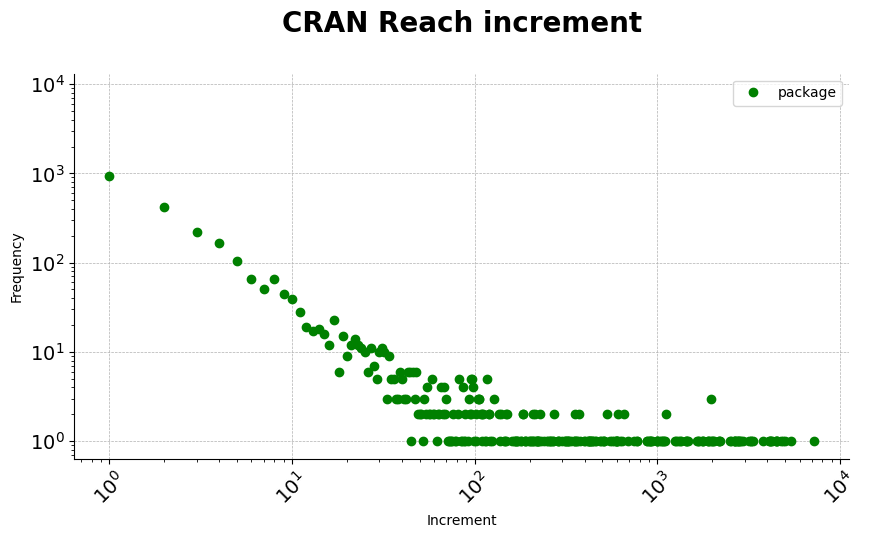
\includegraphics[width=0.8\textwidth]{img/cran/reach_increment.png}
        \caption{Incremento de \textit{Reach}}
        \label{fig:Incremento de Reach}
    \end{center}
\end{figure}


\newpage


\section{La red de dependencias de Bioconductor}

El repositorio \textit{Bioconductor} para R es una plataforma científica de código abierto que ofrece
herramientas y paquetes especializados para el análisis y la interpretación de datos genómicos.
Surgió en 2001 para abordar desafíos específicos de la biología computacional y la genómica.
\textit{Bioconductor} es reconocido por su calidad, diversidad y enfoque colaborativo. Proporciona
herramientas estadísticas y bioinformáticas para el análisis de expresión génica, variantes genéticas y más.
Su importancia radica en su contribución al avance de la investigación genómica y promoción de la
reproducibilidad y transparencia científica en el campo de la genómica y la biología computacional.

El análisis de \textit{Bioconductor} es necesario como complemento al análisis de CRAN debido a que se
enfoca específicamente en el análisis de un subconjunto del ecosistema R. Mientras que CRAN es el
repositorio principal de paquetes para el lenguaje de programación R, \textit{Bioconductor} se centra
en ofrecer herramientas especializadas para el análisis de datos genómicos y biológicos.

Además, es importante destacar que, en el contexto de \textit{Bioconductor}, se ha enfrentado el
desafío de la falta de datos de referencia en \textit{libraries.io}, un repositorio de información
sobre paquetes de software. Esto ha llevado a la necesidad de abrir nuevos caminos y proporcionar
un conjunto de datos que no existía previamente. Al hacerlo, se está facilitando el análisis y el
estudio de los paquetes de \textit{Bioconductor}, y se está contribuyendo a la disponibilidad de
datos valiosos para la comunidad.

\subsection{El tamaño}

La red de \textit{Bioconductor} es una red relativamente pequeña\ref{tab:Medidas de la red de dependencias de Bioconductor}
en comparacion con los valores de las otras redes que hemos analizado.
Los valores de las métricas indican una red de dependencias de \textit{Bioconductor} de tamaño bajo,
con alta conectividad entre los nodos.

\begin{table}[h!]
    \begin{center}
        \begin{tabular}{|l|c|}
            \hline
            \textbf{Medida}                & \textbf{Valor} \\
            \hline
            Number of nodes                & 3509           \\
            Number of edges                & 28320          \\
            Average degree                 & 16.14          \\
            Average clustering coefficient & 0.077          \\
            \hline
        \end{tabular}
        \caption{Medidas de la red de dependencias de Bioconductor}
        \label{tab:Medidas de la red de dependencias de Bioconductor}
    \end{center}
\end{table}

El coeficiente de agrupamiento promedio de aproximadamente 0.0776 sugiere que la red tiene un nivel moderado de agrupamiento.
Esto implica que algunos nodos están conectados en grupos o comunidades, pero no existe una fuerte tendencia hacia la formación
de comunidades densamente interconectadas en toda la red. Esto puede indicar que existen diferentes grupos temáticos o
funcionales dentro de la red de dependencias de \textit{Bioconductor}, pero también existen conexiones entre estos grupos.
Este coeficiente de agrupamiento es mucho menor que el de \textit{CRAN}, que era de 0.15.

Respecto al grado medio podemos decir que es un poco mayor que el de \textit{CRAN},
para el que teniamos un valor de 12.13.

\subsection{El grado}

A la vista de la distribución de \emph{grado} \ref{fig:bioconductor_degree_dist}, se puede observar una distribución
de \emph{ley de potencia}, lo cual es común en las \emph{redes de dependencias}.
En la gráfica, se puede apreciar que a partir de un \emph{grado} de 50, el
número de \emph{nodos} comienza a reducirse de manera exponencial, quedando
solo unos pocos representantes. Como era de esperar, se observan \emph{hubs}
o \emph{nodos de alto grado}, con valores cercanos a 2000. Esta presencia
de \emph{hubs} indica la existencia de elementos altamente conectados que
desempeñan un papel crucial en la estructura de la red de dependencias.

\begin{figure}[h!]
    \begin{center}
        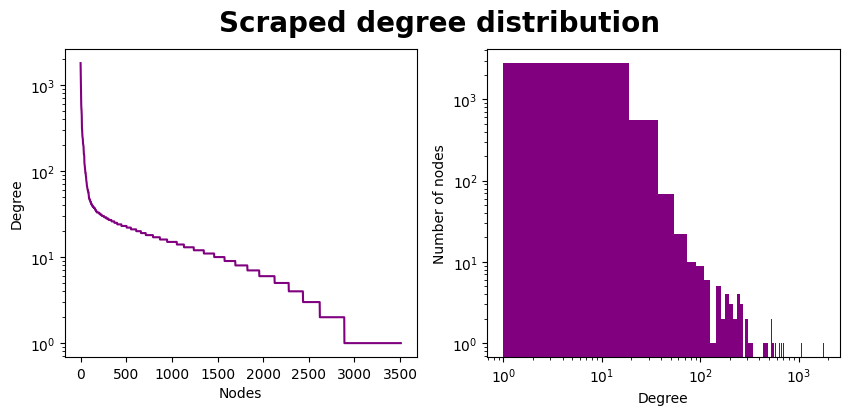
\includegraphics[width=1\textwidth]{img/bioconductor/degree_dist.png}
        \caption{Distribucion de grado de la red de dependencias de Bioconductor}
        \label{fig:bioconductor_degree_dist}
        \caption{Distribucion de grado de la red de dependencias de Bioconductor}
    \end{center}
\end{figure}

\subsubsection{El grado de salida \textit{Out degree}}

La distribución del \emph{grado de salida} en la red analizada presenta similitudes con
la distribución de la red de CRAN. En este caso, el \emph{grado de salida máximo} es
notablemente inferior debido al menor tamaño de la red, pero la tendencia general es
similar. Se puede apreciar que a partir de un \emph{grado de salida} de 10, la frecuencia
de individuos en la red se reduce significativamente. La mayoría de los nodos tienen un
\emph{grado de salida} inferior a 10, siendo estos el grupo más numeroso en la red.\ref{fig:bioconductor_out_degree_dist}

\begin{figure}[h!]
    \begin{center}
        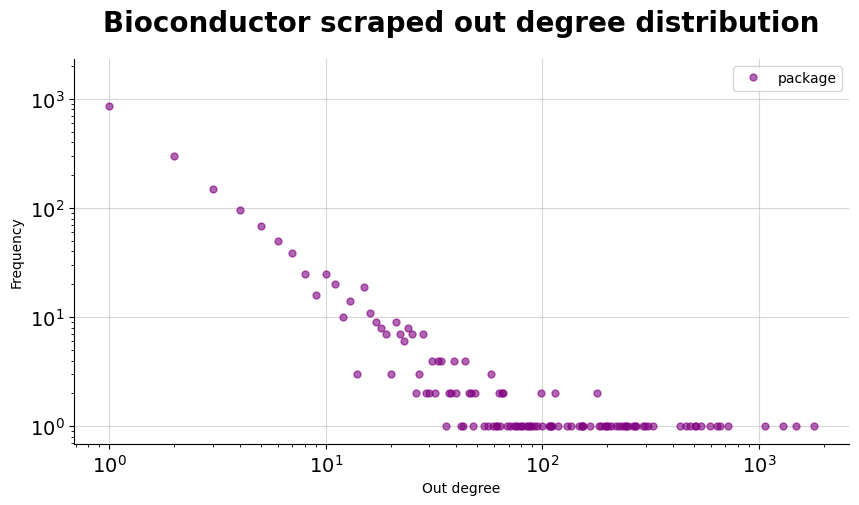
\includegraphics[width=0.8\textwidth]{img/bioconductor/out_degree_dist.png}
        \caption{Distribucion de grado de salida de la red de dependencias de Bioconductor}
        \label{fig:bioconductor_out_degree_dist}
    \end{center}
\end{figure}

En cuanto a los paquetes que representan el \emph{mayor grado de salida}\ref{fig:bioconductor_out_degree} 
en la red analizada, se observa que la mayoría de ellos también aparecen en el \emph{top} de la red de CRAN.
Este hallazgo es coherente, dado que, como se mencionó anteriormente, Bioconductor es un
subconjunto de los paquetes de R, y es esperable que estos paquetes tengan una importancia
similar en ambos repositorios.
Además, se observa que en este \emph{top} se encuentran los paquetes más importantes y exclusivos
de Bioconductor, como BiocGenerics o Biobase, entre otros. Esto nos indica que la red de Bioconductor
está especializada en el ámbito de la bioinformática, ya que estos paquetes desempeñan un papel crucial
en el análisis y procesamiento de datos biológicos. Su presencia en el \emph{top} indica la importancia
de la especialización de Bioconductor en este campo.

\begin{figure}[h!]
    \begin{center}
        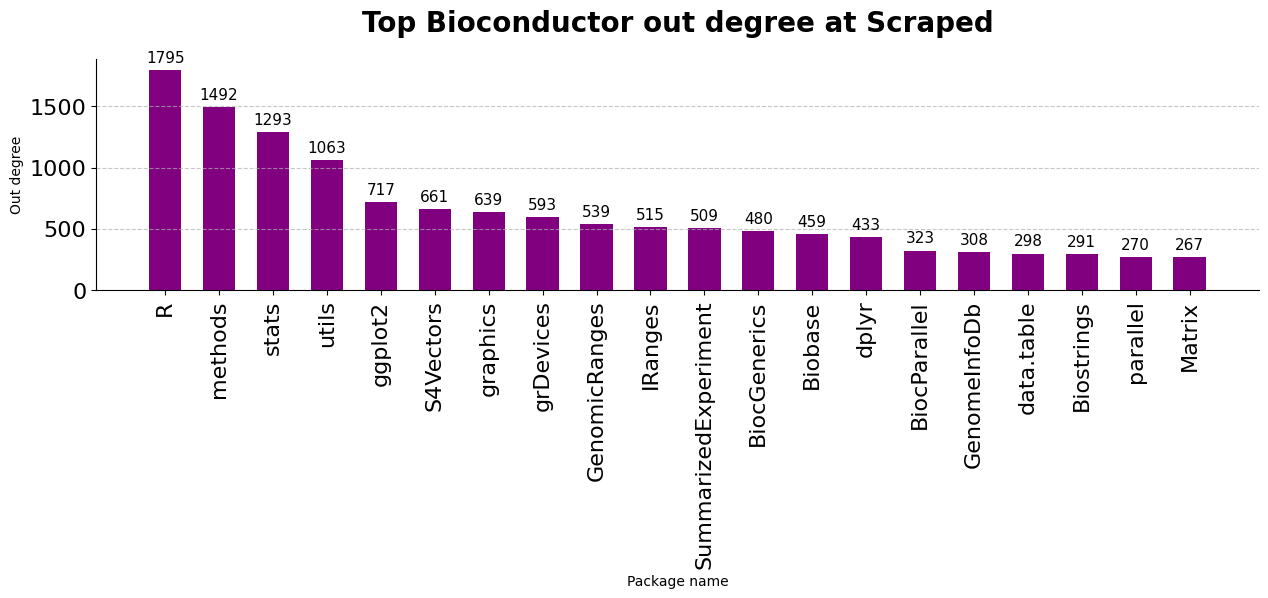
\includegraphics[width=1\textwidth]{img/bioconductor/top_out_degree.png}
        \caption{Top 10 de los paquetes con mayor grado de salida en la red de dependencias de Bioconductor}
        \label{fig:bioconductor_out_degree}
    \end{center}
\end{figure}


\subsubsection{El grado de entrada \textit{In degree}}

La distribución de \emph{in degree}\ref{fig:bioconductor_in_degree_dist} en la red de Bioconductor muestra algunas diferencias con respecto 
a la red de CRAN. Se observa que hay un menor número de nodos en la red de Bioconductor en comparación 
con CRAN. Además, la frecuencia máxima de nodos con \emph{in degree} ya no se encuentra en los valores 
1 o 2, como ocurre en CRAN. En Bioconductor, se puede apreciar que hay más nodos con \emph{in degree} 
en el rango de 10 a 20 en comparación con aquellos con un valor de 1.

Otro aspecto a tener en cuenta es que el \emph{in degree} máximo en la red de Bioconductor tiene un 
valor de 85, mientras que en CRAN el valor máximo es de 50. Esto indica que en Bioconductor existen 
nodos con un mayor número de dependencias entrantes, lo que podría reflejar la complejidad y la 
interconexión de los paquetes en Bioconductor. Estas diferencias en la distribución de \emph{in degree} 
evidencian las particularidades y características propias de la red de Bioconductor en comparación con 
la red de CRAN.

\begin{figure}[h!]
    \begin{center}
        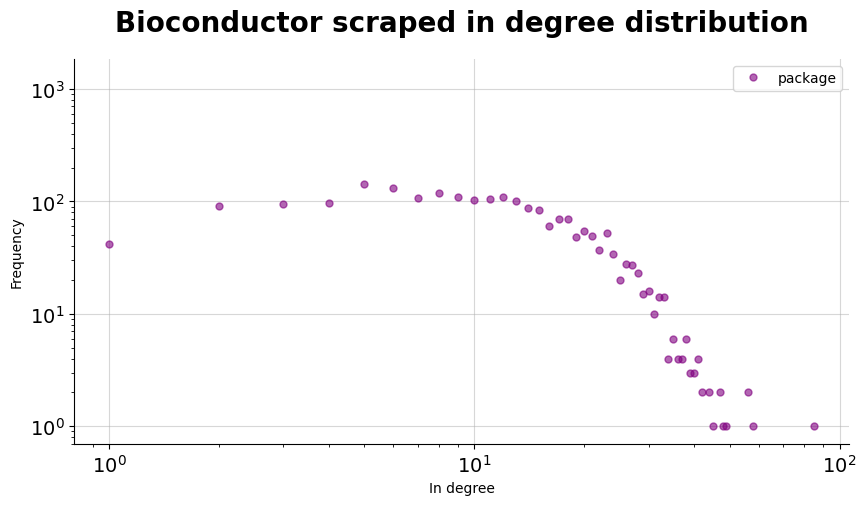
\includegraphics[width=0.8\textwidth]{img/bioconductor/in_degree_dist.png}
        \caption{Distribucion de grado de entrada de la red de dependencias de Bioconductor}
        \label{fig:bioconductor_in_degree_dist}
    \end{center}
\end{figure}

Los paquetes que se encuentran en el \emph{top} de \emph{grado de entrada} \ref{fig:bioconductor_in_degree} son aquellos que presentan 
un mayor número de dependencias en la red, sin tener en cuenta la transitividad de las conexiones. 
Esto implica que estos paquetes son altamente dependientes de otros paquetes en la red de Bioconductor en el primer nivel de 
profundidad del arbol de dependencias, lo que sugiere su importancia y relevancia en el ecosistema de Bioconductor. 

\begin{figure}[h!]
    \begin{center}
        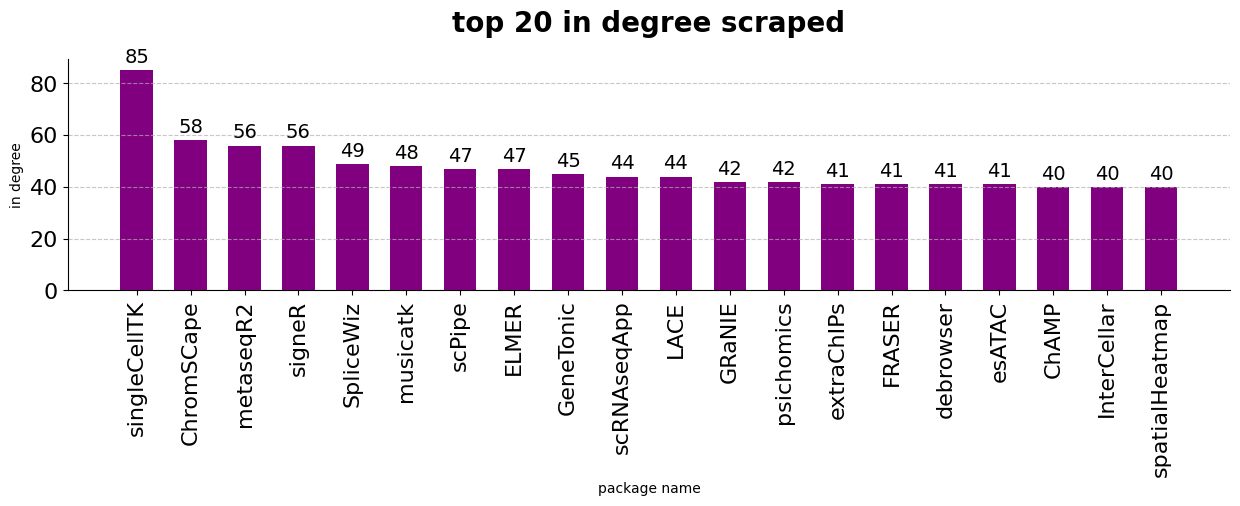
\includegraphics[width=1\textwidth]{img/bioconductor/top_in_degree.png}
        \caption{Top 10 de los paquetes con mayor grado de entrada en la red de dependencias de Bioconductor}
        \label{fig:bioconductor_in_degree}
    \end{center}
\end{figure}

\subsection{El PageRank}

La distribución de \textit{PageRank} \ref{fig:bioconductor_pagerank_dist} en la red de \textit{Bioconductor} no revela patrones claros 
y sencillos de analizar. Observando el gráfico, podemos determinar que la frecuencia máxima de nodos 
con el mismo valor de \textit{PageRank} se sitúa aproximadamente entre \textit{0.0002} y \textit{0.0005}. 
El rango normal de valores se encuentra entre \textit{0.0002} y \textit{0.002}, aunque en algunos casos 
particulares se alcanzan valores de \textit{0.003} o \textit{0.004}. Estos valores representan la importancia 
relativa de los nodos en la red, teniendo en cuenta tanto las conexiones directas como las conexiones 
indirectas a través de otros nodos en la red. Sin embargo, debido a la complejidad y tamaño de la red 
de \textit{Bioconductor}, es necesario realizar un análisis más detallado y específico para comprender 
plenamente la distribución y significado de los valores de \textit{PageRank} en esta red.

\begin{figure}[h!]
    \begin{center}
        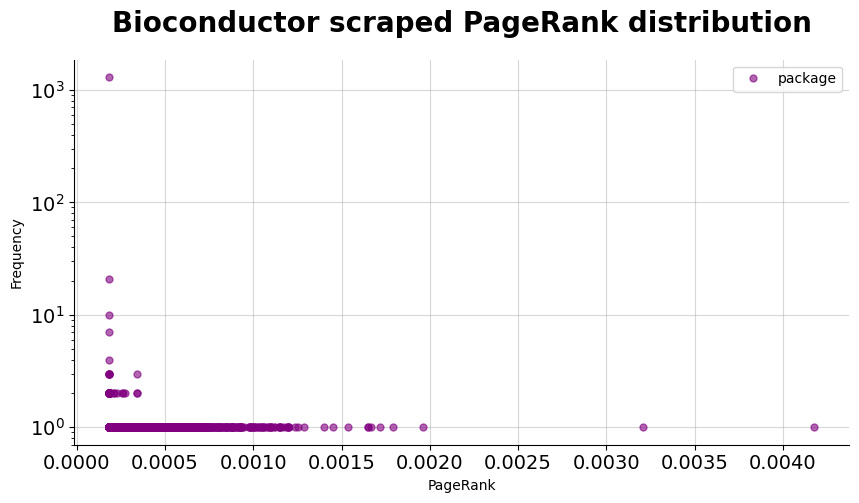
\includegraphics[width=1\textwidth]{img/bioconductor/pagerank_dist.png}
        \caption{Distribucion de PageRank de la red de dependencias de Bioconductor}
        \label{fig:bioconductor_pagerank_dist}
    \end{center}
\end{figure}


Respecto al top de dependencias con mayor \textit{PageRank} \ref{fig:bioconductor_top_pagerank_dependencies}, 
estos paquetes representan una vulnerabilidad significativa debido a su alto \textit{in degree} y la interconexión entre ellos. Desde el punto de vista 
del autor, sería recomendable evitar depender de alguno de estos paquetes, ya que se encuentran en un entorno 
donde la probabilidad de vulnerabilidad es mayor. La dependencia de estos paquetes puede aumentar la propagación 
de posibles problemas o errores a lo largo de la red de \textit{Bioconductor}. Por lo tanto, es esencial 
considerar alternativas y evaluar cuidadosamente las dependencias al desarrollar o utilizar aplicaciones 
basadas en esta red.

\begin{figure}[h!]
    \begin{center}
        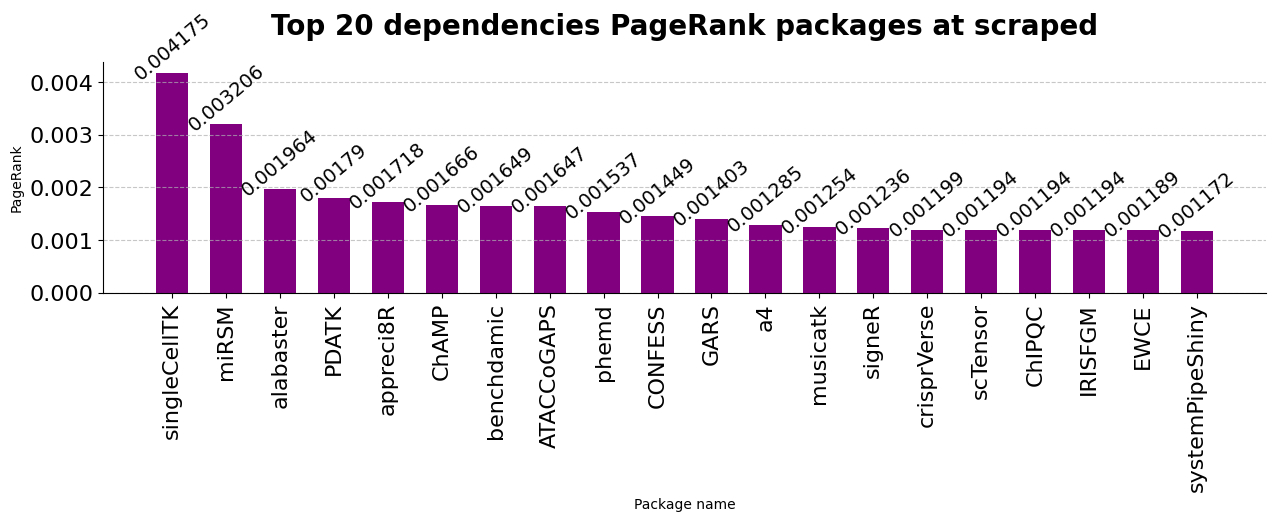
\includegraphics[width=1\textwidth]{img/bioconductor/top_pagerrank_dependencies.png}
        \caption{Top dependencias con mayor PageRank en la red de dependencias de Bioconductor}
        \label{fig:bioconductor_top_pagerank_dependencies}
    \end{center}
\end{figure}

Realizando una inversionde la red de dependencias de Bioconductor, se obtiene la red de paquetes, desde este punto de vista 
el \textit{PageRank} ahora esta ponderando la importancia de los paquetes en la red, es decir, aquellos paquetes que son dependencias
de otros paquetes importantes, son considerados como los mas importantes en la red. En la figura \ref{fig:bioconductor_top_pagerank_packages}
se muestran los paquetes con mayor \textit{PageRank} bajo este punto de vista de Bioconductor.

\begin{figure}[h!]
    \begin{center}
        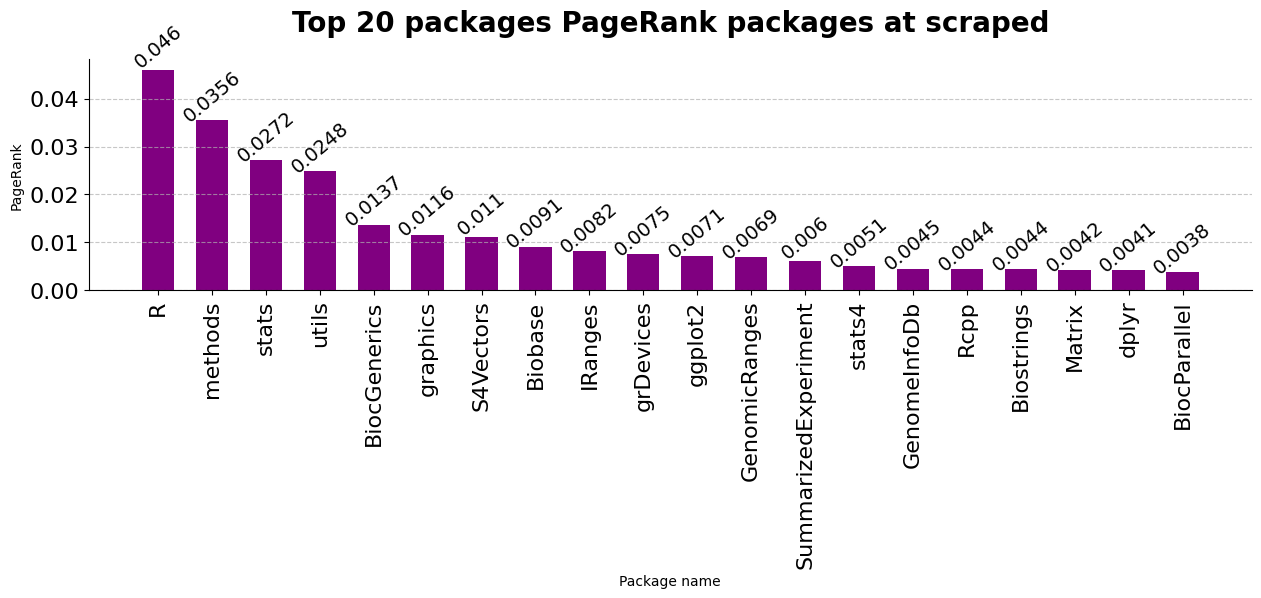
\includegraphics[width=1\textwidth]{img/bioconductor/top_pagerrank_packages.png}
        \caption{Top paquetes con mayor PageRank en la red de dependencias de Bioconductor}
        \label{fig:bioconductor_top_pagerank_packages}
    \end{center}
\end{figure}








\newpage

\section{La red de dependencias de PyPI}

En el ámbito del lenguaje de programación \textit{Python}, nos enfocamos en el análisis de \textit{PyPI}
(\textit{Python Package Index}). \textit{PyPI} es un repositorio ampliamente adoptado en la comunidad de
\textit{Python} debido a su facilidad de uso, su naturaleza de código abierto y su extensa colección de
paquetes.\footnote{Es importante mencionar que existen otros repositorios interesantes como \textit{Conda}.}

La facilidad de uso de \textit{PyPI} se deriva de su diseño intuitivo y las funcionalidades que ofrece
para la gestión de paquetes en \textit{Python}. Los desarrolladores pueden acceder a \textit{PyPI} como
una fuente centralizada para descubrir, descargar e instalar una amplia variedad de paquetes y bibliotecas
desarrollados por la comunidad.

En el análisis comparativo entre los datos proporcionados por \textit{libraries.io} y los recolectados en
este trabajo, se ha revelado una sorprendente tendencia en el número de paquetes presentes en \textit{PyPI}.
Se ha observado un aumento significativo en la cantidad de paquetes disponibles en \textit{PyPI} en
comparación con datos anteriores (en concreto un 474 \% ).

Este hallazgo sugiere un crecimiento notable en el ecosistema de paquetes de \textit{Python} y evidencia
el interés y participación de la comunidad en \textit{PyPI}. Este aumento en el número de paquetes puede
ser atribuido a diversos factores, como la creciente popularidad de \textit{Python} como lenguaje de
programación, el aumento en la adopción de \textit{Python} en diferentes campos de aplicación y el
creciente número de contribuyentes que comparten sus proyectos y soluciones a través de \textit{PyPI}.


\begin{figure}[h!]
    \begin{center}
        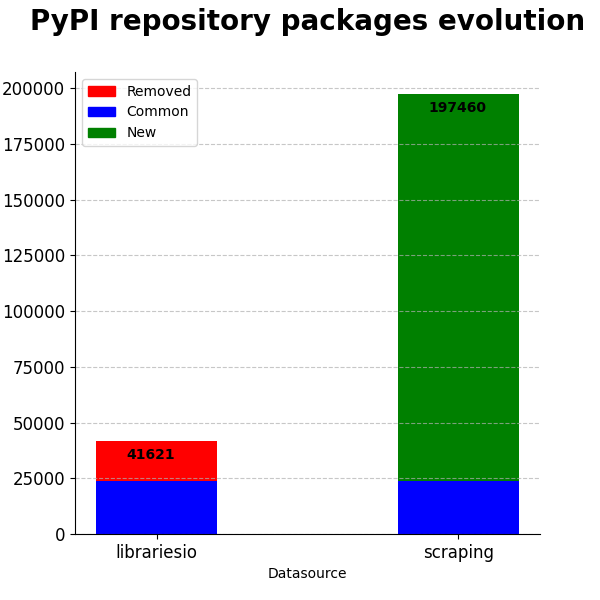
\includegraphics[width=0.6\textwidth]{img/pypi/bar_common_packages.png}
        \caption{Comparacion de la cantidad de paquetes en PyPI entre los datos de libraries.io y los recolectados en este trabajo.}
        \label{fig:pipy_common_packages_bar}
    \end{center}
\end{figure}

\begin{figure}[h!]
    \begin{center}
        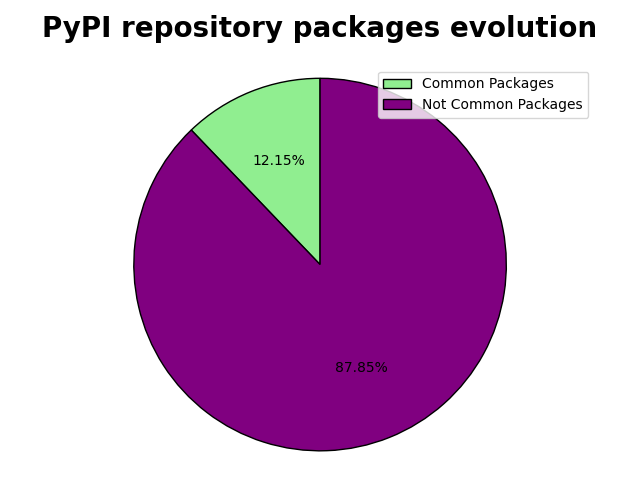
\includegraphics[width=0.6\textwidth]{img/pypi/circ_common_packages.png}
        \caption{Paquetes comunes y no comunes actualmente.}
        \label{fig:pipy_common_packages_circle}
    \end{center}
\end{figure}

El análisis de los datos revela que aproximadamente el \textit{57 \%} de los paquetes que estaban
presentes en el conjunto de datos antiguo de PyPI se han mantenido en el nuevo conjunto de datos
\footnote{Este porcentaje se basa en datos obtenidos experimentalmente.}. Este porcentaje
relativamente elevado indica que la red de paquetes en PyPI ha logrado mantener una cantidad considerable
de paquetes de manera estable a lo largo del tiempo \ref{tab:pypi_common_packages}.

\begin{table}[h!]
    \begin{center}
        \begin{tabular}{|l|r|}
            \hline
            \textbf{Descripción}                               & \textbf{Cantidad} \\
            \hline
            Paquetes en libraries.io                           & 41,621            \\
            Paquetes en scraped                                & 197,460           \\
            Paquetes comunes                                   & 24,001            \\
            Paquetes de libraries.io no disponibles en scraped & 17,620            \\
            Paquetes en scraped que no estan en libraries.io   & 173,459           \\
            \hline
        \end{tabular}
    \end{center}
    \label{tab:pypi_common_packages}
    \caption{Comparación de paquetes en PyPI entre los datos de libraries.io y los recolectados en este trabajo.}
\end{table}

Es importante destacar que este conjunto de paquetes que se ha mantenido representa aproximadamente
el \textit{12.15\%} del total de paquetes disponibles en PyPI en la actualidad. Esta proporción nos
proporciona una idea de la estabilidad relativa de la red, ya que una parte significativa de los
paquetes ha logrado mantener su presencia en PyPI a pesar de los posibles cambios y
actualizaciones\footnote{Los datos se refieren al momento de la última actualización y pueden estar
    sujetos a cambios futuros.}.

\begin{figure}[h!]
    \begin{center}
        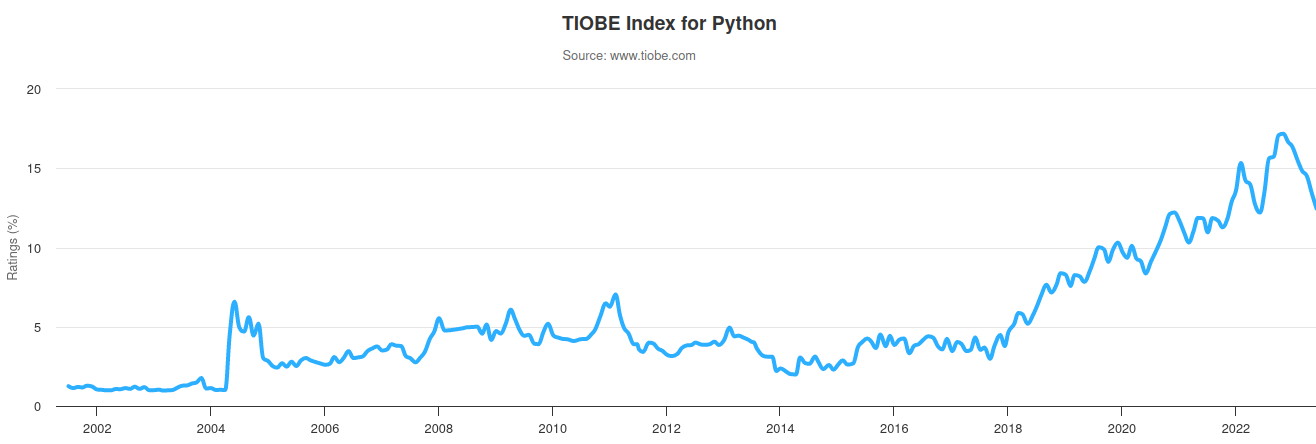
\includegraphics[width=1\textwidth]{img/pypi/pypi_popularity.png}
        \caption{Popularidad de Python a lo largo del tiempo.}
        \label{fig:pypi_popularity}
    \end{center}
\end{figure}


Esta tendencia en la popularidad de Python se ve reflejada en las estadísticas realizadas por la
empresa TIOBE \ref{fig:pypi_popularity}\footnote{\url{https://www.tiobe.com/tiobe-index/python/}}.


\subsubsection{Grado de la red}

Al examinar la distribución de grado en ambos conjuntos de datos, se observa que sigue una distribución
de ley de potencias\footnote{La distribución de ley de potencias es una característica común en las redes
    de dependencias.}.

Al analizar el gráfico, se evidencia que el grado máximo alcanzado por un paquete ha
experimentado un incremento significativo. Tomando como punto de referencia el número de nodos con grado
\textit{1000}, se puede apreciar una diferencia sustancial entre la red de \textit{libraries.io} y los
nuevos datos recolectados. Mientras que en \textit{libraries.io} se registran menos de \textit{10} paquetes
con dicho grado, en los nuevos datos se han identificado aproximadamente \textit{40} individuos
\footnote{Estos datos se basan en el análisis realizado en una fecha específica y pueden estar sujetos
    a cambios en el tiempo.}.

\begin{figure}[h!]
    \begin{center}
        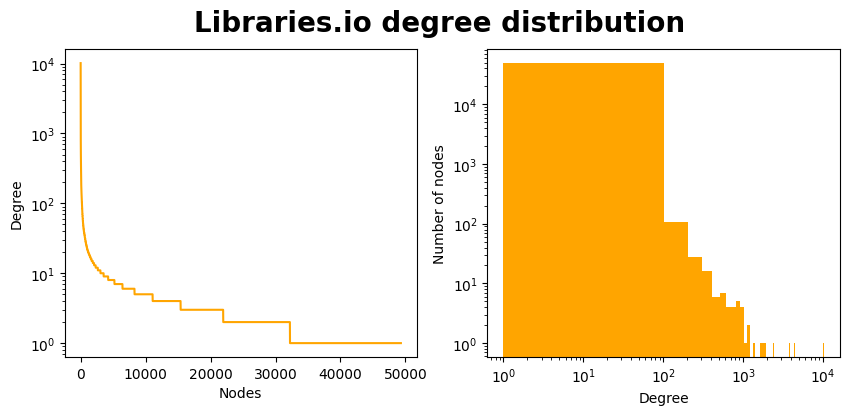
\includegraphics[width=0.8\textwidth]{img/pypi/librariesio_degree_distribution.png}
        \caption{Distribucion de grado de PyPI para libraries.io.}
        \label{fig:pypi_librariesio_degree_distribution}
    \end{center}
\end{figure}

\begin{figure}[h!]
    \begin{center}
        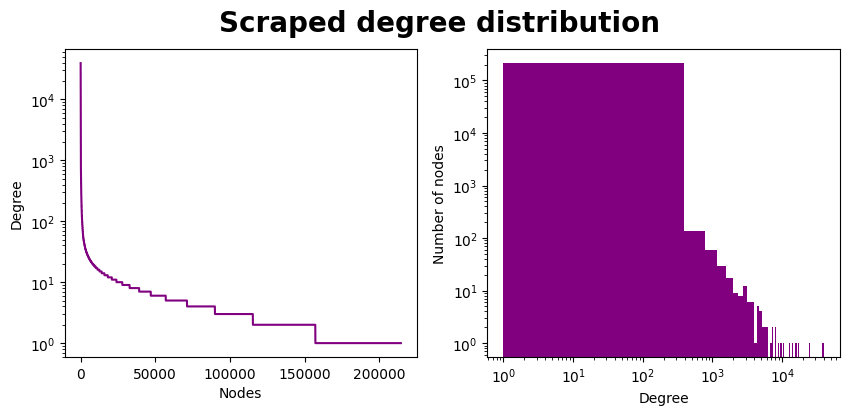
\includegraphics[width=0.8\textwidth]{img/pypi/scraped_degree_distribution.png}
        \caption{Distribucion de grado de PyPI para los datos recolectados.}
        \label{fig:pypi_scraped_degree_distribution}
    \end{center}
\end{figure}

Además, al calcular el grado promedio de los grafos correspondientes a \textit{libraries.io} y el nuevo
conjunto, se obtiene un valor de \textit{2.73} y \textit{4.35}, respectivamente. Estos valores indican
que, en promedio, cada paquete en la red de \textit{libraries.io} está conectado a alrededor de
\textit{2.73} otros paquetes, mientras que en los nuevos datos, cada paquete está conectado a
aproximadamente \textit{4.35} otros paquetes\footnote{Estos cálculos se realizaron utilizando una
    metodología específica y pueden variar dependiendo de la definición de conexión utilizada.}.

Estas estadísticas revelan cambios importantes en la estructura de la red de dependencias de paquetes.
El incremento en el grado máximo y el aumento en el grado promedio indican una mayor interconectividad
y complejidad en la red, lo cual puede ser atribuido al crecimiento y la evolución del ecosistema de
paquetes en Python.

Es importante destacar que la distribución de ley de potencias y la presencia de paquetes con grados
altos en la red tienen implicaciones significativas en términos de la propagación de dependencias y la
influencia de ciertos paquetes en la comunidad\footnote{Estas implicaciones pueden afectar la
    estabilidad, la modularidad y la confiabilidad del ecosistema de paquetes en Python.}.

\textbf{Grado de salida (\textit{out degree})}

El \textit{out degree} es una métrica que nos proporciona información
sobre el número de dependientes de un paquete dado. En el contexto de \textit{libraries.io},
analizando los datos, podemos identificar los paquetes que tienen más dependencias, es decir,
los que están en el \textit{Top} de las dependencias más utilizadas.


Los resultados obtenidos revelan una tendencia general en la cual las dependencias más populares han
experimentado un aumento en su popularidad, siendo ahora requeridas por un mayor número de paquetes
en la red de dependencias. En particular, se observa un incremento significativo en la popularidad
de las bibliotecas \textit{requests}, \textit{numpy}, \textit{pandas} y \textit{pytest} en comparación
con otros paquetes presentes en este ranking.

Estos hallazgos indican que estas bibliotecas han adquirido una mayor relevancia y utilidad en el
desarrollo de proyectos y aplicaciones en el entorno de Python.

\begin{figure}[h!]
    \begin{center}
        \includegraphics[width=1\textwidth]{img/pypi/libio_t20_outd_comparison.png}
        \caption{Top de paquetes con mayor grado de salida en PyPI para libraries.io }
        \label{fig:pypi_libio_outd_comparison}
    \end{center}
\end{figure}

\begin{figure}[h!]
    \begin{center}
        \includegraphics[width=1\textwidth]{img/pypi/libio_scraped_t20_comparation.png}
        \caption{Top de paquetes con mayor grado de salida en PyPI para scraped.}
        \label{fig:pypi_scraped_outd_comparison}
    \end{center}
\end{figure}

En este análisis de ranking, se observa que ciertos paquetes se han mantenido con respecto al ranking
anterior, lo cual indica su relevancia a lo largo del tiempo. Estos
paquetes incluyen \textit{PyYAML}, \textit{click}, \textit{numpy}, \textit{pandas}, \textit{pytest},
\textit{pyyaml}, \textit{requests}, \textit{setuptools} y \textit{six}. Su presencia continua en el
ranking sugiere que son dependencias fundamentales y ampliamente utilizadas en proyectos y aplicaciones
de Python\footnote{La relevancia y utilidad de estos paquetes se basa en la percepción de la comunidad
    de desarrolladores de Python y puede variar dependiendo del contexto y los requisitos del proyecto}.

Por otro lado, se identifican paquetes que han ascendido en el ranking en comparación con la clasificación
anterior. Estos paquetes incluyen \textit{black}, \textit{coverage}, \textit{flake8}, \textit{matplotlib},
\textit{odoo}, \textit{python}, \textit{scikit}, \textit{scipy}, \textit{sphinx}, \textit{tqdm} y
\textit{typing}. Su ascenso en el ranking puede ser atribuido a su creciente popularidad y utilidad en el
desarrollo de proyectos de Python, ya que son bibliotecas ampliamente conocidas y utilizadas por la
comunidad de desarrolladores\footnote{El ascenso en el ranking puede deberse a mejoras en funcionalidad,
    adopción en proyectos populares u otros factores que influyen en su popularidad}.

Por último, se muestra la distribución de \textit{out degree} para ambos conjuntos de datos \ref{fig:pypi_libio_outd_dist} \ref{fig:pypi_scraped_outd_dist}

\begin{figure}[h!]
    \begin{center}
        \includegraphics[width=0.8\textwidth]{img/pypi/outd_libio_dist.png}
        \caption{Distribución de \textit{Out degree} para libraries.io}
        \label{fig:pypi_libio_outd_dist}
    \end{center}
\end{figure}

\begin{figure}[h!]
    \begin{center}
        \includegraphics[width=0.8\textwidth]{img/pypi/outd_scraped_dist.png}
        \caption{Distribución de \textit{Out degree} para scraped}
        \label{fig:pypi_scraped_outd_dist}
    \end{center}
\end{figure}

Al analizar los gráficos de las distribuciones de \textit{out degree}, se observa una tendencia similar
en ambos conjuntos. Se evidencia un incremento general en el número total de paquetes, lo que indica un
crecimiento continuo en el ecosistema de paquetes.

Se ha observado un aumento en el número de paquetes con un grado de salida bajo, lo que indica que estos
paquetes tienen menos dependencias externas. Este fenómeno puede deberse a la introducción de paquetes
más autónomos y autosuficientes en el ecosistema de Python, lo que reduce la necesidad de depender de
otros paquetes para su funcionamiento.

Por otro lado, se ha identificado un incremento \ref{fig:dependents_increase} en el grado de salida de los paquetes más populares.
Esto indica que estos paquetes están siendo cada vez más utilizados como dependencias por otros paquetes
en la comunidad de Python. Este aumento en el grado de salida de los paquetes populares puede ser atribuido
a su funcionalidad ampliamente reconocida y popularidad.

\begin{figure}[h!]
    \begin{center}
        \includegraphics[width=0.8\textwidth]{img/pypi/dependents_increase.png}
        \caption{Incremento del \textit{Out degree} en PyPI}
        \label{fig:dependents_increase}
    \end{center}
\end{figure}


\textbf{Grado de entrada (\textit{In degree})}

Esta métrica nos da una idea del número de dependencias que tiene un paquete dado.
Analizados los datos de libraries.io y representados sobre un grafico obtenemos los siguientes resultados: \ref{fig:pypi_libio_ind_comparison}

\begin{figure}[h!]
    \begin{center}
        \includegraphics[width=1\textwidth]{img/pypi/libio_t20_ind_comparison.png}
        \caption{Top paquetes con mayor \textit{In degree} en libraries.io}
        \label{fig:pypi_libio_ind_comparison}
    \end{center}
\end{figure}

Se observa una tendencia decreciente en el número de dependencias entre los paquetes con mayor In degree
dentro del conjunto de bibliotecas de \textit{libraries.io}, lo cual sugiere una inclinación natural de los
paquetes hacia una disminución de las dependencias requeridas. Además, se aprecia que una proporción significativa
de estos paquetes, caracterizados por una elevada cantidad de dependencias, ha experimentado una desaparición,
representando aproximadamente un 25 \% de las instancias evaluadas. Por consiguiente, se puede inferir que,
en general, la presencia de un alto número de dependencias no suele correlacionarse con la estabilidad de
los paquetes en el repositorio.

\begin{figure}[h!]
    \begin{center}
        \includegraphics[width=1\textwidth]{img/pypi/scraped_t20_ind_comparison.png}
        \caption{Top paquetes con mayor \textit{In degree} en scraped}
        \label{fig:pypi_scraped_ind_comparison}
    \end{center}
\end{figure}

Si realizamos este mismo análisis con el top 20 de los paquetes con más \textit{In degree} en la actualidad \ref{fig:pypi_scraped_ind_comparison}, podemos llegar a
conclusiones similares. Se observa una tendencia decreciente en el número de dependencias de los paquetes
más influyentes, lo cual sugiere una reducción en la cantidad de paquetes que dependen directamente de ellos.
Esto puede indicar cambios en las estrategias de desarrollo, la aparición de alternativas o la evolución de la
comunidad de desarrolladores.

Estos hallazgos resaltan la importancia de considerar tanto el In degree como el grado de salida de
los paquetes al analizar la estabilidad y la evolución de la red de dependencias en el ecosistema de Python.

Como se puede apreciar, el \textit{95 \%} de los paquetes pertenecientes a este conjunto presentan una ausencia
de dependencias.
Si profundizamos en el tema, podemos apreciar que estos paquetes son de reciente aparición. La falta de
dependencias en los paquetes puede ser resultado de su diseño modular, el uso de
bibliotecas internas o la falta de necesidad de dependencias externas.

Cabe destacar un caso particular, el paquete denominado \textit{apache-airflow}
\footnote{\url{https://pypi.org/project/apache-airflow/}}, el cual ha experimentado un considerable aumento
en el número de dependencias, pasando de 41 a 185. La explicación que se atribuye a este fenómeno es la
incorporación de nuevas funcionalidades, dado que se trata de un paquete con cierta popularidad. No obstante,
desde la perspectiva del autor de este Trabajo Final de Grado, se recomienda a los desarrolladores reducir
al máximo este número de dependencias para mejorar su estabilidad\footnote{El aumento en el número de dependencias
    puede aumentar la complejidad y la posibilidad de conflictos en el entorno de desarrollo. Se sugiere evaluar
    cuidadosamente las dependencias necesarias y buscar alternativas más ligeras o mejor optimizadas si es posible}.

\begin{figure}[h!]
    \begin{center}
        \includegraphics[width=0.8\textwidth]{img/pypi/ind_libio_d.png}
        \caption{Distribucion del \textit{In degree} en libraries.io}
        \label{fig: Distribucion del In degree en libraries.io}
    \end{center}
\end{figure}

\begin{figure}[h!]
    \begin{center}
        \includegraphics[width=0.8\textwidth]{img/pypi/ind_scraped_dist.png}
        \caption{Distribucion del \textit{In degree} en scraped}
        \label{fig: Distribucion del In degree en scraped}
    \end{center}
\end{figure}

En el análisis de la distribución de In degree \ref{fig: Distribucion del In degree en libraries.io},
se ha observado una alta frecuencia de nodos con un bajo grado,
lo que indica la presencia de numerosos paquetes que no son utilizados como dependencias. Además, se ha identificado
una clara tendencia descendente en la frecuencia a medida que aumenta el \textit{In degree}.
Esto claramente representa una \textit{distribucion Power Law} \cite{enwiki:1160892030}.

La disminución en la frecuencia se vuelve significativa a medida que se alcanza un \textit{In degree} del orden
de $10^2$, donde la frecuencia se reduce a un único nodo por caso. Esto implica que existe una disminución drástica
en la cantidad de paquetes con un \textit{In degree} alto, lo cual sugiere que son menos comunes aquellos paquetes
que son ampliamente utilizados como dependencias por otros.

Si observamos la evolución \ref{fig: Distribucion del In degree en scraped}, se observa una tendencia similar en ambos casos, aunque en el estado actual se evidencia
un aumento en el número de nodos. La forma de la distribución se mantiene similar, pero se aprecia un considerable
incremento en el \textit{In degree}. Si consideramos la conclusión anteriormente obtenida, podemos constatar que
también se cumple en este caso, dado que el incremento en la frecuencia implica una disminución en el grado de
entrada.

\subsubsection{Pagerank}

La métrica de \textit{PageRank}\footnote{PageRank es un algoritmo utilizado para establecer un ranking de importancia en la web.}
nos permite establecer un ranking de importancia respecto a los paquetes. A la vista de la distribución obtenida de la red
de \textit{libraries.io}, una conclusión que se puede extraer es que la mayoría de las dependencias no son consideradas
importantes, ya que pertenecen al primer grupo, con una frecuencia considerablemente alta pero una baja relevancia en
términos de \textit{PageRank}. Sin embargo, existe un grupo más reducido pero significativo que presenta una importancia
media, pero son relevantes a nivel de que tienen múltiples enlaces provenientes de diferentes paquetes. Estas dependencias
comunes desempeñan un papel crítico en la interconexión de los diferentes componentes de la red. Además, se destaca
la presencia de un conjunto selecto de dependencias con un alto \textit{PageRank}, lo que indica su gran popularidad
y relevancia en la red de paquetes. En este grupo, las dependencias son enlazadas por muchas otras dependencias,
pero no tienen dependencias propias.

En concreto, estas son las dependencias más importantes a tener en cuenta debido a que suelen ser común su
aparición \ref{fig:Top 20 pagerank en libraries.io}.

\begin{figure}[h!]
    \begin{center}
        \includegraphics[width=1\textwidth]{img/pypi/libio_t20_pr_comparison.png}
        \caption{Top 20 \textit{PageRank} en libraries.io}
        \label{fig:Top 20 pagerank en libraries.io}
    \end{center}
\end{figure}


En términos de vulnerabilidad, los paquetes más críticos son aquellos que, si experimentan problemas o inestabilidad,
pueden tener un impacto significativo en toda la red de dependencias. Una dependencia crítica con múltiples enlaces
entrantes puede generar la propagación de errores o vulnerabilidades a través de los paquetes que dependen de
ella\footnote{Una dependencia crítica es aquella que, al presentar problemas, puede afectar negativamente a
    otros paquetes que dependen de ella, causando errores o vulnerabilidades en cadena.}.

Si visualizamos el número de dependencias transitivas \ref{fig:Dependencias transitivas del top 20 pagerank en libraries.io}
de estos paquetes, podemos obtener conclusiones más precisas.
Existe un grupo de paquetes con un menor número de dependencias transitivas, lo que los hace menos vulnerables en
comparación con el resto. Además, tener un alto \textit{PageRank} en estos paquetes implica que son más confiables
en términos de dependencias\footnote{Un paquete con un alto \textit{PageRank} y un bajo número de dependencias
    transitivas es considerado confiable y menos propenso a problemas de vulnerabilidad, ya que su estructura de
    dependencias es más simple y controlada.}.

\begin{figure}[h!]
    \begin{center}
        \includegraphics[width=1\textwidth]{img/pypi/transitive libraries.png}
        \caption{Dependencias transitivas del top 20 \textit{PageRank} en libraries.io}
        \label{fig:Dependencias transitivas del top 20 pagerank en libraries.io}
    \end{center}
\end{figure}

También se observa que en este grupo de paquetes, las dependencias transitivas son en promedio
más bajas\footnote{El número de dependencias transitivas en este grupo de paquetes tiende a
    ser menor en comparación con otros grupos, lo que indica una estructura más ligera y menos
    compleja en términos de dependencias.}.

Al analizar los resultados, se puede ver que los paquetes presentes en este grupo han
experimentado una evolución considerable \ref{fig:Top PageRank en scraped}, con una reducción significativa en
su \textit{PageRank}\footnote{El \textit{PageRank} de estos paquetes ha disminuido
    en comparación con mediciones anteriores.}. Esto se explica por la desaparición de algunos
de estos paquetes, la aparición de otros nuevos que han reemplazado su importancia y
la evolución de los propios paquetes hacia una mayor estabilización, lo que ha disminuido
su vulnerabilidad.

\begin{figure}[h!]
    \begin{center}
        \includegraphics[width=1\textwidth]{img/pypi/t20_dep_pr_scraped.png}
        \caption{Top \textit{PageRank} en scraped}
        \label{fig:Top PageRank en scraped}
    \end{center}
\end{figure}

Al examinar el nuevo conjunto de datos, se puede observar una tendencia similar a la anterior.
El aumento en el número de paquetes se refleja en una alta frecuencia de paquetes con un bajo
PageRank. Además, se observa una disminución general del valor del \textit{PageRank} en la mayoría de
la red. Esta disminución del \textit{PageRank} puede interpretarse como una mejora en términos de
vulnerabilidad.

Una conclusión que se puede extraer es que el crecimiento en el número de paquetes ha llevado
a una mayor presencia de paquetes con un bajo PageRank. Esto sugiere que hay una mayor
proporción de paquetes menos importantes en la red.

En este top se pueden observar las conclusiones previamente mencionadas en relación a la red de
dependencias. La mayoría de los paquetes en este conjunto son nuevos, lo que ha llevado a una
disminución del \textit{PageRank} en comparación con el caso anterior. Sin embargo, es
interesante destacar que algunos paquetes, como \textit{c3tools} y
\textit{gftools},
se mantienen en el top, lo que sugiere que han resistido bien el paso del tiempo y podrían
considerarse estables en la red, a pesar de tener una mayor probabilidad de
vulnerabilidad.

Además, se puede observar que los tres paquetes principales en este conjunto tienen
un \textit{PageRank} considerablemente más alto que el resto. Esta diferencia en
el \textit{PageRank} podría indicar que estos paquetes son especialmente relevantes
en la red de dependencias\footnote{Los tres paquetes principales en este conjunto son
    altamente influyentes y desempeñan un papel crucial en la interconexión de otros paquetes
    en la red de dependencias.}.

\begin{figure}[h!]
    \begin{center}
        \includegraphics[width=1\textwidth]{img/pypi/t20_pkg_pr_scr.png}
        \caption{Top \textit{PageRank} paquetes en scraped}
        \label{fig:Top PageRank paquetes en scraped}
    \end{center}
\end{figure}

Si invertimos el grafo de nuestra red de dependencias \ref{fig:Top PageRank paquetes en scraped}, podemos estudiar el \textit{PageRank}
desde el punto de vista de la relevancia del paquete en la red. Un alto \textit{PageRank}
implica que el paquete tiene una cantidad significativa de enlaces entrantes desde otros paquetes
importantes. Esto sugiere que el paquete es visto como una fuente confiable de información o
recursos dentro de la red. En otras palabras, es más probable que los otros paquetes dependan
del paquete con un alto \textit{PageRank} para obtener información o llevar a cabo determinadas
tareas.

Un paquete con un alto \textit{PageRank} puede ser considerado crucial en términos de la funcionalidad
o el rendimiento de la red. Es probable que los otros paquetes dependan directa o indirectamente de
él para llevar a cabo sus propias funciones o tareas.

Como se puede ver en el top que mostramos a continuación, aparecen los paquetes más conocidos y
comúnmente usados de Python para los dos conjuntos de datos.

\subsubsection{Impacto (Impact)}

El impacto de un paquete se refiere al número de dependencias que se verían afectadas si
ocurriera un defecto en ese paquete. Esta métrica podría utilizarse para evaluar la criticidad
o importancia de un paquete en la red de dependencias y ayudar en la identificación de los
paquetes que tienen un mayor impacto en el sistema en caso de fallos.

\begin{table}[h!]
    \centering
    \caption{Comparación entre paquetes obtenidos de libraries.io y scraped para la metrica impact}
    \begin{tabular}{|c|c|c|}
        \hline
        \textbf{libraries.io} & \textbf{scraped}   \\
        \hline
        six, 36757            & numpy, 448177      \\
        certifi, 18739        & six, 424014        \\
        requests, 17740       & python, 422180     \\
        pyparsing, 14111      & importlib, 420861  \\
        packaging, 13433      & typing, 417287     \\
        appdirs, 12619        & colorama, 416663   \\
        setuptools, 11803     & matplotlib, 414520 \\
        python-dateutil, 9825 & chardet, 413067    \\
        numpy, 7396           & Cython, 412181     \\
        pytz, 6878            & click, 411954      \\
        \hline
    \end{tabular}
\end{table}


Resulta interesante apreciar que los paquetes del top siguen siendo prácticamente los mismos
pese al notable incremento del impacto y que además esta métrica se relaciona bastante con el
Pagerank a nivel de paquete.

\begin{figure}[h!]
    \begin{center}
        \includegraphics[width=1\textwidth]{img/pypi/librariesio_impact_distribution.png}
        \caption{Distribución del impacto en la red de libraries.io}
        \label{fig:Distribución del impacto en la red de libraries.io}
    \end{center}
\end{figure}

A la vista de la distribución del impacto en la red de libraries.io \ref{fig:Distribución del impacto en la red de libraries.io}, se observa un patrón que se
asemeja al comportamiento de la distribución del grado de salida (\textit{out degree}). Se puede notar
que existen numerosos paquetes con un impacto bajo, y la única explicación plausible es que estos paquetes
no son ampliamente utilizados como dependencias en otros paquetes.

Es común que la mayoría de los paquetes tengan un impacto relativamente bajo, en el rango de alrededor
de 10 paquetes. A medida que aumentamos el valor del impacto, la frecuencia de paquetes con un impacto
alto disminuye significativamente.

Este patrón sugiere que la mayoría de los paquetes en la red de libraries.io no tienen una influencia
crítica en las dependencias y, por lo tanto, su fallo o defecto tendría un impacto limitado en el
sistema en general. Sin embargo, se
identifican ciertos paquetes cuyo impacto es notablemente mayor, lo cual indica que son cruciales
y tienen una influencia significativa en las dependencias.

\begin{figure}[h!]
    \begin{center}
        \includegraphics[width=1\textwidth]{img/pypi/scraped_impact_distribution.png}
        \caption{Distribución del impacto en la red scraped}
        \label{fig:Distribución del impacto en la red scraped}
    \end{center}
\end{figure}

Al evaluar el estado actual de la red, se observan cambios significativos en la distribución del
impacto, que muestra similitudes con la distribución del grado de salida (\textit{out degree}),
aunque también presenta variaciones y la formación de grupos con tendencias similares.

En particular, se ha observado un considerable aumento en el impacto general de los paquetes en la
red. Ahora se identifica la presencia de un número considerable de paquetes con un impacto del orden
de 10², lo cual indica que su influencia en las dependencias ha aumentado
significativamente.

Además, se distingue un segundo grupo más reducido de paquetes con un impacto alto, en el orden de 10000.
Este grupo de paquetes merece especial atención debido a su impacto significativo
en la red de dependencias.

Asimismo, se ha identificado otro grupo no existente anteriormente que resulta notable debido a
su impacto elevado.


Al analizar el incremento del impacto en la red de dependencias, se observa una distinción entre
dos casos. Por un lado, hay paquetes que han experimentado una disminución en su nivel de impacto
o han mantenido un grado de \emph{vulnerabilidad} estable a lo largo del tiempo. Por otro lado,
existen paquetes que han experimentado un aumento significativo en su impacto.

Es notable que estos paquetes que han experimentado un aumento considerable en su impacto
están interrelacionados y forman parte de componentes altamente conectados dentro de la red.
Esta \emph{interconexión} entre los paquetes permite un aumento grupal del impacto, amplificando
así la magnitud de las consecuencias en caso de fallos o defectos.

\begin{table}[h!]
    \centering
    \caption{Comparación del incremento del impacto para de libraries.io, scraped}
    \begin{tabular}{|c|c|c|c|}
        \hline
        \textbf{Paquete} & \textbf{libraries.io} & \textbf{scraped} & \textbf{incremento} \\
        \hline
        numpy            & 7396                  & 448177           & 440781              \\
        importlib        & 24                    & 420861           & 420837              \\
        colorama         & 1795                  & 416663           & 414868              \\
        typing           & 2434                  & 417287           & 414853              \\
        matplotlib       & 748                   & 414520           & 413772              \\
        Cython           & 75                    & 412181           & 412106              \\
        chardet          & 1707                  & 413067           & 411360              \\
        BeautifulSoup4   & 75                    & 411391           & 411316              \\
        genshi           & 5                     & 411290           & 411285              \\
        cssselect        & 260                   & 411490           & 411230              \\
        \hline
    \end{tabular}
\end{table}


A la vista del top de incremento del impacto se aprecia similitud entre los paquetes seleccionados,
los cuales resultan muy familiares para los desarrolladores que usamos el lenguaje Python ya que
son paquetes muy usados en casi todo tipo de software.

Si analizamos el decremento se puede ver que no es tan acentuado como el incremento, no
podemos sacar muchas conclusiones de ello más que estos paquetes han disminuido el número de
dependencias transitivas que poseían, simplemente quedémonos con observar la tendencia y ver qué
paquetes han sido los más afectados. \ref{tab:Disminución del impacto en libraries.io y scraped}

\begin{table}[h!]
    \centering
    \label{tab:Disminución del impacto en libraries.io y scraped}
    \begin{tabular}{|c|c|c|c|}
        \hline
        \textbf{Paquete}              & \textbf{librariesio} & \textbf{scraped} & \textbf{incremento} \\
        \hline
        python-dateutil               & 9825                 & 0                & -9825               \\
        importlib-metadata            & 4677                 & 0                & -4677               \\
        backports.functools-lru-cache & 1944                 & 0                & -1944               \\
        async-timeout                 & 1828                 & 0                & -1828               \\
        asn1crypto                    & 2503                 & 817              & -1686               \\
        oslo.i18n                     & 1503                 & 0                & -1503               \\
        futures                       & 2277                 & 816              & -1461               \\
        oslo.utils                    & 1242                 & 0                & -1242               \\
        singledispatch                & 1213                 & 87               & -1126               \\
        pyasn1-modules                & 1101                 & 0                & -1101               \\
        \hline
    \end{tabular}
    \caption{Disminución del impacto en libraries.io y scraped}
\end{table}




\subsubsection{Reach}

La métrica llamada \emph{Reach} , que se refiere a la vulnerabilidad
frente a fallos en una red de paquetes, se utiliza para medir el alcance de los paquetes afectados
por un fallo aleatorio en la red. Se define como la media aritmética del alcance de los nodos
en la red.

La vulnerabilidad de la red se cuantifica al calcular el número esperado de paquetes comprometidos
por un fallo aleatorio, asumiendo que las probabilidades de fallo son independientes y siguen
una distribución uniforme.

A nivel de paquete se refiere al número de paquetes que se verían afectados por un fallo en un
paquete o alguna de sus dependencias transitivas, es decir el número de sucesores transitivos
de un paquete más 1.\footnote{El alcance a nivel de paquete se
    define como el número de paquetes que se verían afectados por un fallo en un paquete o alguna
    de sus dependencias transitivas.}.


\begin{figure}[h!]
    \begin{center}
        \includegraphics[width=1\textwidth]{img/pypi/top_librariesio_reach_evolution.png}
        \caption{Top Reach en libraries.io}
    \end{center}
\end{figure}


Bajo esta definición, al analizar el top 20 de paquetes con el mayor \textit{Reach} en una red compuesta por aproximadamente 40000 nodos, resulta llamativo observar que algunos paquetes
presentan un \textit{Reach} tan elevado. Además, es importante destacar que estos paquetes se
encuentran entre los más populares y utilizados en Python, lo cual justifica el valor alcanzado.
Sin embargo, desde el punto de vista de la vulnerabilidad de la red, resulta preocupante, ya que
un fallo en alguno de estos paquetes representaría un peligro significativo.

En relación a estos paquetes, en el estado actual de la red, resulta sorprendente el incremento
que han experimentado en su alcance. Este incremento puede ser explicado por el crecimiento en el
número de nodos de la red. Estos valores destacados para los paquetes en cuestión nos proporcionan
una idea clara de la vulnerabilidad que introduce su presencia en la red. Si consideramos que
\textit{PyPI} actualmente cuenta con aproximadamente \textit{200000} paquetes, un fallo en alguno de estos paquetes
que se encuentran en el \textit{top} del ranking tendría un impacto \textit{considerable} en la integridad de la red.


\begin{figure}[h!]
    \begin{center}
        \includegraphics[width=1\textwidth]{img/pypi/top_scraped_reach_evolution.png}
        \caption{Top Reach en scraped}
    \end{center}
\end{figure}


Si comparamos las distribuciones de \textit{reach} para los dos conjuntos de datos, podemos ver que tienen una
tendencia similar a la distribución de \textit{grado de salida}.

\begin{figure}[h!]
    \begin{center}
        \includegraphics[width=0.8\textwidth]{img/pypi/librariesio_reach_distribution.png}
        \caption{Distribución del Reach en libraries.io}
    \end{center}
\end{figure}

\begin{figure}[h!]
    \begin{center}
        \includegraphics[width=0.8\textwidth]{img/pypi/scraped_reach_distribution.png}
        \caption{Distribución del Reach en scraped}
    \end{center}
\end{figure}

El nuevo conjunto de datos muestra la existencia de tres grupos distintos. El primer grupo presenta
un valor de \textit{Reach} bajo, lo que indica que no hay un nivel significativo de vulnerabilidad. En el
segundo grupo, el valor de \textit{Reach} se sitúa en el orden de \textit{10000}, lo cual representa un riesgo mayor.
Aunque el número de paquetes pertenecientes a este grupo no es excesivamente alto, es importante
tenerlo en cuenta debido a su nivel de vulnerabilidad. Por último, el tercer grupo se caracteriza
por tener un valor de \textit{Reach} muy alto.

Según mi interpretación, estos dos grupos de alto Reach representan nodos pertenecientes a componentes
fuertemente conexos y son en los que habría que poner el foco para proteger la estabilidad de la red.

\begin{figure}[h!]
    \begin{center}
        \includegraphics[width=0.8\textwidth]{img/pypi/reach_increment.png}
        \caption{Incremento del Reach}
    \end{center}
\end{figure}

En relación al incremento del Reach, se pueden identificar dos tendencias distintas. En la primera
tendencia, se observa que el Reach se mantiene relativamente estable, con fluctuaciones dentro de un
rango aproximado de ±15,000. Por otro lado, el segundo grupo exhibe un notable aumento en el valor
del Reach. Un fallo en un paquete perteneciente a este grupo podría generar graves problemas en la red.
Este incremento puede ser atribuido al crecimiento en el número de nodos de la red. Como resultado de
este crecimiento, han surgido dependencias transitivas que han contribuido significativamente a este
aumento considerable en el Reach.

\subsubsection{Componente fuertemente conexo}

En un \textit{componente fuertemente conexo}, todos los nodos están directa o indirectamente conectados
entre sí. No importa si los caminos son directos o implican múltiples pasos a través de otros nodos,
lo fundamental es que existe una ruta dirigida desde cualquier nodo al resto de los nodos del componente.

Bajo la red de libraries.io no se identifican componentes fuertemente conexos. Esto se debe principalmente
al tamaño de la red, que es relativamente pequeño. Sin embargo, en el nuevo conjunto de datos, se ve claramente
la existencia de componentes fuertemente conexos. \ref{table:scc}

\begin{table}
    \begin{tabular}{|c|c|c|c|c|c|c|c|}
        \hline
        \textbf{Size} & \textbf{Avg}    & \textbf{Density} & \textbf{Diameter} & \textbf{Clustering}  & \textbf{Transitive}   \\
                      & \textbf{degree} &                  &                   & \textbf{coefficient} & \textbf{dependencies} \\
        \hline
        283           & 8.890           & 0.015            & 14                & 0.196                & 206873                \\
        9             & 4.947           & 0.137            & 8                 & 0.358                & 23807                 \\
        8             & 3.000           & 0.214            & 6                 & 0.222                & 6288                  \\
        8             & 5.250           & 0.375            & 3                 & 0.383                & 6784                  \\
        8             & 4.750           & 0.339            & 5                 & 0.498                & 6752                  \\
        6             & 5.000           & 0.500            & 2                 & 0.776                & 4536                  \\
        6             & 4.666           & 0.466            & 3                 & 0.470                & 4452                  \\
        6             & 3.666           & 0.366            & 3                 & 0.448                & 4440                  \\
        5             & 2.800           & 0.350            & 4                 & 0.000                & 3770                  \\
        5             & 6.000           & 0.750            & 2                 & 0.777                & 3855                  \\
        5             & 3.200           & 0.400            & 4                 & 0.386                & 3765                  \\
        5             & 3.600           & 0.450            & 3                 & 0.421                & 3755                  \\
        4             & 3.000           & 0.500            & 3                 & 0.406                & 5276                  \\
        4             & 2.500           & 0.416            & 3                 & 0.000                & 3016                  \\
        4             & 3.000           & 0.500            & 3                 & 0.406                & 3220                  \\
        4             & 3.000           & 0.500            & 3                 & 0.700                & 2988                  \\
        4             & 3.000           & 0.500            & 3                 & 0.406                & 3048                  \\
        4             & 3.000           & 0.500            & 3                 & 0.406                & 3064                  \\
        4             & 4.500           & 0.750            & 2                 & 0.800                & 2948                  \\
        3             & 2.666           & 0.666            & 2                 & 0.000                & 3780                  \\
        \hline
    \end{tabular}
    \caption{Componentes fuertemente conexos}
    \label{table:scc}
\end{table}

A partir de estos datos, se pueden extraer varias conclusiones. Existen componentes fuertemente conexos de diversos
tamaños, desde pequeños hasta muy grandes. Algunos componentes tienen una alta importancia medida por el pagerank
del nodo principal. La densidad y el coeficiente de agrupamiento varían entre los componentes, lo que sugiere diferentes
patrones de conexiones. Además, el número de dependencias transitivas varía ampliamente en funcion del tamaño del componente.

\begin{figure}[h!]
    \begin{center}
        \includegraphics[width=1\textwidth]{img/pypi/scc1_dist.png}
        \caption{Distribucion de grado del mayor componente fuertemente conexo}
    \end{center}
\end{figure}

\begin{figure}[h!]
    \begin{center}
        \includegraphics[width=1.2\textwidth]{img/pypi/scc1.png}
        \caption{Mayor componente fuertemente conexo}
    \end{center}
\end{figure}


\capitulo{6}{Trabajos relacionados}

Los gestores de paquetes de software son herramientas esenciales que facilitan la reutilización y
la construcción eficiente de sistemas de software. Estos gestores permiten a los desarrolladores y
profesionales de la informática acceder a bibliotecas de código previamente desarrolladas, lo que
agiliza el proceso de desarrollo al evitar tener que crear funcionalidades desde cero.

Dado que el software se distribuye a través de estos gestores de paquetes, es crucial para los
investigadores y profesionales tener acceso a datos explícitos sobre las redes de dependencia
de software. Estas \textit{redes de dependencia} están compuestas por las relaciones entre los
diferentes \textit{paquetes de software} y pueden resultar opacas si no se cuenta con información precisa.

Para poder analizar y razonar sobre los ecosistemas y productos de software cada vez más
complejos, los investigadores y profesionales dependen de conjuntos de datos públicos disponibles.
Un ejemplo de ello es el conjunto de datos publicado en \textit{libraries.io}, sin embargo,
lamentablemente ha quedado desatendido y no se ha actualizado con regularidad.

Aquí es donde entra en juego el valor de este trabajo en particular, ya que proporciona un nuevo
conjunto de datos que se centra en los gestores de paquetes \textit{CRAN}, \textit{Bioconductor},
\textit{PyPI} y \textit{npm}. Estos conjuntos de datos actualizados ofrecen una perspectiva más
reciente y completa sobre la información disponible hasta la fecha. Esto es especialmente relevante
para los autores de trabajos relacionados que han utilizado el conjunto de datos de \textit{libraries.io}
en sus investigaciones, ya que ahora tienen la oportunidad de actualizar sus estudios utilizando
esta nueva información más actualizada. Con esto, se puede mejorar la calidad de la investigación
y garantizar que los resultados y conclusiones reflejen con precisión el estado actual de los
ecosistemas de software.

A continuación se presentan algunos de los trabajos relacionados que han utilizado el conjunto de
datos de \textit{libraries.io} en sus investigaciones.
\begin{itemize}
    \item \textbf{On the impact of security vulnerabilities in the npm and rubygems dependency networks} \cite{zerouali2022impact}:
          Este artículo estudia empíricamente las vulnerabilidades de seguridad que afectan a los paquetes npm y RubyGems.
          Analiza cómo y cuándo se descubren y solucionan estas vulnerabilidades y cómo cambia su prevalencia con el tiempo.
          También analiza cómo los paquetes vulnerables exponen a sus dependientes directos e indirectos a vulnerabilidades.
    \item \textbf{Dependency solving is still hard, but we are getting better at it} \cite{abate2020dependency}:
          Este artículo trata sobre la resolución de dependencias, que es un problema difícil (NP-completo) en todos los modelos
          de componentes no triviales debido a versiones mutuamente incompatibles de los mismos paquetes o conflictos de
          paquetes declarados explícitamente.
    \item \textbf{On the usage of JavaScript, Python and Ruby packages in Docker Hub images} \cite{zerouali2021usage}:
          Este artículo analiza empíricamente el uso de paquetes de terceros de JavaScript, Python y Ruby en imágenes de Docker Hub.
          Estudia cuán prevalentes, desactualizados y vulnerables son estos paquetes en imágenes de la comunidad que se basan en
          imágenes base de node, Python y Ruby.
    \item \textbf{Mining single statement bugs at massive scale} \cite{richter2022tssb}:
          Este artículo presenta un enfoque para extraer y analizar bugs de una sola declaración de código fuente de proyectos
          de software.
    \item \textbf{Technical lag of dependencies in major package managers} \cite{stringer2020technical}:
          Este artículo trata sobre el retraso técnico de las dependencias en los principales gestores de paquetes.
          Las bibliotecas de terceros utilizadas por un proyecto (dependencias) pueden quedar fácilmente desactualizadas con el
          tiempo, un fenómeno llamado retraso técnico.
    \item \textbf{Identifying critical projects via pagerank and truck factor} \cite{pfeiffer2021identifying}:
          Este artículo trata sobre la identificación de proyectos críticos a través de PageRank y el factor de eje (Truck Factor).
          Recientemente, el equipo de código abierto de Google presentó el puntaje de criticidad, una métrica para evaluar la
          “influencia e importancia” de un proyecto en un ecosistema a partir de señales específicas del proyecto, como el número
          de dependientes, la frecuencia de confirmación, etc.
    \item \textbf{Identifying versions of libraries used in stack overflow code snippets} \cite{zerouali2021identifying}:
          Este artículo trata sobre la identificación de versiones de bibliotecas utilizadas en fragmentos de código de Stack Overflow.
    \item \textbf{Intertwining Communities: Exploring Libraries that Cross Software Ecosystems} \cite{kannee2023intertwining}:
          Este artículo trata sobre la exploración de bibliotecas que cruzan ecosistemas de software.
\end{itemize}
\capitulo{7}{Conclusiones y Líneas de trabajo futuras}


\section{Conclusiones}

En esta conclusion se pretende dar una introducción al escaneo y análisis de repositorios software, destacando la dificultad asociada debido
a la \emph{elevada cantidad de datos}\footnote{La cantidad de datos almacenados en los repositorios software puede ser enormemente extensa,
    lo que implica desafíos en términos de procesamiento y almacenamiento.} y la necesidad de comprender la temática de los mismos. Se ha de tener en cuenta
también el \emph{tiempo de ejecución}\footnote{El tiempo requerido para realizar un escaneo y análisis exhaustivo de un repositorio puede
    ser considerable debido a la cantidad de operaciones y tareas involucradas.} y el \emph{gasto de recursos}\footnote{El análisis de grandes
    volúmenes de datos puede requerir altos consumos de memoria RAM y espacio en disco, lo que puede afectar el rendimiento general del sistema.}
asociados a esta tarea. La computacion en la nube es una solución a estos problemas, ya que permite el procesamiento de grandes volúmenes de
datos de forma distribuida, escalable y eficiente.

Respecto a la persistencia de los datos, la elección entre una base de datos y archivos CSV para almacenar los datos de las redes de dependencias 
de paquetes depende de varios factores. Si se requiere una estructura de datos más compleja, consultas sofisticadas y escalabilidad a largo plazo, 
una base de datos es la opción más adecuada. Sin embargo, si se trabaja con conjuntos de datos más pequeños, se valora la simplicidad y la portabilidad, 
y no se necesitan capacidades avanzadas de gestión de datos, los archivos CSV pueden ser una solución práctica y eficiente.
En nuestro caso, se ha optado por el uso de archivos CSV debido a la simplicidad de la estructura de datos y ser la estructura usada por OLIVIA para
almacenar los datos de las redes de dependencias de paquetes. No obstante, se ha de tener en cuenta que el uso de archivos CSV puede implicar
problemas, por lo que se recomienda el uso de una base de datos para el almacenamiento de los datos por las ventajas que ofrecen en términos de 
rendimiento y escalabilidad.
Sobre el almacenamiento en GitHub, se ve necesario \emph{particionar los datos} ya que existe una limitación en el tamaño máximo de archivo de 100 MB.

En cuanto a la extracción de datos, se ha de tener en cuenta que la extracción de datos de los repositorios software es una tarea compleja debido
a la gran cantidad de información que se puede extraer de los mismos. Por ello, se ha de tener en cuenta que la extracción de datos debe ser
\emph{flexible y extensible}, ya que se pretende que sea capaz de adaptarse a diferentes repositorios software y a diferentes tipos de análisis.

En cuanto al análisis de los datos, el análisis de los datos es una tarea compleja debido a la naturaleza amplia y compleja de la ciencia de redes. 
Requiere el uso de técnicas y herramientas especializadas, así como un profundo conocimiento y comprensión de los principios de la ciencia de redes. 
Sin embargo, este análisis puede brindar información valiosa sobre las interdependencias y la estructura de los paquetes mas importantes en los repositorios software,
proponemos una vision general de los paquetes mas importantes respecto a distinta metricas de centralidad y aportamos una vision de evolucion de los paquetes
al comparar los resultados de libraries.io con los obtenidos por en este trabajo.

Por último, se propone el diseño de una herramienta capaz de llevar a cabo la recoleccion de datos, gestionando
los posibles inconvenientes que puedan surgir durante el proceso. Se ha de tener en cuenta que el diseño de la herramienta debe ser extensible, 
ya que se pretende que sea capaz de adaptarse a diferentes repositorios software y a diferentes tipos de análisis y debido a su
naturaleza opensource y experimental, se ha realizado un esfuerzo adicional en la documentación del código y en el control de calidad del mismo.


\section{Líneas de trabajo futuras}

\subsection{Mejoras en la herramienta}

Con el objetivo de mejorar la herramienta desarrollada, se identifican diversas áreas de enfoque. 
En primer lugar, se propone realizar mejoras en el diseño y pulir detalles técnicos para optimizar su rendimiento y eficiencia. 
Esto implica revisar y refinar la arquitectura de la herramienta, identificar posibles cuellos de botella y aplicar técnicas de 
optimización que permitan un procesamiento más rápido y una mayor escalabilidad.

Adicionalmente, se propone añadir soporte para nuevos repositorios, con el fin de ampliar la compatibilidad de la herramienta y 
permitir su aplicación en una variedad de entornos y plataformas. Esto implica adaptar la herramienta para interactuar con 
diferentes sistemas de control de versiones y repositorios, asegurando la interoperabilidad y facilitando su adopción por 
parte de un mayor número de usuarios.

Por último, es necesario replantearse la persistencia de datos. Esto implica evaluar la forma en que se almacenan y gestionan 
los datos recolectados durante el análisis de los repositorios software. Se pueden considerar opciones como el uso de bases de 
datos para un almacenamiento más eficiente y la implementación de mecanismos de respaldo y recuperación de datos para garantizar
 su integridad y disponibilidad a largo plazo.

\subsection{Análisis de los datos}

Se propone realizar un análisis más exhaustivo a partir de los datos recolectados. Esto implica la aplicación de técnicas de análisis
de redes complejas para identificar patrones y tendencias en las redes de dependencias de paquetes. Ahí entra la comunidad científica, que puede
aportar una visión más amplia y profunda de los datos que aportamos en este trabajo, así como una mayor comprensión de los mismos. Esto permitirá 
obtener información con la que actualizar sus investigaciones continuar con el estudio de las redes de dependencias de paquetes.

\subsection{Herramienta de visualización}

Sería un punto interesante el desarrollo de una herramienta de visualización que permita representar gráficamente las redes de dependencias
de paquetes y el calculo de metricas asociadas. Esto implica el diseño e implementación de una interfaz gráfica de usuario que permita la 
interacción con la herramienta y la visualización de los resultados del análisis de los repositorios software. Esto permitirá a los usuarios
explorar y comprender mejor las redes de dependencias de paquetes, así como identificar patrones y tendencias en los datos.



\bibliographystyle{plain}
\bibliography{bibliografia}

\end{document}
